\documentclass[hidelinks, 4pt]{bookest}
\usepackage{bera}
\renewcommand*\familydefault{\sfdefault}

\let\orignewcommand\newcommand  % store the original \newcommand
\let\newcommand\providecommand  % make \newcommand behave like \providecommand
\RequirePackage{verse}
\let\newcommand\orignewcommand  % use the original `\newcommand` in future
\makeatletter
% Use the original definition from verse.sty
\renewcommand*{\theHpoemline}{\arabic{verse@envctr}.\arabic{poemline}}
\makeatother

%tamanho do documento
\geometry{paperwidth=16cm, paperheight=23cm}

%codificação
\usepackage{siunitx}
\usepackage[utf8]{inputenc}
\usepackage[T1]{fontenc}

%lingua
\usepackage[brazilian]{babel}

%hifen
\usepackage{hyphenat}

%urls
\usepackage{hyperref}

%cor,eumerar, tabela, legenda, verso, tamanho de tabela
\usepackage{color}
\usepackage[hang, splitrule]{footmisc}
\usepackage{enumerate}
\usepackage{booktabs}
\usepackage{wrapfig}
\usepackage[center, small]{titlesec}
\usepackage{caption}
\usepackage{multirow}
\usepackage{longtable}
\usepackage{graphicx}
\usepackage{adjustbox}
\usepackage{array} % for defining a new column type
\usepackage{doi}
\usepackage{pdfpages}
\usepackage{mathtools}
\usepackage{afterpage}
\usepackage[shortlabels]{enumitem}
\usepackage{layouts}
\usepackage{tocloft}
\renewcommand{\cftdot}{}
\setlength{\cftsecnumwidth}{0pt}
\setlength{\cftsubsecnumwidth}{46pt}

%fontes para imagens e tabelas
\captionsetup[figure]{font=scriptsize}
\captionsetup[table]{font=scriptsize}
\setlength{\captionmargin}{30pt}

%rodapé vazio
\makeatletter
\def\blfootnote{\xdef\@thefnmark{}\@footnotetext}
\makeatother

%cabeçalho
\usepackage{fancyhdr}
\fancyhead[LE,RO]{\scriptsize \slshape \rightmark}
\fancyhead[LO,RE]{}
\fancyfoot[C]{\thepage}
\pagestyle{fancy}
\renewcommand{\chaptermark}[1]{\markright{#1}{}}
\renewcommand{\sectionmark}[1]{\markright{#1}{}}

\newcommand\blankpage{%
    \null
    \thispagestyle{empty}%
    \addtocounter{page}{-1}%,
    \newpage}

\fancypagestyle{myplain}
{
  \fancyhf{}
  \renewcommand\headrulewidth{0pt}
  \renewcommand\footrulewidth{0pt}
  \fancyfoot[C]{\thepage}
}

\newcounter{nopage}
\newenvironment{nopage}
 {\clearpage\stepcounter{nopage}%
  \renewcommand{\thepage}{}%
  \thispagestyle{empty}}
 {\clearpage\addtocounter{page}{-1}}

\makeatletter
\def\cleardoublepage{\clearpage\if@twoside \ifodd\c@page\else
    \hbox{}\thispagestyle{myplain}\newpage\if@twocolumn\hbox{}\newpage\fi\fi\fi}
    \pagenumbering{arabic}
\makeatother

\begin{document}
%\includepdf{capa.pdf}
%\pagebreak
\begin{titlepage}
    \vspace*{\fill}
    \begin{center}
        {\Huge Debates sobre feminismo e Análise do Comportamento}
    \end{center}
    \vspace*{\fill}
    \pagestyle{empty}
    \afterpage{\null\newpage}
    \blankpage
\begin{center}
    \vfill
\end{center}
\begin{center}
{\Large Renata Pinheiro e Táhcita Medrado }\\[4cm]
{\Huge Debates sobre feminismo e Análise do Comportamento}\\[4cm]

{\Large Primeira Edição}\\[3cm]


{\large Fortaleza\\
Imagine Publicações}

2019
\pagebreak
\thispagestyle{empty}
\end{center}
\pagebreak

Copyright\textsuperscript{\textcircled{c}} 2019 da 1ª edição pela Imagine Publicações Ltda.\\

ISBN: 978-85-54337-00-1

Capa: -

Coordenação: Felipe Leite

Edição: Roberto Leite

Editor de Planejamento: Hernando Borges Neves Filho

Comitê Editorial: Hernando Borges Neves Filho, Felipe Leite e

Roberto Leite

Revisão: Letícia Mota

Projeto gráfico e editoração eletrônica: João Pedro Magalhães\\
\vfill
\begin{center}
%\includegraphics[width=0.9\textwidth]{catalografico.png} \\
\end{center}

2019

Todos os direitos em língua portuguesa reservados pela

IMAGINE PUBLICAÇÕES LDTA.

Rua Doutor Gilberto Studart, 55 - Sala 1502 - T1

CEP: 60192-105 - Cocó - Fortaleza - CE

Telefone: (85) 3246-1706

Email: editora@imaginetc.com.br\\

Impresso no Brasil pela Arte Visual Gráfica e Editora, Fortaleza-Ce
\thispagestyle{empty}
\end{titlepage}
\begin{nopage}
\chapter*{Debates sobre Feminismo e Análise do Comportamento}\sectionmark{Prefácio: Debates sobre Feminismo e Análise do Comportamento}
\begin{center}
    \textbf{\large Prefácio}
\end{center}

Quando pensamos a organização desse livro, na ocasião da 47ª Reunião Anual da Sociedade Brasileira de Psicologia (SBP), em outubro de 2017, não imaginávamos a proporção que ele tomaria. O objetivo era reunir um material voltado para a discussão da desigualdade de gênero na análise do comportamento, especialmente quando a ausência dessa discussão em muitos textos com os quais nos formamos analistas do comportamento mantinha isso invisível. Nesse caminho, descobrimos e redescobrimos muitos trabalhos e pesquisadoras e o resultado foi impressionante. Nós somos muitas! Foi inspirador ler os trabalhos e descobrir como a análise do comportamento pode contribuir para a área de estudos de gênero e, também, se beneficiar dela. Daí se formou o segundo objetivo deste livro: visibilizar essas pesquisadoras e essa produção. Para isso, no primeiro capítulo, as autoras Gabriela Jheniffer Teixeira da Silva e Ana Arantes expõem o processo de invisibilização da mulher na ciência, especificamente na Análise do Comportamento, e resgatam um pouco dessa história representada – ou não representada – na literatura da área.

No segundo capítulo, Táhcita Medrado Mizael escreve sobre algumas formas de articulação entre a análise do comportamento e o feminismo interseccional. No terceiro capítulo, Laís Nicolodi e Ana Arantes operacionalizam os conceitos de poder e patriarcado a partir do referencial analítico-comportamental. Em seguida, no quarto capítulo, Amanda Oliveira de Morais e Júlia Castro de Carvalho Freitas discorrem sobre cultura do estupro e os diferentes métodos de investigação deste fenômeno dentro e fora da psicologia e da análise do comportamento. 

No quinto capítulo, Madeleine Reinert Marcelino e Ana Arantes utilizam o conceito de atitudes implícitas e pesquisas sobre este tema para evidenciar como práticas machistas e opressoras podem ser fortalecidas na história de vida dos indivíduos. No sexto capítulo, Aline Guimarães Couto traz diferentes noções sobre o empoderamento da mulher e os discute sob um ponto de vista analítico-comportamental.

No sétimo capítulo, Júlia Cavalcanti Ferraz, Hellen Luane Silva Peixinho, Christian Vichi e Angelo A. S. Sampaio, utilizam os conceitos de metacontingência, macrocontingência e macrocomportamento para analisar a prática de assédio sexual verbal. No oitavo capítulo, Izadora Ribeiro Perkoski faz uma análise sobre os aspectos culturais e intervenções comportamentais que possibilitem o aumento da participação feminina na área da computação. 

No nono capítulo, Renata da Conceição da Silva Pinheiro e Cláudia Kami Bastos Oshiro apresentam e discutem algumas contingências que comumente aparecem nas demandas de clientes mulheres em processo psicoterápico e que possuem um claro viés de gênero. Seguindo na mesma linha clínica, no décimo capítulo, Analu Ianik Costa discute aspectos teóricos sobre relacionamentos abusivos e possibilidades de intervenção, aplicando-os em um estudo de caso.

Acreditamos que esse livro chega num momento muito oportuno, acadêmica e politicamente. O interesse crescente pela área, o desenvolvimento de estudos mais culturais e socioverbais e a expressão de políticas que se mostram contrárias a igualdade de gênero proposta pelo feminismo mostram como o conteúdo deste livro pode ser útil e se tornar uma ferramenta de estudo e de luta. Dessa forma, compartilhamos o conteúdo desse livro com vocês, esperando que eles as e os inspirem como inspiraram a nós. Convidamos vocês também a olharem, a seguir, as fotos e minicurrículos de todas as autoras que juntas construíram esse material conosco. Seguimos juntas.
\addtocontents{toc}{\cftpagenumbersoff{section}}
\addtocontents{toc}{\cftpagenumbersoff{subsection}}
\tableofcontents
\end{nopage}
\addtocounter{page}{-8}
\chapter*{Apresentação}
\section*{Por que Feminismo na Análise do Comportamento?}
\begin{flushright}
    \emph{Carolina Laurenti}
\end{flushright}

Ecos do ativismo do movimento feminista começaram a ressoar no contexto acadêmico na década de 1960, e foram ganhando mais projeção entre o fim dos anos 1970 e início da década de 1980, inclusive na psicologia. Desde então, as críticas feministas a determinadas formas de se produzir conhecimento científico têm desafiado a ciência de um modo geral, e a psicologia em particular, a se tornar uma prática cultural mais justa, igualitária e democrática, deixando de reproduzir, subscrever ou mesmo encorajar desigualdades entre gêneros verificadas em diferentes esferas da sociedade. 

A interlocução entre Análise do Comportamento e Feminismo no âmbito acadêmico foi principiada, sobretudo, pelos trabalhos de Maria del Rosario Ruiz (1950-2017), que explorou, do ponto de vista teórico-filosófico, algumas afinidades entre teses feministas e a filosofia do comportamentalismo radical. As produções dessa autora, entretanto, parecem não ter sido suficientes para inserir a Análise do Comportamento de modo mais expressivo nesse cenário, considerando, até o momento, a escassa produção que discute essa aliança na área \footnote{Ver Couto, A.,\& Dittrich, A. (2017). Feminismo e análise do comportamento: Caminhos para o diálogo. Revista: Perspectivas em Análise do Comportamento, 8(2), 147-158.}.

No Brasil, o diálogo entre Feminismo e Análise do Comportamento é recente e relativamente incipiente. A despeito do caráter embrionário desses estudos no país, tem acontecido uma série de iniciativas com o intuito de propiciar um contexto favorável à discussão de temas fomentados pelo Feminismo acadêmico. O livro “Debates sobre Feminismo e Análise do Comportamento” é uma expressão lídima desse esforço, e preenche uma lacuna importante no tocante à produção nacional acerca do Feminismo. Mas não se trata “apenas” de um livro sobre Feminismo. É um livro sobre a Análise do Comportamento – a sua história, teoria, ciência e profissão – discutida de uma perspectiva de gênero. Esse viés dá relevo a aspectos usualmente negligenciados na narrativa historiográfica dessa disciplina (e.g., as diferentes mulheres que participaram da institucionalização e consolidação dessa disciplina no Brasil), bem como permite perscrutar temas que pouco integram as agendas de pesquisa do campo (e.g., patriarcado, machismo, cultura do estupro, empoderamento feminino, práticas de gênero, assédio sexual, interseccionalidade, participação feminina na computação, psicoterapia feminista). É, antes de tudo, um livro sobre a práxis acadêmico-científica dos/as analistas do comportamento, o seu lugar social e suas implicações ético-políticas.

Um livro como este certamente enfrentará e, ao mesmo tempo, lançará muitos desafios para a Análise do Comportamento. Um deles é justamente discutir Feminismo. Isso porque existem conotações pejorativas do termo bastante difundidas no senso comum que podem tolher, logo de início, qualquer tentativa de debate, mesmo na esfera acadêmica. Em uma palestra proferida no TEDxEuston\footnote{Eis o link para acessar a palestra “Todos nós deveríamos ser feministas”: \url{https://goo.gl/q6u5zy}}, a escritora africana Chimamanda Ngozi Adichie mencionou alguns desses estereótipos: feministas são geralmente consideradas “mulheres infelizes que não arrumam marido” e que “odeiam os homens”. 

Para além dessas acepções burlescas do conceito, no domínio acadêmico o Feminismo dá visibilidade a uma “tensão” entre ciência e valores, opondo-se ao pensamento científico moderno. Nesse modelo epistemológico, a noção de objetividade científica era esclarecida pela ideia de neutralidade: o conhecimento científico seria objetivo, pois não estaria comprometido com qualquer perspectiva de valor particular, seja no plano ético, seja no político. Isso contribuiu para a construção da visão de que a ciência, orientada pelo método científico, seria regulada unicamente pela Razão; por conseguinte, os parâmetros para avaliar o seu desenvolvimento estariam circunscritos ao funcionamento interno da própria ciência, como as exigências de consistência lógica e apoio empírico, ao mesmo tempo em que fatores culturais, econômicos e políticos eram desconsiderados. 

Essa “tensão” entre ciência e política também encontra ressonâncias na Análise do Comportamento, tendo em vista que há algumas interpretações que identificam aspectos do pensamento científico moderno nas práticas científicas da área\footnote{Ver Moxley, R. A. (1999). Two Skinners, modern and postmodern. Behavior and Philosophy, 27, 97-125.}, como a tese da neutralidade científica. Considerando essas relações, situar o Feminismo, que é um movimento político, no escopo das discussões teórico-científicas da Análise do Comportamento, poderia, supostamente, comprometer o ideal de produção de um conhecimento objetivo, se objetividade ainda estiver sendo entendida como sinônimo de neutralidade.

Outro desafio que uma aliança com o Feminismo lança à Análise do Comportamento é estudar “gênero” – um termo que destaca as diferenças socialmente constituídas entre os diferentes sexos, estabelecendo o que seria entendido por masculino e feminino em uma dada cultura. Do ponto de vista epistemológico, o tema do gênero está tradicionalmente associado às ciências humanas. Isso reacende a já desgastada dicotomia entre ciências naturais e ciências humanas – uma oposição que afirma a superioridade científica das primeiras e desconfia do status científico das segundas. Reiterando essa dicotomia, o ensino de Análise do Comportamento por vezes filia essa proposta de psicologia científica ao campo das ciências naturais, com o intuito de revesti-la dos qualificativos e desideratos dessas ciências: rigor metodológico, operacionalização das variáveis, uso do método experimental e busca de regularidades nos fenômenos, com o fim último de previsão e controle. Tudo isso, à primeira vista, parece ser antitético aos temas, à epistemologia e às metodologias “qualitativas” das ciências humanas. Como, na visão tradicional, há um ceticismo sobre cientificidade dessas ciências, estudar gênero poderia conferir à Análise do Comportamento um status menos científico, afastando-a daquelas áreas de conhecimento que gozam de maior prestígio acadêmico. 

Uma vez enfrentados, e quiçá superados, esses desafios poderiam se transformar em valiosas contribuições à Análise do Comportamento. Distanciando-se dos estereótipos ilustrados por Chimamanda, o Feminismo, do ponto de vista político, pode ser entendido como um programa de ação que busca explicitar, enfrentar e superar práticas culturais opressivas, responsáveis por promover a desigualdade entre gêneros, que se manifesta em prejuízo das mulheres. O movimento feminista chama a atenção para o fato de que em algumas culturas as diferenças entre homens e mulheres, dentre elas as de natureza biológica, são transformadas em desigualdades. “Dominação masculina”, “patriarcado”, “machismo” são expressões utilizadas para dar visibilidade a essas práticas. De uma perspectiva analítico-comportamental, elas podem ser entendidas como um conjunto de contingências sociais, mantidas e transmitidas de geração a geração (práticas culturais), que controlam diferencialmente o comportamento de homens e mulheres, de modo que os homens teriam um acesso facilitado a reforçadores importantes (poder), que nem sempre são contingentes ao seu comportamento (privilégio). 
Como a ciência é parte e expressão da cultura, as desigualdades entre os gêneros, observadas em distintos contextos socioculturais (e.g., ambiente doméstico, trabalho, educação, religião etc.), podem também estar sendo reproduzidas pela própria atividade científica. Isso se evidencia, por exemplo, na exclusão histórica das mulheres da ciência, na disparidade entre gêneros verificada em diferentes campos científicos em favor dos homens (e.g., ciências matemáticas e tecnológicas) e na menor participação feminina na medida em que se avança para posições de mais notoriedade na hierarquia científica\footnote{Ver Nosik, M. R., Luke, M. L., \& Carr, J. E. (2018). Representation of women in behavior analysis: An empirical analysis. Behavior Analysis: Research and Practice. Advance online publication. \url{http://dx.doi.org/10.1037/bar0000118}}. 

Toda essa reflexão não parece ser inconsistente com os pressupostos teórico-filosóficos da Análise do Comportamento, de acordo com os quais ciência é comportamento do/a cientista, modelado e mantido por uma comunidade científica. De acordo com essa ótica, o comportamento científico é controlado não só por contingências relacionadas às regras do método científico, mas também por contingências da história de vida do cientista e da cultura na qual ele está inserido, e que não precisam ser tateadas para controlar o seu comportamento.

Uma aliança com o Feminismo poderia, então, promover uma mudança na identidade epistemológica da Análise do Comportamento, superando o pensamento binário que pauta a dicotomia entre ciências naturais e ciências humanas. O estudo do gênero na área poderia ser feito de acordo com procedimentos canonizados pelas práticas científicas dos/as analistas do comportamento; ele poderia, outrossim, ensejar novas e diferentes estratégias e procedimentos de investigação do assunto. De qualquer modo, não parece necessariamente haver ameaça à cientificidade da Análise do Comportamento estudar esse tipo de variável que, ao lado de outras, como poder, classe social, raça/etnia, são, não raro, desconsideradas nas análises funcionais, tanto do comportamento dos participantes das pesquisas e intervenções quanto do próprio comportamento do pesquisador e profissional analista do comportamento. Estudar gênero poderia, ainda, tornar a Análise do Comportamento mais objetiva, não na acepção de neutralidade científica, mas no sentido de que o processo de produção de conhecimento científico e os seus produtos possam ser avaliados igualmente entre homens e mulheres - algo que só será possível mediante a ``aplicação sistemática de métodos que permitam identificar os pressupostos, os preconceitos, os valores e os interesses que subjazem à investigação científica supostamente desprovida deles''\footnote{Ver Santos, B. S. (2000). A crítica da razão indolente: Contra o desperdício da experiência (vol. 1, p. 31). São Paulo: Cortez.}.

Além disso, o Feminismo destaca a relevância da discussão política na Análise do Comportamento, um aspecto do qual essa teoria é recorrentemente acusada de negligenciar, em função de sua ênfase em questões procedimentais e tecnológicas. De acordo com essas críticas, a falta de reflexões ético-políticas tem contribuído para que as intervenções dos/as analistas do comportamento, mesmo que amparadas em análises funcionais, fiquem centradas no indivíduo, desconsiderando o contexto mais amplo de contingências culturais e institucionais, das quais participam relações hierárquicas de poder. Deixar de reconhecer e examinar esses aspectos pode levar esses/as profissionais a serem “parte do problema, e não da solução”\footnote{Ver Holland, J. G. (1978). Behaviorism: Part of the problem or part of the solution? Journal of Applied Behavior Analysis, 11, 163-174.}.

O valor de sobrevivência das culturas, tão defendido no plano ético, se não for subsumido a uma discussão política, pode acabar subscrevendo a reprodução de culturas que simplesmente “sobreviveram”, ignorando que essas podem ser mais ou menos democráticas, mais ou menos justas, mais ou menos respeitosas\footnote{Ver Prileltensky, I. (1994). On the social legacy of B. F. Skinner: Rhetoric of change, philosophy of adjustment. Theory \& Psychology, 4(1), 125-137.}. Diante da questão “das culturas que sobrevivem, qual é a melhor, ou qual é a que deveria perecer?”, o Feminismo ajuda a dar uma resposta: uma cultura que fomenta a opressão, seja de que forma for, como a cultura da dominação masculina, deveria perecer. Em termos de projeto social, a pergunta ``qual cultura deveria sobreviver?'' também tem uma resposta feminista: uma cultura que promova relações mais igualitárias e justas entre gêneros é a melhor! Uma aproximação com o Feminismo poderia, então, instigar a potencial contribuição da Análise do Comportamento para mudar as formas opressivas de controle social, em direção à construção de um mundo melhor para todos e todas. 

Em suma, as reflexões feministas podem tornar a Análise do Comportamento uma ciência melhor, mais objetiva e mais engajada; e é isso que este livro vem mostrar. 
\chapter*{Autoras e Autores}
\noindent
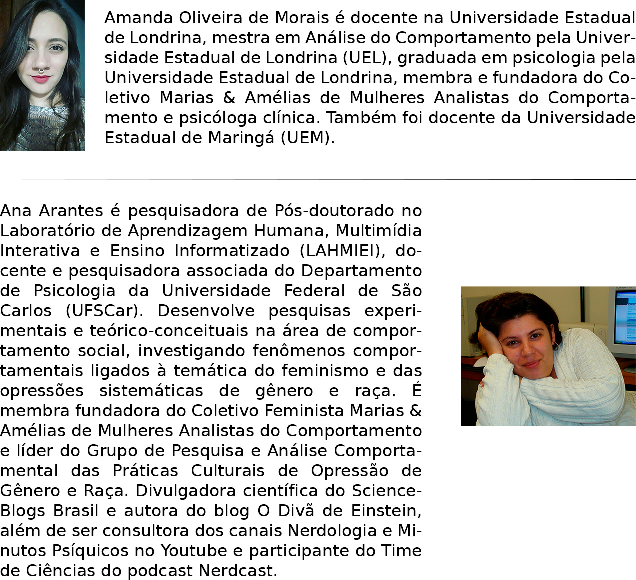
\includegraphics[scale=1]{autoras/autorasfinal1}\\
\newpage
\noindent
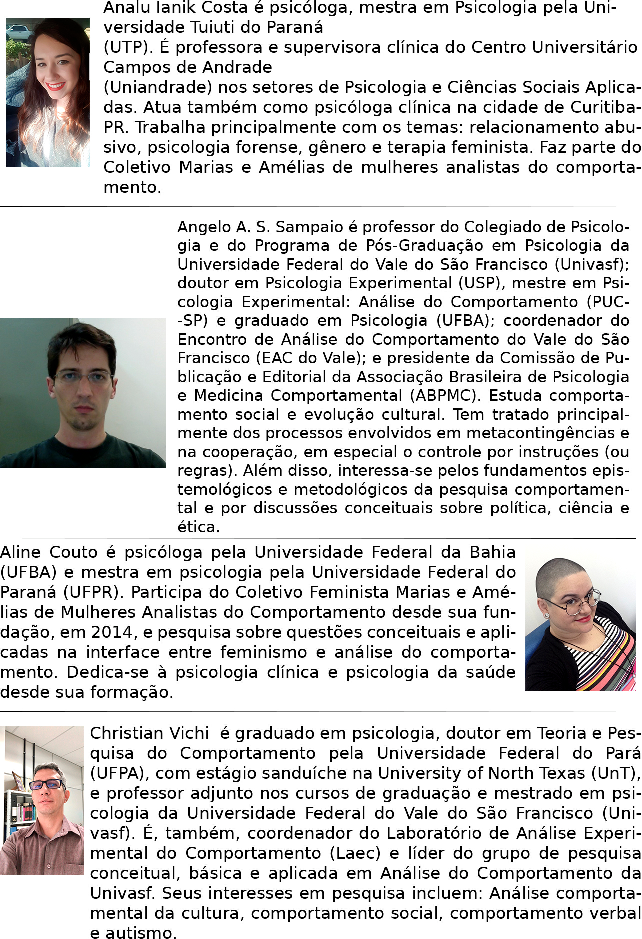
\includegraphics[scale=1]{autoras/autorasfinal2}
\chapter{Pioneiras: A história das primeiras mulheres na análise do comportamento no Brasil}\sectionmark{Pioneiras: A história das primeiras mulheres na análise do comportamento no Brasil}
\begin{flushright}
\begin{scriptsize}
Gabriela Jheniffer Teixeira Silva\footnote{Graduanda do curso de Psicologia da Universidade Federal de São Carlos.} \& Ana Arantes\footnote{Pesquisadora de Pós-doutorado do Programa de Pós-graduação em Psicologia (Comportamento e Cognição), docente e pesquisadora associada do Departamento de Psicologia da Universidade Federal de São Carlos.} \footnote{Este capítulo é proveniente da Monografia de Bacharelado da primeira autora, orientada pela segunda autora e apresentada ao Departamento de Psicologia da Universidade Federal de São Carlos (UFSCar) como uma das exigências para finalização do curso de graduação em Psicologia.}
\end{scriptsize}
\vspace{1cm}

\emph{De fato, eu me arriscaria a supor que Anônimo,\\
que escreveu tantos poemas sem assiná-los,\\
foi muitas vezes uma mulher.\\
(Virgínia Wolf, 1928)}
\end{flushright}

Pensar na ciência como um campo (majoritariamente) masculino não é algo recente. Pelo contrário, um dos primeiros estudos a abordar a diferença na produção científica entre homens e mulheres foi realizado por Rossi (1965). Apesar desse estudo ter sido conduzido há mais de 50 anos, seus resultados infelizmente podem ser facilmente extrapolados para este século. Mulheres tinham menor participação na produção científica em diversas áreas e, de acordo com a autora, isso poderia ser explicado pela falta de incentivo e desencorajamento sistemático, desde a idade escolar, para que mulheres se engajassem em atividades que não as preparassem para seu futuro ideal: ser esposa e mãe Rossi (1965). Historicamente, as mulheres foram domesticadas para, independentemente de sua formação, suas maiores conquistas serem um bom casamento e a criação de filhos (ver, por exemplo,  Rossi, 1965 e Foucault, 2003). Além disso, existia ainda uma restrição em aceitar mulheres em cursos do ensino superior, apoiada nos estereótipos acima citados (Nosik, 2018).

Apesar das mudanças relacionadas à aceitação e aos direitos conquistados na segunda metade do século XX e às lutas dos movimentos feministas em busca de igualdade entre homens e mulheres, ainda hoje, em pleno século XXI, são palpáveis as diferenças entre gêneros quanto ao acesso a riqueza, direitos e oportunidades (ONU, 2015, \textit{Minimum Set of Gender Indicators}). Para Bourdieu essas mudanças sociais não resolvem a questão da desigualdade pois:

\begin{quote}
(...) mesmo quando as pressões externas são abolidas e as liberdades formais – direito de voto, direito à educação, acesso a todas as profissões, inclusive políticas – são adquiridas, a autoexclusão e a ‘vocação’ (...) vêm substituir a exclusão expressa. (Bourdieu, 1998, p. 52, citado por Moraes, 2012)
\end{quote}

Ou seja, a crença de que homens e mulheres teriam mais chances de alcançar sucesso de acordo com suas supostas características e qualidades inerentes fundamenta e perpetua a disparidade entre gêneros em diversos âmbitos profissionais, incluindo a ciência (Souza \& Fonseca, 2008). Uma rápida análise histórica e cultural demonstra os diversos estigmas e consequentes dificuldades do ser mulher num campo que não fosse o papel tradicional: mãe, esposa e responsável pelas tarefas domésticas. De fato, as diferenças biológicas existem, mas em muitos casos elas se tornam a justificativa e não a causa das diferenças culturais. (Macêdo \& Macedo, 2004; Araújo, 2005; Moraes, 2012; e Da Silva, 2015).

Este movimento de exclusão e impedimento do envolvimento de mulheres na área científica pode ser definido como o \textit{silenciamento} e a \textit{invisibilização} feminina que acontecem dentro do contexto social considerado comum. O sujeito (ou grupo) coexiste em dimensões paralelas da realidade instituída, que ressignificam o \textit{ser humano} constantemente tendo como base as circunstâncias a que está submetido, englobando o trabalho, a política e a sexualidade. Essas variáveis seriam, então, cruciais para a construção não só do sujeito em si, mas da sua representação diante da sociedade (Da Silva, 2015). Como descrito pela autora, silenciamento e invisibilização explicitam os mecanismos pelos quais se marginalizam as minorias sociais:

\begin{quote}
O processo de silenciamento compõe a tríade: ausência de discurso, discurso como monólogo e discurso não considerado. Por sua vez, o processo de invisibilização estabelece a tríade: sujeito inconveniente, sujeito ignorado e o não-sujeito. (pp. 113-114)
\end{quote}

O silenciamento das mulheres na área científica ocorre pela ausência de discurso, por exemplo, quando não se criam condições para que mulheres sejam palestrantes em eventos científicos, pela falta de convite por parte dos organizadores ou pela imposição de exigências que impossibilitam que elas apresentem seus trabalhos (como a exigência de que palestras sejam proferidas apenas por Doutores, que impede que a maioria das mulheres, concentrada nos níveis de graduação e mestrado, tenha oportunidade de palestrar). O discurso como monólogo silencia as mulheres nas ciências, por exemplo, quando somos impedidas de expor pontos de vista particularmente femininos pelo fato de sermos obrigadas a seguir normatizações e procedimentos que limitam o discurso ao ponto de vista dominante e único dos homens, como a norma gramatical de se usar o pronome masculino como padrão.  Já o discurso não considerado silencia as mulheres em áreas científicas em que proposições femininas são diminuídas ou consideradas equivocadas pelo simples fato de serem emitidas por mulheres, o que pode ser visto, por exemplo, nas críticas infundadas à prática da terapia feminista como antiética, baseadas na noção de que existiria uma “ideologia feminista” que estaria sendo imposta ao cliente por parte da terapeuta. Em relação a tríade de invisibilização podemos compreender o sujeito inconveniente como aquele considerado indesejado pela sociedade, um incômodo que deve ser evitado e que é caracterizado, por exemplo, por regras não explícitas do tipo “pós-graduandas mulheres atrasam a defesa de seus projetos porque engravidam durante o curso”, que podem gerar preferência pela seleção de alunos homens por programas de pós-graduação, evitando-se a seleção de mulheres. O sujeito ignorado é aquele que, apesar de presente, não tem suas contribuições levadas em conta, exemplificado claramente pelo fenômeno do \textit{mansplaining}, em que mulheres, mesmo que com comprovada expertise em seus campos de atuação, são submetidas à situações em que homens explicam a elas os conceitos de suas especialidades de maneira condescendente e simplificada, ignorando que a mulher possa dominar o assunto em questão. E, por fim, o não-sujeito é aquele que sequer é considerado uma pessoa e passa a ser tratado como objeto, como coisa. Muitas vezes as mulheres são aceitas em laboratórios científicos não por suas contribuições intelectuais, mas por sua força de trabalho considerada meticulosa e perfeccionista, como se fossem equipamentos de pesquisa e não pesquisadoras.

Invisibilização e silenciamento podem ser observados também na associação automática que leitoras e leitores fazem ao se deparar com referências em artigos acadêmicos, feitas somente com o sobrenome da pessoa que escreveu o trabalho citado: se presume que autores de trabalhos acadêmicos são necessariamente do gênero masculino, mesmo em áreas predominantemente femininas, como a Psicologia, por exemplo. Outro caso parecido que podemos listar são os inúmeros feitos e pesquisas que foram realizados e/ou tiveram uma importante participação de mulheres cujos nomes são \textit{convenientemente} esquecidos. Não são apenas nomes ignorados, mas também e principalmente são histórias perdidas no tempo. Um dos casos mais emblemáticos é o de Rosalind Franklin. Foi a partir dos dados da pesquisa desta química britânica que foi possível elaborar o modelo de dupla hélice do DNA. Os dois cientistas – homens – que apresentaram tal descoberta para a comunidade científica foram gratificados com um Prêmio Nobel e, somente décadas depois, foi reconhecida a importância da participação de Franklin (Ortiz \& Silva, 2016). Outro caso que representa bem o machismo científico foi o de Nettie Stevens, uma das pioneiras no desenvolvimento de estudos genéticos que foram cruciais para a descoberta de que os determinantes do sexo de um organismo seriam cromossomos e não fatores ambientais. Apesar de um colega de laboratório ter chegado aos mesmos resultados tempos depois de Stevens, a descoberta foi creditada a ele, juntamente com o supervisor do laboratório em que trabalhavam (Lee, 2013).

Um estudo realizado por West, Jacquet, King, Correll e Bergstrom (2013) mostra que aproximadamente 70\% da produção científica mundial até o ano de 2012 era de autoria de homens. Para explicar esta disparidade existe um conceito cunhado por Rossiter (1993) denominado “Efeito Matilda” que descreve o sub-reconhecimento de cientistas do gênero feminino nas áreas acadêmicas por meio da invisibilização e apagamento de suas contribuições, como nos casos citados de Franklin e Stevens. As possíveis justificativas para este efeito são o fato das mulheres estarem mais propensas a deixar a academia por fatores pessoais, mais especificamente, devido ao acúmulo de jornadas de trabalho, resultado de uma distribuição ineficiente das responsabilidades domésticas. (Sousa \& Guedes, 2016). Esse desequilíbrio entre o trabalho e a vida pessoal interfere diretamente na produtividade e avanço destas cientistas. (Knobloch-Westerwick, Glynn, \& Huge, 2013). Outro fator apontado é a participação das mulheres em redes de colaboração: enquanto mulheres são mais propensas a colaborar com outros cientistas (independentemente de seu gênero), as redes de colaboração de homens têm como padrão ser composta quase exclusivamente por outros homens. Esses padrões na comunicação acadêmica podem ser cumulativos, levando a impossibilidade das mulheres acadêmicas se desenvolverem em suas carreiras (Knobloch-Westerwick et. al., 2013).

Rossi (1965) aponta possíveis caminhos para que uma sociedade e, consequentemente, uma ciência mais igualitária sejam alcançadas: 1. educar crianças de formas similares, para que papéis familiares e profissionais tenham o mesmo peso independente do gênero de quem os desempenha; e 2. entender que as possíveis dificuldades que uma mulher possa encontrar ao desempenhar uma profissão que exija mais dedicação não estão ligadas a sua (falta de) capacidade e sim ao acúmulo de papéis (esposa, mãe, profissional) e, a partir disso, compreender que isso é um problema social e histórico e não individual – atuando para que tal informação seja difundida e esta questão seja trabalhada em conjunto com a sociedade. Rossi (1965) aponta também que o aumento no número de mulheres cientistas seria uma das ferramentas para provocar as modificações coletivas necessárias para se alcançar a igualdade.

\section{Psicologia: Uma profissão feminina, mas uma ciência masculina}

Diante desse quadro de silenciamento das mulheres e de invisibilização da presença feminina no campo científico, não surpreende que, mesmo em áreas majoritariamente femininas, possamos verificar como as contribuições das mulheres são menos reconhecidas do que aquelas feitas por homens. Um caso emblemático a ser exemplificado é o das ciências psicológicas, cuja área (tanto acadêmica e científica, quanto aplicada) é formada por 90\% de profissionais mulheres, segundo levantamento do DIEESE (2016) sobre os dados da PNAD (Pesquisa Nacional por Amostra de Domicílio) realizada pelo IBGE (Instituto Brasileiro de Geografia e Estatística) em 2014.

A graduação em Psicologia, desde a sua fundação, foi composta por uma maioria esmagadora de mulheres (Rosemberg, 1984). Existem diversas variáveis que contribuem para a explicação desse fenômeno, como o possível reflexo dos modelos sexuais tradicionais (o que reservaria à mulher o papel de sentimental e “expressiva”), e a segregação ocupacional, que relega as mulheres profissões ligadas diretamente ao cuidado doméstico e com outras pessoas (Rosemberg, 1984). Essa presença expressiva das mulheres nas graduações em Psicologia não se traduz necessariamente em participação efetiva na construção da Psicologia como profissão e como corpo de conhecimento.  Dados recentes mostram que, no Brasil, há uma desproporção na presença de mulheres em relação à de homens conforme nos dirigimos à níveis mais altos da carreira. Por exemplo, as mulheres representam 90\% do total de profissionais de psicologia formadas e formados no país, mas a porcentagem de professoras mulheres cai drasticamente para 56,6\% dos professores de ensino superior em Psicologia (DIEESE, 2016).  Pensando na produção científica, mulheres são maioria desde a graduação até o nível do Pós-doutorado, mas coordenam apenas cerca de 40\% de grandes projetos de pesquisa (Costa, 2006). O que pode até soar relevante, no entanto, a autora aponta que, ainda que não exista um preconceito explícito, as estruturas sociais (família, religião, economia, direito, etc.) e a cultura agem “de forma a garantir a hegemonia masculina nos postos mais elevados das ciências” (p.458). Embora esses dados sejam sobre a participação feminina nas ciências em geral, e de não termos dados específicos sobre a participação feminina na Psicologia em particular, é de se esperar, considerando a literatura sobre invisibilização e silenciamento, que na nossa área essa tendência se repita.
\vfill

\section{Por que estudar a história da Análise do Comportamento no Brasil?}

Mesmo que não se tenha dados, específicos ou gerais, e estudos sobre a participação e contribuição das mulheres na ciência psicológica no Brasil, pensamos que um estudo sobre as desigualdades entre gêneros particularmente dentro da Análise do Comportamento (AC) pode servir como caso exemplar. A chegada da AC coincide com o desenvolvimento institucionalizado do curso de Psicologia no país, o que provavelmente é uma das razões para que tenha se tornado uma disciplina de currículo mínimo da graduação (Miranda \& Cirino, 2010) e colocado o Brasil entre os países em que a pesquisa científica na área seja uma das mais expressivas. 

Poucos anos após a vinda da AC para o Brasil, nos anos 1960, ocorreu o golpe militar. Tal fato impossibilitou um pleno desenvolvimento desta ciência naquele momento (Ferreira, 1985; Matos \& Carvalho, 1998). Ferreira (1985) afirma que cientistas brasileiros encontravam sérias limitações para o desenvolvimento da Psicologia como ciência por causa de um sistema de comunicação pobre entre os profissionais e por dificuldades econômicas do país que resultavam em cortes constantes de fundos para pesquisa e programas de graduação e pós-graduação descontinuados, chegando ao ponto de as próprias universidades não terem dinheiro suficiente para comprar livros e manter a assinatura de diversos periódicos. De acordo com Matos e Carvalho (1998), uma das principais dificuldades enfrentadas foi a falta de equipamentos e bibliografias necessários aqui no Brasil, o que também refletia diretamente na aprendizagem dos alunos. Durante a ditadura militar, os analistas do comportamento se viram obrigados, por conta das restrições pessoais, políticas e econômicas impostas, a voltar-se para a aplicação clínica e ensino. Houve diversos cancelamentos de viagens para o exterior, assim como dificuldades na importação de materiais e revogação de convites para professores de outros países virem ao Brasil por conta das restrições xenófobas impostas pelos militares (Todorov, 2004). 

Mesmo com este percalço, nem tudo foi perdido. Os trabalhos desenvolvidos na Universidade de Brasília (UnB) resultaram em publicações nacionais e internacionais significativas (Matos \& Carvalho, 1998). Além disso, por conta da dispersão dos profissionais pelo país, com o passar dos anos, muitos cursos de graduação em Psicologia tiveram em suas primeiras matrizes a influência direta do trabalho de Carolina Bori (Todorov \& Hanna, 2010). 

A constante produção de pesquisas em AC (básicas, aplicadas e conceituais) desde a década de 1960, a realização sistemática de diversos eventos científicos e o número crescente de periódicos e livros especializados são aspectos que fundamentam a importância de estudos históricos sobre a área no nosso país. Como destaca Cruz (2006), embora existam poucos exemplos de pesquisas históricas sobre a AC no Brasil, tais pesquisas podem ser instigantes e reveladoras e, principalmente, auxiliar no delineamento da produção de conhecimento na área. Apesar da pouca produção relativa a pesquisas históricas, nos últimos anos houve um aumento substancial de pesquisas voltadas para a análise histórico-conceitual, o que indica a consolidação da AC na comunidade científica, uma vez que a área se desenvolveu o suficiente para buscar, em sua história, aspectos relevantes que favorecem a identificação de fatores que estão constantemente afetando a constituição da AC e do Behaviorismo no Brasil (Cruz, 2006). 

\section{Presença e participação feminina na Análise do Comportamento brasileira}

No decorrer da história da AC no Brasil, diversas mulheres tiveram papéis importantes, algumas vezes até cruciais para o estabelecimento da área no país, mas pouco se tem registrado sobre suas contribuições. Um bom exemplo disso é o fato quase desconhecido de que o primeiro convite para que o Professor Keller\footnote{O Professor Fred S. Keller, em 1961, veio ao Brasil lecionar durante um ano como professor visitante na Universidade de São Paulo. No decorrer da disciplina de Psicologia Experimental, o Prof. Keller não só apresentava o conteúdo programático da AC, como administrava exercícios práticos em laboratório. Estas aulas foram a primeira semente da Análise Experimental do Comportamento no nosso país (Matos \& Carvalho, 1998).} viesse para o Brasil partiu de uma aluna do curso de Psicologia da Universidade de São Paulo, Mirtes Rodrigues do Prado (Couto, 2012). Uma das poucas mulheres com reconhecimento mais amplo dentro do campo da ciência psicológica foi a Professora Doutora Carolina Martuscelli Bori que, nas palavras de Matos e Carvalho (1998), conquistou este posto por “principalmente ao longo de várias gestões como parte da Diretoria da SBPC”, ter rompido “os tabus políticos mais resistentes deste país: uma mulher à frente dos cientistas brasileiros” (p.5).

Como já discutido, a invisibilização do trabalho feminino é histórica e não exclusiva do campo da Psicologia ou da AC – é uma opressão estrutural (Velho \& León 2012). Resgatar e trazer à tona o trabalho dessas mulheres é uma forma não só de resgatar ângulos não explorados da história da AC brasileira, como também de ir contra o movimento de apagamento dessa parte importante da história das mulheres que fazem e contribuem significativamente para a ciência. Por isso, neste estudo, pretendemos apresentar como a produção e a carreira acadêmico-científica dessas mulheres vem sendo retratada pela área e investigar o papel que a presença feminina teve na constituição e consolidação da AC no Brasil. Para esse objetivo realizamos um levantamento bibliográfico em nove bases de dados de periódicos científicos e em quatro periódicos nacionais da área de AC (como mostrado na Tabela 1), sem restrição de data, utilizando as seguintes combinações de buscadores: “início da Análise do Comportamento”, “história”, “Análise do Comportamento”, “Brasil”, “mulheres”, “behaviorismo”, e “pesquisa histórica”, bem como suas respectivas traduções para o inglês.

% Please add the following required packages to your document preamble:
% \usepackage{booktabs}
\begin{table}[]
\caption{Lista de bases de dados e periódicos da área de AC usados no levantamento bibliográfico.}
\begin{adjustbox}{max width=1\textwidth}
\begin{tabular}{@{}l@{}}
\toprule
\multicolumn{1}{c}{\textbf{Bases de dados}}                                     \\ \midrule
Biblioteca Nacional de Medicina dos Estados Unidos (PubMed)                     \\
Biblioteca Virtual em Saúde - Psicologia Brasil (Bvs-Psi)                       \\
Centro Latino-Americano e do Caribe de Informação em Ciências da	Saúde (Bireme) \\
\textit{Education Resources Information Center  (Eric)}                                  \\
Periódicos Eletrônicos em Psicologia (PEPsic)                                   \\
\textit{American Psychological Association (PsycInfo})                                   \\
\textit{Scientific	Electronic Library Online (Scielo) }                                  \\
\textit{SciVerse Scopus (Scopus)}                                                        \\
\textit{Web	of Science   }                                                               \\ \midrule
\multicolumn{1}{c}{\textbf{Periódicos nacionais de Análise do Comportamento}}   \\ \midrule
\textit{\textit{Acta Comportamentalia*}}                                                 \\
Revista Brasileira de Terapia Comportamental e Cognitiva (RBTCC)                \\
Revista Perspectivas em Análise do Comportamento                                \\
Revista Brasileira de Análise do Comportamento (REBAC)                          \\ \bottomrule
\end{tabular}
\end{adjustbox}
\caption*{*Apesar de ser um periódico internacional, os artigos selecionados neste periódico foram publicados em português, portanto optamos por incluí-lo na categoria de publicação nacional.}
\end{table}

Inicialmente, foram selecionados todos os artigos que continham um ou mais dos buscadores citados e aqueles que mostrassem uma ou mais palavras-chave semelhante aos buscadores utilizados.  A partir do título, resumo e, se necessário, a leitura completa do artigo, foram selecionados aqueles trabalhos que abordavam, por meio de estudos de caso ou históricos, os 20 primeiros anos da AC no Brasil e aqueles que continham informações históricas ou documentação sobre este período. Foram encontrados 2730 artigos e, destes, 16 foram selecionados seguindo os critérios descritos. 

A Figura 1.1 mostra a distribuição de artigos publicados por ano sobre a temática. Mesmo sem a existência de limitação de período temporal nas buscas, somente dois artigos foram publicados antes do ano 2000 e a maioria (nove dos 16 artigos) se concentra no período pós-2010. Esta informação corrobora o trabalho de Cruz (2006), comprovando a existência de uma lacuna a ser preenchida nesse âmbito, uma vez que existem poucas pesquisas históricas acerca da AC no país. 

\begin{figure}[h]
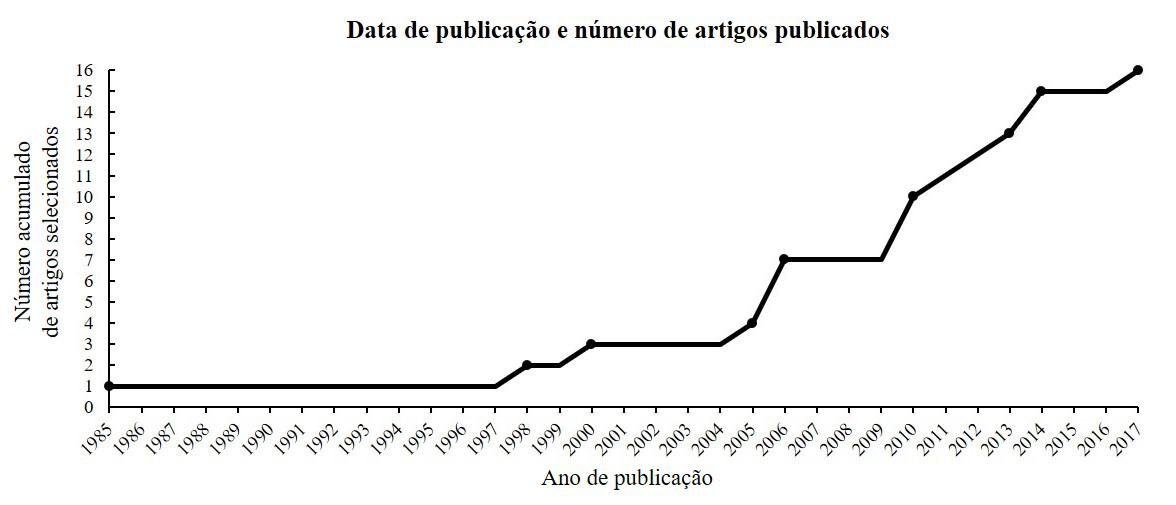
\includegraphics[width=1\textwidth]{1/figura1}
\captionof{figure}{Distribuição do número de artigos encontrados de acordo com as datas de publicação dos mesmos. A curva acumulada mostra o crescimento acelerado de publicações sobre história da AC a partir de 2010.}
\end{figure}

Ao se buscar um resgate histórico da construção de uma ciência, como no caso da AC, é crucial considerar que a relação entre o comportamento do cientista, a comunidade científica e o contexto cultural em que cientista e comunidade se inserem são aspectos indissociáveis. A complexidade e a amplitude dessas variáveis nos impossibilitam contar toda a história e estamos limitadas e limitados, de forma que qualquer tentativa de concretizar tal tarefa resulta em esboços da história. (Cruz, 2006). Tais esboços, entretanto, não perdem seu valor porque tornam possível identificar ao menos algumas das variáveis presentes na cultura daquele momento que se relacionam com o comportamento não só de uma cientista ou um cientista, mas de toda uma comunidade científica, de acordo com o contexto cultural e histórico (Cruz, 2006). Este capítulo é um exemplo de como podemos utilizar essas relações para recontar a história, estando nós mesmas inseridas num contexto diferente e analisar, com base nas informações atuais, como se deu a construção da AC para compreender como e por que se deu o apagamento sistemático de inúmeras histórias e contribuições de mulheres ao longo do desenvolvimento da área.

\begin{figure}
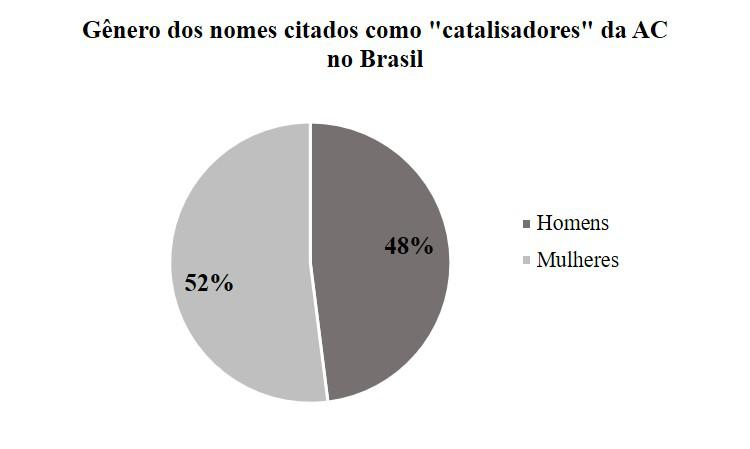
\includegraphics[width=1\textwidth]{1/figura2}
\captionof{figure}{Distribuição por gênero dos nomes da área de AC, citados nos artigos selecionados para o estudo, considerados “catalisadores” da AC no Brasil entre 1960 e 1985.}
\end{figure}

Os artigos selecionados na busca relatavam acontecimentos ocorridos entre 1960 e 1985, configurando os primeiros 25 anos da AC no país, e citavam um total de 55 nomes da pesquisa e da academia na área de AC e Behaviorismo Radical. Dentre esses, 29 eram mulheres, configurando 52\% do total, como podemos observar na Figura 1.2. A participação feminina no início da AC brasileira parece seguir a tendência expressa na Psicologia como um todo, demonstrada anteriormente, em que a participação das mulheres cai de 89\% de estudantes na graduação em Psicologia (Rosemberg, 1984) para uma participação de 56,6\% nos quadros docentes (DIEESE, 2016), e continua diminuindo para 52\% das pesquisadoras consideradas importantes para “catalisação” da AC. Pode parecer uma comparação entre desiguais, dado que se compara a porcentagem total de alunas de graduação nos cursos de Psicologia com a porcentagem de pesquisadoras cujos papéis dentro da área de AC são considerados fundantes. Porém, é de se pensar como os homens passam de 11\% dos estudantes de graduação em Psicologia daquela época (entre 1960 e 1980) para mais da metade dos grandes pesquisadores de uma ciência, enquanto a maioria das mulheres não ultrapassa os níveis da graduação e pós-graduação. Dado o contexto histórico do início da AC no Brasil, podemos buscar compreender esses dados como resultado dos papéis de gênero fortemente arraigados que desestimulavam então, e ainda desestimulam hoje, um maior envolvimento feminino profissional e acadêmico.

Mesmo com representação ligeiramente diminuída, relativamente à representação dos homens (29 mulheres para 26 homens citados), os números apresentados são importantes pois salientam que apesar de todo o contexto histórico envolvido, mulheres estiveram e foram presentes ativamente na formação de analistas do comportamento e na disseminação de laboratórios de Análise Experimental do Comportamento pelo país. Mostram também como a percepção do papel das mulheres na área é subestimado pelas próprias cientistas e pelos próprios cientistas, já que um levantamento informal entre colegas analistas do comportamento tende a mostrar que, além das Professoras Carolina Bori, Maria Amélia Matos e algumas outras, a maioria das pesquisadoras e dos pesquisadores de AC não tem informações sobre essa participação fundamental das mulheres na área.

Dentre os 16 artigos selecionados para este estudo, 62\% deles são de autoria estritamente masculina.  Esse dado é muito interessante se levarmos em consideração a discussão acerca do “Efeito Matilda” e como o gênero influencia nas escolhas de coautores: a maioria esmagadora dos artigos é escrita somente por homens e, em sua maioria, somente com outros homens como parceiros. Esse dado, aliado às informações já citadas da acerca da proporção de mulheres na Psicologia, nos mostra que esse efeito não acontece por falta de profissionais femininas nas áreas científicas, mas porque homens sistematicamente excluem as mulheres do fazer científico. Pode-se inferir, portanto, que é mais um exemplo prático do “Efeito Matilda”.

A representação das mulheres na AC vem sendo analisada há tempos no âmbito internacional. O trabalho de Poling et al. (1983) foi pioneiro desta área ao avaliar a contribuição das mulheres na produção científica da área no que diz respeito à autoria dos artigos publicados e na participação de mulheres nos conselhos editoriais dos principais periódicos internacionais. Esse estudo mostrou tendências crescentes na representação das mulheres como analistas do comportamento, ainda que essa participação não seja representativa do total de mulheres na área, em relação ao número relativo de homens. A pesquisa de Nosik (2018) mostra um aumento considerável da participação feminina na AC em diversas faixas etárias, o que demonstra que o aumento de cientistas mulheres é uma das ferramentas necessárias para promover mudanças de contingências necessárias para se alcançar a equidade, mesmo que os avanços sejam feitos aos poucos (Rossi, 1965).

Ao longo da leitura dos artigos selecionados para este estudo, percebemos que a participação feminina na formação da AC como área científica no Brasil se deu, principalmente, em três categorias de atuação distintas, ainda que sobrepostas em alguns casos: 1. a importância dessas profissionais no ensino da AC durante os anos iniciais da Psicologia no Brasil; 2. suas contribuições para o conhecimento analítico-comportamental nas áreas de pesquisa básica e aplicada; e 3. seu papel na difusão da AC como ciência e das tecnologias advindas desta. Desse modo, foi possível compreender de maneira mais acurada como se deram suas contribuições ao longo da formação da AC no país. A Tabela 1.2 mostra a distribuição das mulheres mencionadas nos artigos selecionados entre categorias formuladas. A atribuição das analistas do comportamento às categorias se deu seguindo os seguintes critérios:

\begin{enumerate}[1. ]
\item Contribuições Para o Ensino: quando, nos artigos selecionados, foram citadas informações acerca da carreira docente como Universidade, período de docência, disciplinas ministradas e afins.

\item Contribuições Científicas (Pesquisa): quando foram descritos o desenvolvimento ou estabelecimento de linhas de pesquisa e de laboratórios e/ou participação e orientação de alunos em laboratórios de pesquisa.

\item Contribuições Para a Difusão da AC: quando foram encontradas informações sobre a elaboração de livros para públicos diversos, participação na consolidação de políticas públicas, fundação ou participação em cursos de outras áreas (pedagogia, biologia, enfermagem etc), clínicas e institutos.
\end{enumerate}

% Please add the following required packages to your document preamble:
% \usepackage{booktabs}
% \usepackage{multirow}
\begin{table}[]
\caption{Categorização da participação feminina na formação da AC, segundo os artigos selecionados para o estudo.}
\begin{adjustbox}{max width=1\textwidth}
\begin{tabular}{@{}ccc@{}}
\toprule
\textbf{Categoria}                                                         & \textbf{Referência}                                           & \textbf{Analistas do comportamento citadas} \\ \midrule
\multicolumn{1}{c|}{\multirow{8}{*}{Ensino}}                               & \multicolumn{1}{c|}{\multirow{2}{*}{Barbosa et al., 2017}}    & Ana Lúcia Ulian                             \\
\multicolumn{1}{c|}{}                                                      & \multicolumn{1}{c|}{}                                         & Sandra Eli Bachiega                         \\ \cmidrule(l){2-3} 
\multicolumn{1}{c|}{}                                                      & \multicolumn{1}{c|}{\multirow{2}{*}{Miranda \& Cirino, 2010}} & Carolina Bori                               \\
\multicolumn{1}{c|}{}                                                      & \multicolumn{1}{c|}{}                                         & Maria Amélia Matos                          \\ \cmidrule(l){2-3} 
\multicolumn{1}{c|}{}                                                      & \multicolumn{1}{c|}{\multirow{4}{*}{Todorov \& Hanna, 2010}}  & Margarida Windholz                          \\
\multicolumn{1}{c|}{}                                                      & \multicolumn{1}{c|}{}                                         & Dora Fix Ventura                            \\
\multicolumn{1}{c|}{}                                                      & \multicolumn{1}{c|}{}                                         & Maria Inês Rocha e Silva                    \\
\multicolumn{1}{c|}{}                                                      & \multicolumn{1}{c|}{}                                         & Vera Konigsberger                           \\ \midrule
\multicolumn{1}{c|}{\multirow{10}{*}{Contribuição científica (Pesquisa)}}  & \multicolumn{1}{c|}{\multirow{6}{*}{Miranda \& Cirino, 2010}} & Maria Amélia Matos                          \\
\multicolumn{1}{c|}{}                                                      & \multicolumn{1}{c|}{}                                         & Dora Fix                                    \\
\multicolumn{1}{c|}{}                                                      & \multicolumn{1}{c|}{}                                         & Rachel Kerbauy                              \\
\multicolumn{1}{c|}{}                                                      & \multicolumn{1}{c|}{}                                         & Maria José Vasconsellos                     \\
\multicolumn{1}{c|}{}                                                      & \multicolumn{1}{c|}{}                                         & Adélia Teixeira                             \\
\multicolumn{1}{c|}{}                                                      & \multicolumn{1}{c|}{}                                         & Sonia dos Santos Castanheira                \\ \cmidrule(l){2-3} 
\multicolumn{1}{c|}{}                                                      & \multicolumn{1}{c|}{\multirow{3}{*}{Todorov \& Hanna, 2010}}  & Elenice Ferrari                             \\
\multicolumn{1}{c|}{}                                                      & \multicolumn{1}{c|}{}                                         & Deisy das Graças de Souza                   \\
\multicolumn{1}{c|}{}                                                      & \multicolumn{1}{c|}{}                                         & Herma Drachenberg                           \\ \cmidrule(l){2-3} 
\multicolumn{1}{c|}{}                                                      & \multicolumn{1}{c|}{Fidalgo, 2014}                            & Carolina Bori                               \\ \midrule
\multicolumn{1}{c|}{\multirow{16}{*}{Difusão da Análise do Comportamento}} & \multicolumn{1}{c|}{\multirow{2}{*}{Miranda \& Cirino, 2010}} & Carolina Bori                               \\
\multicolumn{1}{c|}{}                                                      & \multicolumn{1}{c|}{}                                         & Maria Amélia Matos                          \\ \cmidrule(l){2-3} 
\multicolumn{1}{c|}{}                                                      & \multicolumn{1}{c|}{Todorov \& Hanna, 2010}                   & Maria Helena Leite Hunziker                 \\ \cmidrule(l){2-3} 
\multicolumn{1}{c|}{}                                                      & \multicolumn{1}{c|}{Polanco, 2014}                            & Ione Scarpelli Pereira                      \\ \cmidrule(l){2-3} 
\multicolumn{1}{c|}{}                                                      & \multicolumn{1}{c|}{\multirow{12}{*}{Barbosa et al., 2017}}   & Mercedes Cunha de Carvalho                  \\
\multicolumn{1}{c|}{}                                                      & \multicolumn{1}{c|}{}                                         & Marilena Ristum                             \\
\multicolumn{1}{c|}{}                                                      & \multicolumn{1}{c|}{}                                         & Márcia Bonagamba                            \\
\multicolumn{1}{c|}{}                                                      & \multicolumn{1}{c|}{}                                         & Vera Otero                                  \\
\multicolumn{1}{c|}{}                                                      & \multicolumn{1}{c|}{}                                         & Marlene Gonzales                            \\
\multicolumn{1}{c|}{}                                                      & \multicolumn{1}{c|}{}                                         & Anamélia Araújo de Carvalho                 \\
\multicolumn{1}{c|}{}                                                      & \multicolumn{1}{c|}{}                                         & Ana Cecília Sousa Bittencourt Bastos        \\
\multicolumn{1}{c|}{}                                                      & \multicolumn{1}{c|}{}                                         & Ana Helena Galvão                           \\
\multicolumn{1}{c|}{}                                                      & \multicolumn{1}{c|}{}                                         & Márcia Miriam Gomes                         \\
\multicolumn{1}{c|}{}                                                      & \multicolumn{1}{c|}{}                                         & Liana Sodré                                 \\
\multicolumn{1}{c|}{}                                                      & \multicolumn{1}{c|}{}                                         & Zorilda Goes                                \\
\multicolumn{1}{c|}{}                                                      & \multicolumn{1}{c|}{}                                         & Profa. Luzidéia*                           
\end{tabular}
\end{adjustbox}
\caption*{*Não há informações sobre o nome completo dessa analista do comportamento.}
\end{table}

De um total de 29 mulheres citadas como “catalisadoras” e pioneiras da consolidação da AC no Brasil, quatro dos 16 artigos selecionados apresenta a maioria das mulheres (16 citadas) na categoria de Difusão da Análise do Comportamento, novamente seguindo a tendência, verificada tanto em outras áreas da Psicologia quanto dentro da AC, da presença feminina mais expressiva nas áreas aplicadas (ou seja, na prestação de serviços psicológicos) do que nas áreas científicas. Nas categorias de Contribuição Científica (Pesquisa) e de Ensino foram alocadas 10 e oito analistas do comportamento, respectivamente. Nota-se, também, que as Professoras Carolina Bori e Maria Amélia Matos aparecem nas três categorias, atestando sua importância para a AC brasileira. A Professora Dora Fix Ventura tem seu papel categorizado, também, tanto em Contribuição Científica (Pesquisa) como em Ensino. Em contraste com esse reconhecimento da área a essas pesquisadoras e professoras, temos o nome da Professora Luzidéia, citada no artigo de Barbosa, Costa, Ulian e Lima (2017), sobre a qual não encontramos maiores informações, nem mesmo sobre seu nome completo. O fato de essa professora ser somente citada em um estudo sobre a AC no Nordeste, região historicamente negligenciada nas políticas educacionais e científicas do país, não nos foge à atenção.

Para uma melhor visualização e entendimento do desenvolvimento da AC no Brasil através das contribuições das mulheres da área, foi elaborada uma linha do tempo com as informações coletadas nos artigos selecionados, mostrada na Tabela 1.3. Podemos ver, nessa cronologia, a expressiva participação das mulheres desde o lançamento das bases experimentais da AC no Brasil, com a fundação de laboratórios experimentais e intercâmbio com pesquisadores internacionais já estabelecidos, passando pelo ensino de disciplinas de Análise Experimental do Comportamento e outras disciplinas de Psicologia sob a ótica analítico-comportamental, até o início da clínica comportamental, estabelecendo a área aplicada e a prestação de serviços em Análise do Comportamento Aplicada.
\vfill
\pagebreak

\scriptsize
% Please add the following required packages to your document preamble:
% \usepackage{booktabs}
% \usepackage{longtable}
% Note: It may be necessary to compile the document several times to get a multi-page table to line up properly
\begin{longtable}{@{}ccc@{}}
\caption{Linha do tempo das participações e contribuições das mulheres analistas do comportamento nos primeiros 20 anos da AC no Brasil, conforme descrito nos artigos selecionados para este estudo.}\\
\toprule
\textbf{Período} & \textbf{Participação das analistas do comportamento}                                                                                                                                                                                                                                                                                                                                                                                                                                                                                                                                                                                                    & \textbf{Referências}                                                                         \\* \midrule
\endhead
%
1960-1970        & \begin{tabular}[c]{@{}c@{}}Deisy das Graças de Souza, então bolsista\\ de iniciação científica, Elenice Ferrari e outros estudantes\\ desenvolvem pesquisas sobre controle aversivo,\\ reconhecidas por sua qualidade e originalidade\\ e publicadas em revistas internacionais.\end{tabular}                                                                                                                                                                                                                                                                                                                                                           & Todorov \& Hanna, 2010                                                                       \\* \midrule
1961             & \begin{tabular}[c]{@{}c@{}}Maria Amélia Matos, Dora Fix Ventura,\\ Margarida Windholz, Vera Konigsberger e\\ Maria Inês Rocha e Silva são as primeiras alunas\\ do curso oferecido por Keller durante sua\\ primeira vinda ao Brasil.\end{tabular}                                                                                                                                                                                                                                                                                                                                                                                                      & Todorov \& Hanna, 2010                                                                       \\* \midrule
1961-1962        & \begin{tabular}[c]{@{}c@{}}Maria Amélia Matos e Carolina Bori trabalham\\ como assistentes do professor Keller.\\ Foram responsáveis pelo primeiro\\ laboratório de AC no Brasil.\end{tabular}                                                                                                                                                                                                                                                                                                                                                                                                                                                          & Cirino, 2012                                                                                 \\* \midrule
1962             & \begin{tabular}[c]{@{}c@{}}Bori se torna uma das primeiras professoras de\\ Psicologia do curso de Pedagogia da Faculdade de Filosofia, \\ Ciências e Letras da cidade de Rio Claro, interior de SP. \\ \\ Herma Drachenberg, sob supervisão de Carolina Bori,\\ esenvolve em conjunto com outro cientista\\ um protótipo do \textit{Personalized System of Instruction} \\ (PSI, da sigla em inglês para Sistema Personalizado de Ensino)\end{tabular}                                                                                                                                                                                                          & Todorov \& Hanna, 2010                                                                       \\* \midrule
1963-1964        & \begin{tabular}[c]{@{}c@{}}Carolina Bori lidera a formação do Departamento\\ de Psicologia da Universidade de Brasília (UnB).\end{tabular}                                                                                                                                                                                                                                                                                                                                                                                                                                                                                                              & Cirino, 2012                                                                                 \\* \midrule
1965             & \begin{tabular}[c]{@{}c@{}}Maria Helena Leite Hunziker e outro cientista\\ fundam o primeiro centro voltado para\\ formação de AC da cidade de Campinas-SP.\end{tabular}                                                                                                                                                                                                                                                                                                                                                                                                                                                                                & Hanna \& Todorov, 2010                                                                       \\* \midrule
1968             & \begin{tabular}[c]{@{}c@{}}Criação do curso de Psicologia na\\ Universidade Federal da Bahia.\\ Profa. Mercedes Cunha de Carvalho é uma das\\ principais colaboradoras, participando da elaboração\\ da grade curricular.\end{tabular}                                                                                                                                                                                                                                                                                                                                                                                                                  & Barbosa et al., 2017                                                                         \\* \midrule
1969             & \begin{tabular}[c]{@{}c@{}}Carolina Bori ministra um curso que versa sobre\\ Psicologia Social Experimental, considerado\\ marco para o início da AC na Universidade\\ Federal de Minas Gerais (UFMG). \\ \\ Ione Scarpelli Pereira, então professora da UFMG,\end{tabular}                                                                                                                                                                                                                                                                                                                                                                             & \begin{tabular}[c]{@{}c@{}}Miranda \& Cirino, 2010\\ \\ \\ Polanco, 2014\end{tabular}        \\* \midrule
1969-1971        & \begin{tabular}[c]{@{}c@{}}Bori ministra aulas no programa de pós-graduação\\  em Psicologia Experimental da USP.\\ \\ Alguns dos principais trabalhos em AC no início\\ da década de 1970 são orientados por Bori. \\ \\ Maria Amélia Matos é responsável por montar\\ o laboratório de comportamento operante,\\ trazendo material dos EUA para a UFMG. \\ \\ Dora Fix coordena o Laboratório\\ de Psicologia Sensorial da UFMG.\\ Carolina Bori e Maria Amélia Matos recebem\\ professores de outras universidades interessados em AC\\ (intercâmbio entre UFMG e USP-São Paulo)\end{tabular}                                                        & \begin{tabular}[c]{@{}c@{}}Miranda \& Cirino, 2010\\ \\ \\ Nale, 1998\end{tabular}           \\* \midrule
1969-1979        & \begin{tabular}[c]{@{}c@{}}Todas as pesquisas sobre comportamento\\ verbal produzidas neste período\\ (totalizando seis estudos) são orientadas\\ por Carolina Bori – enquanto professora da USP.\end{tabular}                                                                                                                                                                                                                                                                                                                                                                                                                                          & Fidalgo, 2014                                                                                \\* \midrule
1970             & \begin{tabular}[c]{@{}c@{}}Rachel Kerbauy escreve o manual “Análise Experimental\\ do Comportamento: exercícios de laboratório”,\\ utilizado amplamente no desenvolvimento do laboratório\\ de AC na UFMG. Seus métodos foram minuciosamente\\ seguidos por discentes e docentes. Maria José Vasconcellos e\\ Sonia Castanheira atuam neste laboratório\\ \\ (Uma curiosidade: o primeiro laboratório de pombos da UFMG\\ foi montado dentro de um dos banheiros do departamento.)\end{tabular}                                                                                                                                                         & \begin{tabular}[c]{@{}c@{}}Miranda \& Cirino, 2010\\ \\ \\ Polanco, 2014\end{tabular}        \\* \midrule
1970-1971        & \begin{tabular}[c]{@{}c@{}}Sonia Santos Castanheira, graduada em Psicologia\\ pela UFMG, que se tornara professora da mesma\\ universidade nos anos 60, inicia pesquisas em AC\\ envolvendo pombos no laboratório didático.\end{tabular}                                                                                                                                                                                                                                                                                                                                                                                                                & Cirino, 2012                                                                                 \\* \midrule
1971             & \begin{tabular}[c]{@{}c@{}}Redação do Regulamento do Laboratório de Psicologia\\ da UFMG, documento assinado por\\ Sonia dos Santos Castanheira.\\ \\ Carolina Bori auxilia na instalação do\\ laboratório de Psicologia Experimental da\\ Universidade Federal do Maranhão (UFMA).\\ Na época foram contratadas duas psicólogas\\ recém-formadas para ministrar aulas:\\ Marilena Ristum e Márcia Bonagamba.\end{tabular}                                                                                                                                                                                                                              & \begin{tabular}[c]{@{}c@{}}Miranda \& Cirino, 2010\\ \\ \\ Barbosa et al., 2017\end{tabular} \\* \midrule
1971-1972        & \begin{tabular}[c]{@{}c@{}}As docentes Maria José Vasconsellos e Maria Amélia Matos\\ são responsáveis pelo I Encontro de Psicologia Experimental\\ na Faculdade de Filosofia e Ciências Humanas da UFMG.\end{tabular}                                                                                                                                                                                                                                                                                                                                                                                                                                  & Miranda \& Cirino, 2010                                                                      \\* \midrule
1972             & \begin{tabular}[c]{@{}c@{}}Vera Otero e Marlene Gonzales substituem\\ Ristum e Bonagamba em seu trabalho na UFMA.\end{tabular}                                                                                                                                                                                                                                                                                                                                                                                                                                                                                                                          & Barbosa et al., 2017                                                                         \\* \midrule
1973             & \begin{tabular}[c]{@{}c@{}}Anamélia Araújo de Carvalho assume a coordenação\\ do Laboratório e o ensino de Psicologia Experimental da \\ Universidade Federal da Bahia (UFBA),\\ junto com algumas egressas como\\ Ana Cecília Sousa Bittencourt Bastos, Ana Helena Galvão,\\ Márcia Miriam Gomes, dentre outras.\\ Este grupo é o primeiro a exercer profissionalmente a\\ terapia comportamental em Salvador-BA.\end{tabular}                                                                                                                                                                                                                         & Barbosa et al., 2017                                                                         \\* \midrule
1974             & \begin{tabular}[c]{@{}c@{}}Adélia Teixeira é orientanda de\\ Doutorado de Bori na USP-SP.\end{tabular}                                                                                                                                                                                                                                                                                                                                                                                                                                                                                                                                                  & Miranda \& Cirino, 2010                                                                      \\* \midrule
1979             & \begin{tabular}[c]{@{}c@{}}Ana Lúcia Ulian, formada pela\\ Universidade de Londrina(UEL) juntamente com\\ Liana Sodré e Zorilda Goes integraram o grupo de\\ ensino da disciplina de Psicologia Experimental da UFBA.\end{tabular}                                                                                                                                                                                                                                                                                                                                                                                                                      & Barbosa et al., 2017                                                                         \\* \midrule
1984             & \begin{tabular}[c]{@{}c@{}}Ana Lúcia Ulian assume a coordenação do\\ Laboratório e as disciplinas de\\ \\ Psicologia Experimental 1 e 2 da UFBA\\ (trabalhos que reveza com outro professor).\\ Estas disciplinas propunham um programa que\\ se utilizava de artigos com conteúdo clínico e\\ metodologia experimental.\\ \\ Posteriormente faz parte do quadro de supervisores\\ do Estágio em Clínica da mesma universidade.\\ É fundado o segundo curso de Psicologia na\\ Universidade de Fortaleza (UNIFOR).\\ \\ \\ As disciplinas de AC são ministradas pela\\ Profa. Luzidéia, ex-aluna da\\ Universidade Federal do Ceará (UFC).\end{tabular} & Barbosa et al., 2017                                                                         \\* \midrule
1985             & \begin{tabular}[c]{@{}c@{}}A Profa. Sandra Eli Bachiega é contratada\\ pela UFC e se torna responsável por supervisões\\ na área clínica utilizando terapia comportamental.\end{tabular}                                                                                                                                                                                                                                                                                                                                                                                                                                                                & Barbosa et al., 2017                                                                         \\* \bottomrule
\end{longtable}
\normalsize
\vfill
\pagebreak

\section{Considerações Finais}
A invisibilização e o silenciamento das mulheres no contexto científico têm sido mostrados em diversos estudos das áreas de Sociologia, Antropologia e História, desde o impedimento inicial da participação feminina nas universidades, até o completo apagamento das cientistas responsáveis por descobertas críticas para a evolução científica em seus campos. Na Psicologia de modo geral, e na AC em particular, esse cenário não é diferente, porém a AC tem progressivamente reparado essa desigualdade histórica reconhecendo aos poucos o papel das mulheres pioneiras da área na fundação da ciência e da prestação de serviços em AC no país, muito por iniciativa das próprias pesquisadoras, como este estudo atesta. 

Para uma melhor compreensão das variáveis históricas e sociais implicadas nas práticas culturais de silenciamento e invisibilização das mulheres na sociedade e na ciência é preciso que tenhamos informações mais precisas sobre a presença e a participação feminina, com dados demográficos específicos sobre o número de mulheres nas associações da área, sua participação nos congressos, nas publicações e nos vários campos de aplicação da AC. McSweeney, Donahoe e Swindell (2000) sugerem a aplicação e acompanhamento de estatísticas formais sobre a participação de mulheres e minorias na AC como uma das estratégias para buscar a equidade da produção e do acesso à academia. Dessa forma, teremos um quadro mais preciso da situação de desigualdade entre os gêneros dentro da área, primeiro passo para a proposição de intervenções para modificar os sistemas de opressão de gênero. E, assim como Nosik (2018), encorajamos as futuras pesquisadoras e os futuros pesquisadores a continuar investigando as variáveis ambientais e práticas culturais de desigualdade de gênero e seus impactos, em prol de uma ciência analítico-comportamental mais igualitária.

Por fim, uma observação deve ser feita a respeito do conceito de \textit{mulher} utilizado neste estudo: partimos do princípio da distinção de categorias de gênero (feminino e masculino) socialmente construídas, de acordo com teóricas feministas como Rubin (1975) e Lerner (1986), e analistas do comportamento feministas como Ruiz (2003)\footnote{Para maiores discussões sobre o conceito de gênero e as considerações analítico-comportamentais feitas a partir dele, ver o capítulo ?? neste livro.}. Entretanto, é importante levar em consideração que a categoria \textit{mulher} não é única e sim múltipla (Esmeraldo, 2006). Variáveis como raça, orientação sexual, identidade de gênero e classe social das analistas do comportamento pioneiras citadas neste estudo não foram levadas em consideração por falta destas informações em documentos históricos e nos artigos encontrados. Sabe-se, no entanto, que o perfil da população com nível universitário nas décadas de 1960 a 1980, no Brasil, era de homens brancos, heterossexuais e cisgêneros (ao menos publicamente), originários das classes sociais mais altas (Ristoff, 2014). Tendo em vista este contexto histórico-cultural, pode-se inferir que a maioria - para não dizer a totalidade - das mulheres citadas aqui se enquadrem nos mesmos padrões de raça, orientação sexual e identidade de gênero públicas, além de compartilharem da mesma classe social. Tais interseccionalidades são frequentemente negligenciadas, portanto é necessária a realização de pesquisas que foquem em tais recortes para que possamos vislumbrar os seus impactos na construção da ciência. Nomes, histórias e contribuições foram e continuam sendo apagadas de forma recorrente – e o caso das mulheres é o mais evidente.

\chapter*{Referências Bibliográficas}\sectionmark{Referências Bibliográficas}
\hangindent=25pt
\hangafter=1
\noindent Araújo, M. F. (2005). Diferença e igualdade nas relações de gênero: Revisitando o debate. \textit{Psicologia Clínica}, 17(2), 41-52.

\hangindent=25pt
\hangafter=1
\noindent Barbosa, J. I. C., Costa, N., Ulian, A. L. A. O, \& Lima, L. S. (2017). Memórias da Análise do Comportamento no Nordeste: Bahia, Ceará e Maranhão. \textit{Revista Brasileira de Terapia Comportamental e Cognitiva}, 19, 61-70.

\hangindent=25pt
\hangafter=1
\noindent Camargo, W. X., \& Kessler, C. S. (2017). Além do masculino/feminino: Gênero, sexualidade, tecnologia e performance no esporte sob perspectiva crítica. \textit{Horizontes Antropológicos}, 47, 191-225.

\hangindent=25pt
\hangafter=1
\noindent Costa, M. C. (2006). Ainda somos poucas: Exclusão e invisibilidade na ciência. \textit{Cadernos Pagu,} 27, 455-459.
 
\hangindent=25pt
\hangafter=1
\noindent Couto, A. (2012). História da Análise do Comportamento no Brasil. \textit{Revista Online Comporte-se: Psicologia e Análise do Comportamento}.  Retirado de: http://www.comportese.com/2012/02/historia-da-analise-do-comportamento-no-brasil/

\hangindent=25pt
\hangafter=1
\noindent Cruz, R. N. (2006). História e Historiografia da Ciência: considerações para pesquisa histórica em análise do comportamento. \textit{Revista Brasileira de Terapia Comportamental e Cognitiva}, 8(2), 161-178. 

\hangindent=25pt
\hangafter=1
\noindent Departamento Intersindical de Estatísticas e Estudos Socioeconômicos. (2016). Levantamento de informações sobre a inserção dos psicólogos no mercado de trabalho brasileiro. Retirado de: \url{http://bit.ly/dieese2016}

\hangindent=25pt
\hangafter=1
\noindent Esmeraldo, G. G. S. L. (2006). O feminismo no plural: Para pensar a diversidade constitutiva das mulheres.\textit{ Revista Estudos Feministas,} 14(3), 829-831.

\hangindent=25pt
\hangafter=1
\noindent Ferreira, M. C. R. (1985). The study of behavioural development in Brazil: Contemporary research, teaching, and practice. \textit{International Journal of Behavioral Development}, 8, 139-151.

\hangindent=25pt
\hangafter=1
\noindent Ferreira, M. C. (2004). Sexismo hostil e benevolente: Inter-relações e diferenças de gênero. \textit{Temas em Psicologia,} 12(2), 119-126.

\hangindent=25pt
\hangafter=1
\noindent Foucault, M. (2003). História da Sexualidade, Volume 1: A vontade de saber. Rio de Janeiro: Graal. (Trabalho original publicado em 1988).

\hangindent=25pt
\hangafter=1
\noindent Knobloch-Westerwick, S., Glynn, C. J., \& Huge, M. (2013). The Matilda effect in science communication: An experiment on gender bias in publication quality perceptions and collaboration interest. \textit{Science Communication,} 35(5), 603-625.

\hangindent=25pt
\hangafter=1
\noindent Lee, J. J. (2013). Six women scientists who were snubbed due to sexism. \textit{National Geographic}. Retirado de: \url{http://bit.ly/leejj2013}

\hangindent=25pt
\hangafter=1
\noindent Lerner, G. (1986). The Creation of Patriarchy. New York: Oxford University Press.

\hangindent=25pt
\hangafter=1
\noindent Macêdo, G. S., \& Macedo, K. B. (2004). As relações de gênero no contexto organizacional: O discurso de homens e mulheres. \textit{Revista Psicologia Organizações e Trabalho}, 4(1), 61-90. 

\hangindent=25pt
\hangafter=1
\noindent Matos, M. A., \& Carvalho, A. M. A. (1998). Carolina Martuscelli Bori: Uma cientista brasileira. \textit{Psicologia: Reflexão e Crítica}, 11(2), 411-420. 
 
\hangindent=25pt
\hangafter=1
\noindent McSweeney, F. K., Donahoe, P., \& Swindell, S. (2000). Women in applied behavior analysis. \textit{The Behavior Analyst}, 23(2), 267-277.

\hangindent=25pt
\hangafter=1
\noindent Miranda, R. L., \& Cirino, S. D. (2010). Os primeiros anos dos laboratórios de análise do comportamento no Brasil. \textit{Psychologia Latina}, 1(1), 79-87.

\hangindent=25pt
\hangafter=1
\noindent Moraes, E. (2012). Ser mulher na atualidade: A representação discursiva da identidade feminina em quadros humorísticos de Maitena. Em I. Tasso \& P. Navarro, (Orgs.), \textit{Produção de identidades e processos de subjetivação em práticas discursivas}, (pp. 259-285). Maringá: Eduem.

\hangindent=25pt
\hangafter=1
\noindent Nosik, M. R., Luke, M. M., \& Carr, J. E. (2018). Representation of women in Behavior Analysis: An empirical analysis. \textit{Behavior Analysis: Research and Practice}, 1(2), 1-9.

\hangindent=25pt
\hangafter=1
\noindent Organização das Nações Unidas. (2015). Minimum Set of Gender Indicators. Disponível em https://genderstats.un.org

\hangindent=25pt
\hangafter=1
\noindent Ortiz, E., \& Silva, M.R. (2016). O uso de abordagens da História da Ciência no ensino de biologia: Uma proposta para trabalhar a participação da cientista Rosalind Franklin na construção do modelo da dupla hélice do DNA. \textit{Investigações em Ensino de Ciências}, 21(1), 106-123. 

\hangindent=25pt
\hangafter=1
\noindent Poling, A., Grossett, D., Fulton, B., Roy, S., Beechler, S., \& Wittkopp, C. J. (1983). Participation by women in behavior analysis.\textit{ The Behavior Analyst,} 6, 145-152.

\hangindent=25pt
\hangafter=1
\noindent Ristoff, D. (2014). O novo perfil do campus brasileiro: Uma análise do perfil socioeconômico do estudante de graduação. \textit{Avaliação: Revista da Avaliação da Educação Superior} (Campinas), 19(3), 723-747.

\hangindent=25pt
\hangafter=1
\noindent Rosemberg, F. (1984). Afinal, por que somos tantas psicólogas? \textit{Psicologia: Ciência e Profissão}, 4(1), 6-12. 

\hangindent=25pt
\hangafter=1
\noindent Rossi, A. (2012). Women in science: Why so few? \textit{Science}, 148(3674), 1196-1202.

\hangindent=25pt
\hangafter=1
\noindent Rossiter, M. W. (1993). The Matthew Matilda effect in science. \textit{Social Studies of Science}, 23(2), 325-341. 

\hangindent=25pt
\hangafter=1
\noindent Rubin, G. (1975). The traffic in women. Em: R. Reiter, (Org.), \textit{Towards an Antropology of Women}, (pp. 160-207). New York: Monthly Review Press. 

\hangindent=25pt
\hangafter=1
\noindent Ruiz, M. R. (2003). Inconspicuous sources of behavioral control: The case of gendered practices. \textit{The Behavior Analyst Today}, 4, 12–16. 

\hangindent=25pt
\hangafter=1
\noindent Da Silva, W.A. (2015). Foucault e indigenciação: As formas de silenciamento e invisibilização dos sujeitos. \textit{Problemata: Revista Internacional de Filosofia}, 6(3), 111-128. 

\hangindent=25pt
\hangafter=1
\noindent Sousa, L. P., \& Guedes, D. R. (2016). A desigual divisão sexual do trabalho: Um olhar sobre a última década. \textit{Estudos Avançados,} 30(87), 123-139. 

\hangindent=25pt
\hangafter=1
\noindent Souza, M. R. F., \& Fonseca, M. C. F. R. (2008). Mulheres, homens e matemática: Uma leitura a partir dos dados do Indicador Nacional de Alfabetismo Funcional. Educação e Pesquisa, 34(3), 511-526. 

\hangindent=25pt
\hangafter=1
\noindent Todorov, J. C., \& Hanna, E. S. (2010). Análise do Comportamento no Brasil. \textit{Psicologia: Teoria e Pesquisa}, 26(SpE), 143-154.

\hangindent=25pt
\hangafter=1
\noindent Todorov, J. C. (2004). Da aplysia à constituição: Evolução de conceitos na análise do comportamento. \textit{Psicologia: Reflexão e Crítica}, 17(2), 151-156.

\hangindent=25pt
\hangafter=1
\noindent Velho, L., \& León, E. (2012). A construção social da produção científica por mulheres. \textit{Cadernos Pagu}, 10, 309-344. 

\hangindent=25pt
\hangafter=1
\noindent Woolf, V. (1985). Um teto todo seu. Rio de Janeiro: Nova Fronteira. (Trabalho original publicado em 1928.)

\hangindent=25pt
\hangafter=1
\noindent West, J. D., Jacquet, J., King, M. M., Correll, S. J., \& Bergstrom, C. T. (2013). \textit{The role of gender in scholarly authorship}. PloS ONE, 8(7), e66212.
\chapter*{Pontes entre o feminismo interseccional e a análise do comportamento}\sectionmark{Pontes entre o feminismo interseccional e a análise do comportamento}
\addcontentsline{toc}{chapter}{Capítulo 2}
\addcontentsline{toc}{section}{Pontes entre o feminismo interseccional e a análise do \\comportamento}
\addcontentsline{toc}{subsection}{\textbf{Autora:} \textit{Táhcita Medrado Mizael}}
\begin{flushright}
\begin{small}
    Táhcita Medrado Mizael    
\end{small}
\vspace{1cm}
\end{flushright}

O feminismo pode ser conceituado, grosso modo, como um movimento de luta pela conquista de direitos iguais entre os homens e as mulheres. Ele costuma ser dividido em três grandes ondas, a primeira da metade do século XIX até os anos 1960, a segunda entre a década de 1960 e os anos 1980, e por fim, a terceira, da década de 1980 até os anos atuais (e.g., Nogueira, 2017). Em resumo, as pautas das lutas na primeira onda envolveram o desejo de emancipação das mulheres, as quais eram dependentes e subordinadas a seus maridos, além da reivindicação de direitos que apenas os homens tinham, como o direito de votar. 

Na segunda onda, com o início da participação das mulheres brancas de classe média e alta no mercado de trabalho, uma pauta bastante presente foi o reconhecimento da opressão sobre as mulheres, especialmente na família nuclear e no trabalho. Em 1949, com a publicação de ``O segundo sexo'', de Simone de Beauvoir, muitas mulheres utilizaram o livro como inspiração para as lutas ao reconhecerem que elas eram consideradas menos cidadãs que seus parceiros homens. Nesse contexto, a frase ``não se nasce mulher, torna-se'' ficou internacionalmente famosa, sendo utilizada como base para a divisão entre o sexo designado no nascimento – vinculado ao aparato biológico e, portanto, considerado natural, dos homens e mulheres – e o gênero (masculino e feminino) – caráter social das diferenças sexuais entre homens e mulheres, algo considerado construído e não natural (e.g., Piscitelli, 2002; Scott, 1995).

Um slogan nessa fase que ficou muito famoso foi ``O pessoal é político'', utilizado para evidenciar que qualquer tipo de violência ocorrida no âmbito familiar não deveria ser ocultado; pelo contrário, as violências deveriam ser expostas para que a vítima pudesse ser ajudada e o perpetrador, responsabilizado. Outras pautas presentes foram a defesa do direito à contracepção e ao aborto, questionamentos envolvendo a sexualidade, como a existência da heterossexualidade compulsória (Rich, 1980/2010) e a objeção ao tratamento das mulheres como objetos na publicidade, na pornografia e também nas artes (e.g., Nogueira, 2017; Schiebinger, 2008). 

O leitor mais crítico pode, desde o início do texto, ter se perguntado sobre quais mulheres e quais homens foram referidos até o momento, uma vez que homens e mulheres negras eram obrigados a trabalhar em condições sub-humanas e sem poder exercer uma série de direitos que as pessoas brancas tinham, como o direito de estudar. Além disso, para uma variedade de pessoas (como as mulheres lésbicas, homens negros, indivíduos portadores de deficiências, pessoas que moram no campo, etc.), seus marcadores sociais (características físicas e/ou simbólicas) as colocam em diferentes posições. Sendo assim, suas reivindicações seriam diferentes, por terem uma vida distinta da maioria das mulheres que ``protagonizaram'' (por terem condições de fazê-lo) os feminismos mais conhecidos. 

Foi na segunda onda também que o feminismo negro surgiu com mais força, denunciando que as demandas e reivindicações existentes até o momento no feminismo eram pautadas na experiência de mulheres brancas, ocidentais e da classe média. Um relato muito importante, ainda no período da primeira onda, foi o de Sojourner Truth, na Convenção dos Direitos das Mulheres ocorrida em 1851, que denunciava naquela época os perigos da essencialização da categoria ``mulher'': 

\begin{quote}
    Aquele homem lá diz que uma mulher precisa ser ajudada ao entrar em carruagens, e levantada sobre as valas, e ficar nos melhores lugares onde quer que vá. Ninguém me ajuda em lugar nenhum! E eu não sou uma mulher? Olhem para mim! Olhem para o meu braço. Eu arei, eu plantei e eu recolhi tudo para os celeiros. E nenhum homem pode me auxiliar. E eu não sou uma mulher? Eu poderia trabalhar tanto e comer tanto quanto qualquer homem (...) e suportar o chicote tão bem quanto! E eu não sou uma mulher? Eu dei à luz a crianças e vi a maior parte delas ser vendida como escravas. E quando eu chorei com o sofrimento de uma mãe, ninguém além de Jesus me ouviu. E eu não sou uma mulher? (Brah \& Phoenix, 2004, p. 77).
\end{quote}

A terceira onda do feminismo é marcada por uma diversidade e pluralidade de pensamentos e posicionamentos, com destaque para 1) o feminismo pós-moderno e pós-estruturalista (e.g., Butler, 2003), que questiona a existência de uma identidade coerente e estável; 2) a presença de posições teóricas que problematizam concepções feministas essencialistas (e.g, Butler, 2001; Louro, 2008) e 3) críticas com relação a separação de sexo e gênero, com o primeiro considerado uma diferença natural e o segundo, artificial/construído (e.g., Nicholson, 2000), uma vez que não existe sexo pré-discursivo (Butler, 2003), além de críticas com relação a concepções monolíticas da subjetividade. Assim, a desconstrução, a diversidade e a fragmentação identitária são características bastante presentes na terceira onda.

Assim, o feminismo, ou melhor, os feminismos não são movimentos monolíticos ou homogêneos. Sua divisão em ondas tampouco é acurada, uma vez que pode dar a impressão errônea de que as ideias surgiram em um mesmo momento e foram substituídas por novas demandas, sem que as demandas antigas subexistissem ou que houvesse pontos discordantes nos discursos das feministas. Além disso, é importante frisar que as demandas reivindicadas nessas três ondas consistiam, sumariamente, das demandas de mulheres brancas da classe média, muitas delas estadunidenses (Piscitelli, 2002; Nogueira, 2017).
\vfill

\section*{Epistemologia feminista e críticas à concepção de ciência moderna}\sectionmark{Epistemologia feminista e críticas à concepção de ciência moderna}

Pelo menos desde a década de 1970, muitas feministas, especialmente as acadêmicas, começaram a criticar as concepções de ciência correntes. Elas perceberam uma relação entre os conhecimentos científicos produzidos e problemas centrais do movimento, como a subordinação das mulheres em diversos âmbitos. As feministas criticaram fortemente o uso do masculino como universal, a exclusão das mulheres como pesquisadoras e a subordinação destas como objeto de pesquisa, o enviesamento androcêntrico e as lacunas e generalizações nas pesquisas (Schiebinger, 2008). Como exemplo tem-se as pesquisas sobre ansiedade e depressão. A maioria dos estudos sobre modelos animais é feito com ratos machos, e os ensaios clínicos com homens. Os resultados, contudo, são generalizados para toda a população. Além disso, durante muitos anos houve uma naturalização das diferenças entre os sexos como produtos biológicos (e.g., a inteligência, habilidades viso-espaciais e a coordenação motora foram consideradas habilidades que somente os homens tinham, apesar de haver dados mostrando que essas habilidades são aprendidas). No entanto, hoje sabe-se que meninos muitas vezes desenvolvem mais as habilidades de raciocínio viso-espacial e coordenação motora fina, por exemplo, pela exposição a brinquedos os quais as meninas são proibidas e/ou punidas ao brincar (e.g., Porto, 2016; Schiebinger, 2008).

Até mesmo campanhas de saúde veiculadas televisivamente são focadas no masculino. Pense em quais são os sintomas de infarto do miocárdio. Dor no peito, náuseas, suor frio e desmaios, certo? Na verdade, nas mulheres muitos sintomas do infarto do miocárdio são diferentes e envolvem, por exemplo, falta de ar, cansaço inexplicável e arritmia (\textit{National Institute of Health}, 2012). Além disso, a representação do óvulo e espermatozoide como agentes passivo e ativo, respectivamente, em livros didáticos, vídeos e outros tipos de mídia também é incorreta (e.g., Keller, 2006).

Com base nas diversas críticas à concepção de ciência corrente na época, algumas epistemologias feministas foram desenvolvidas, com posições que variavam desde as mais liberais até as mais radicais. Nas posições mais liberais, há certa concordância com os pressupostos da ciência moderna e o foco é em pesquisas sobre questões que dizem mais respeito às mulheres. Assim, as feministas que adotam as posições mais liberais consideram que a ciência é neutra e desinteressada, que conhecedor e conhecido estão separados, que a ciência pode ser objetiva, etc., mas que é necessário focar os estudos nas experiências das mulheres. Por outro lado, as posições mais radicais vão questionar inclusive a objetividade e a racionalidade como bases da metodologia científica, evidenciando que a ciência está imbrincada na política e na ideologia, ou seja, que é impossível um pesquisador ser neutro e seus interesses e/ou pesquisas, desinteressadas. (Nogueira, 2017).

Assim, por exemplo, no empiricismo feminista, parte-se de uma concepção na qual é possível corrigir os vieses androcêntricos e sexistas se as regras da pesquisa científica forem cumpridas à risca. Para as teorias de \textit{standpoint} feministas (e.g., Harding, 1986), por outro lado, além de seguir as normas da pesquisa científica de maneira estrita, é necessário que se pesquisem sobre as mulheres, suas experiências e concepções sobre os acontecimentos. Por fim, uma terceira epistemologia feminista vai advogar a recusa a qualquer discurso universalizante, fomentando a existência de conhecimentos situados, ou seja, que uma pesquisa realizada em determinado local e contexto pode ter (e provavelmente terá) resultados distintos da mesma pesquisa realizada em outro local e/ou contexto. As duas primeiras abordagens, portanto, possuem uma concepção universal e generalizante da mulher, essencializando-a, que é justamente o que a terceira abordagem busca evitar.

\section*{Interseccionalidades}\sectionmark{Interseccionalidades}

O termo interseccionalidade tem sido utilizado em uma variedade de contextos, sendo considerado um método de pesquisa, uma teoria, uma abordagem, um paradigma, um conceito, uma metáfora analítica, entre outros (e.g., Davis, 2008). Historicamente, o estudo das interseccionalidades foi fortemente influenciado pelo feminismo negro, ou seja, um dos movimentos feministas nos quais as mulheres negras perceberam que a intersecção entre diferentes marcadores sociais, especialmente raça e gênero, dificultava sua identificação com as lutas feministas (principalmente nas décadas de 1960 a 1980) e com as lutas pelos direitos civis. O relato de Falcón (2009) ilustra isso:

\begin{quote}
    As ativistas mulheres de cor dessa época eram frequentemente forçadas a optar por um dos lados entre as lutas feministas e as dos direitos civis. Fazer a escolha era difícil para mulheres de cor porque suas experiências não eram apenas baseadas em raça \textit{ou} gênero, mas em raça e gênero. Frustradas com feministas brancas que fracassaram em integrar o antirracismo em seu ativismo e com homens de cor que fracassaram na luta contra seu sexismo, as mulheres de cor começaram a se organizar e vocalizar suas questões [específicas] (Falcón, 2009, p. 467, itálicos adicionados).
\end{quote}

Assim, o termo \textit{feminismo interseccional} tem sido utilizado para denominar feminismos nos quais as interseccionalidades são levadas em consideração nas análises, ou seja, que ser mulher pode produzir formas de opressão, mas que essa característica não é (ou não deveria ser) considerada a única ou a mais importante forma de opressão. 

O primeiro registro do termo interseccionalidade foi feito pela pesquisadora estadunidense Kimberlé Crenshaw em 1989, para se referir à abordagem que leva em consideração a interação entre diversas formas de subordinação. A Teoria da Interseccionalidade (TI) parte de um questionamento relacionado aos feminismos mais ``tradicionais'', que abordavam, entre outras coisas, as diferenças de gênero, no sentido de masculino/feminino. Nesse sentido, em vez de pesquisar as diferenças entre homens e mulheres, a TI ressalta a importância de se pesquisar também as diferenças entre as próprias mulheres. O objetivo de tal empreitada é reduzir os essencialismos, ao descentrar os discursos dominantes focados, primordialmente, nas diferenças entre homens e mulheres brancos e de classe média de sociedades ocidentais (Henning, 2015; Nogueira, 2017).

Para a TI, todo conhecimento é considerado 1) socialmente construído e 2) parcial e limitado histórica ou politicamente. Além disso, a TI enfatiza a importância de coexistirem uma variedade de posições, indicando, portanto, que os posicionamentos de determinado indivíduo dependem de sua história de vida, dos contextos aos quais ele foi exposto e das experiências que teve. Desse modo, diferentes marcadores sociais são dotados de diferentes valorações em diferentes contextos, o que expõe o caráter relacional de aspectos e características humanas. Na TI, o foco de análise é a interação ou intersecção entre as várias categorias ou identidades a qual uma pessoa pertence (marcadores sociais), como raça, sexo designado no nascimento, identidade de gênero, orientação sexual, deficiências, classe, idade/geração, território, nacionalidade, corporalidade, etc. (Aguião, 2015; Nogueira, 2017; Piscitelli, 2008). Para Crenshaw (2002):

\begin{quote}
    A interseccionalidade é uma conceituação do problema que busca capturar as consequências estruturais e dinâmicas da interação entre dois ou mais eixos de subordinação. Ela trata especificamente da forma pela qual o racismo, o patriarcalismo, a opressão de classe e outros sistemas discriminatórios criam desigualdades básicas que estruturam as posições relativas de mulheres, raças, etnias, classes e outras (p. 177).
\end{quote}

Assim, diferentemente de concepções mais tradicionais, onde predomina o raciocínio de que os marcadores sociais se somam, essa teoria\footnote{De acordo com Adriana Piscitelli (2008), existem duas abordagens predominantes sobre as interseccionalidades: a abordagem sistêmica e a abordagem construcionista. Em termos gerais, na primeira abordagem, há um foco sobre o caráter repressivo dos marcadores sociais na possibilidade de agência (capacidade de identificar relações de controle – geralmente aversivo – e agir, de modo a reduzir o controle aversivo) das mulheres, e o segundo possui uma concepção de dinamismo maior, de modo que a articulação entre os diferentes marcadores sociais pode gerar contextos de opressão, mas também de agência para as mulheres. Este texto utiliza a segunda abordagem do termo.} mostra que a articulação destes marcadores cria condições de opressão e privilégio, dependendo dos contextos onde os indivíduos estão e da própria articulação entre os marcadores. 

Diante da pergunta ``quem tem mais desvantagem: homens ou mulheres?'', a resposta pode variar a depender dos outros marcadores incluídos na análise. São homens e mulheres brancos? Eles vivem na cidade, no campo? São jovens, idosos? E se for um homem negro e uma lésbica branca? Existem pesquisas mostrando, inclusive, que certas palavras que deveriam ser utilizadas para descrever homens e mulheres, como ``\textit{Black}'' (negro), e até palavras que descrevem uma classe de pessoas (``\textit{women}'', mulheres), independente de outros atributos evocam respostas muito especificas. No caso, \textit{Black} evoca a classe ``homens negros'' apenas, e \textit{women}, ``mulheres brancas'' (e.g., Goff, Jackson, Di Leone, Culotta, \& DiTomasso, 2014; Steinbugler, Press, \& Dias, 2006; Warner, 2008). Nas palavras de Warner (2008), ``um estereótipo diferente é eliciado quando gênero e raça são considerados juntos, do que quando raça ou gênero são considerados sozinhos'' (Warner, 2008, p. 457).

\section*{É possível uma articulação entre o feminismo (interseccional) e a análise do comportamento?}\sectionmark{É possível uma articulação entre o feminismo (interseccional) e a análise do comportamento?}

O feminismo interseccional pode ser conceituado como a análise das formas de entrelaçamento entre diferentes marcadores sociais contextualizados histórica e culturalmente que podem produzir desigualdades, mas também formas de resistência e/ou privilégios. Ele ``se opõe à ideia de partir de diferenças tidas como relevantes \textit{à priori}'' (Henning, 2015, p. 110)

Pressupostos feministas são coerentes com a abordagem analítico-comportamental e contribuições da análise do comportamento (AC) para os feminismos foram realizadas, principalmente pela pesquisadora Maria Ruiz (Ruiz, 1995, 1998, 2003, 2009; 2013; Ruiz \& Roche, 2007), mas também por outros (e.g., Couto \& Dittrich, 2017; Fideles \& Vandenberghe, 2014; Silva \& Laurenti, 2016). Em seguida, serão apontadas algumas das críticas aos modelos de ciência feitos por feministas, seguidas por explicações analítico-comportamentais (parte da discussão a seguir pode ser vista em alguns dos estudos supracitados): 


\begin{enumerate}
    \item Visão contextual e subjetiva do conhecimento científico: 
\end{enumerate}   
Uma crítica comum no discurso feminista em geral, ou seja, de várias abordagens feministas, como apontado por Ruiz (1995), é a suposição de que o conhecimento científico é objetivo e neutro e de que conhecedor e conhecido estão separados. Desde a década de 1970, alguns feminismos defendem uma ciência na qual o cientista não pode ser separado do objeto a ser conhecido, uma vez que este faz parte do mesmo ambiente. Nesse sentido, o conhecimento científico não pode ser neutro nem objetivo, uma vez que as realidades são construídas socialmente (e.g., Schiebinger, 2008). A AC possui uma visão que concorda (pelo menos parcialmente) com o pressuposto de que todo conhecimento é contextual e subjetivo. Nas palavras de Skinner (1974):

\begin{quote}
    Seria absurdo para o behaviorista afirmar que está de alguma forma isento de sua análise. Ele não pode sair do fluxo causal e observar o comportamento de algum ponto de vista especial [...]. No próprio ato de analisar o comportamento humano, ele está se comportando – como no próprio ato de analisar o pensamento, o filósofo está pensando (p. 234; tradução da autora).
\end{quote}

\begin{enumerate}[resume]
    \item Visão contextualista de mundo
\end{enumerate} 

Outra crítica presente no discurso feminista apontada por Ruiz\linebreak (1995) e especialmente dirigida à psicologia, é que esta é individualizante, uma vez que os problemas psicológicos, apesar de serem pautados em contextos sócio-políticos, são considerados pela psicologia como questões individuais. Exemplos disso são a violência doméstica, em que é comum ver análises da vítima e do agressor sem levar em consideração os contextos mais amplos no qual a agressão ocorreu, o ``indivíduo ansioso'' ou ``depressivo'', diagnosticado e tratado individualmente, sem considerar porque a pessoa desenvolveu tais transtornos; e o preconceito racial, onde o indivíduo ``racista'' é considerado o problema a ser tratado, como se o racismo viesse ou fosse uma propriedade de instâncias internas e não fosse aprendido no ambiente no qual o indivíduo está inserido. 

Diferentemente de algumas abordagens psicológicas consideradas individualizantes, e em concordância com o discurso feminista que\linebreak preza por análises contextuais, a AC possui uma visão contextualista de mundo, onde os contextos históricos e imediatos são fundamentais para a análise. Em uma pesquisa sobre violência doméstica de Bernard Guerin e Marcela Ortolan (2017), por exemplo, os autores apontam que a análise de um ou mais episódios de violência contra a mulher requer não só a análise do comportamento do par, mas também do ambiente mais abrangente. Isto envolve, segundo os autores, os contextos políticos, históricos, sociais e econômicos atuais, os quais oferecem, muitas vezes, condições para que diversos tipos de violência sejam reforçados e/ou naturalizados. 

\begin{enumerate}[resume]
    \item Agência como uma forma de controle recíproco sobre as contingências ambientais
\end{enumerate}

No discurso feminista, agência é um termo utilizado para se referir, grosso modo, à capacidade de identificar relações de controle (geralmente aversivo) e buscar formas de eliminar ou reduzir o controle aversivo. Assim, uma terceira crítica das feministas parte do entendimento de que a agência é algo externo ao indivíduo (e não uma relação organismo-ambiente, como a AC a entende) e que, portanto, é impossível modificar práticas opressivas se ``não tenho'' ou ``não possuo'' agência. Entretanto, para a AC, o conceito de agência diz respeito a um controle recíproco sobre contingências ambientais (Ruiz, 1998), de modo que o ambiente causa mudanças em nosso comportamento, mas nós também modificamos o ambiente: ``os homens agem sobre o mundo, modificam-no e, por sua vez, são modificados pelas consequências de suas ações'' (Skinner, 1957/1978, p. 15). Nesse sentido, é possível que a concepção de agência utilizada nos feminismos seja coerente com a proposta analítico-comportamental, sendo vista como uma forma de autoconhecimento que instrumentaliza o indivíduo para a ação.

Após verificar, portanto, que vários pressupostos dos feminismos são coerentes com a proposta analítico-comportamental, de que maneira nossas ferramentas ou formas de análise podem auxiliar no estudo das diferenças entre homens e mulheres (e entre as próprias mulheres e os próprios homens)?

Ruiz (2003) faz uma análise do que ela chama de práticas culturais generificadas, mostrando que o sexo designado no nascimento dos indivíduos serve como estímulo discriminativo para tais práticas. Assim, por exemplo, temos evidência de que professores de ensino fundamental reforçam classes de respostas de seus alunos diferencialmente, dependendo do sexo da criança: se o indivíduo é um menino, a qualidade do trabalho é reforçada. Se for menina, por outro lado, a aparência do trabalho é reforçada. Tal reforço diferencial é dado em uma série de contextos e com relação a uma variedade de respostas, como a maneira de se sentar, o que é considerado bagunça, que tipos de interesses são reforçados (matemática para os meninos e artes para as meninas), etc. 

Outro exemplo se refere ao comportamento assertivo. Segundo Del Prette e Del Prette (2005), na ``base do conceito de assertividade encontra-se a noção de igualdade de direitos e deveres, de legitimidade dos comportamentos voltados para a reivindicação e defesa desses direitos, de respeito e dignidade da pessoa humana.'' (p.175). Entretanto, é comum ver no dia a dia que uma mesma classe de respostas emitidas por homens e mulheres que poderia levar o rótulo de assertividade é considerada assertiva somente quando emitida por homens; as mesmas respostas emitidas por mulheres são consideradas ``agressivas''.

Assim, em resumo, para Ruiz (2003):

\begin{quote}
    Quando nós falamos de práticas culturais generificadas, nós estamos falando de formas de controle social relacionadas ao poder e a relações de dominância que levam diretamente ao nível de acesso que um indivíduo ou grupo de indivíduos podem ter a fontes de reforçamento ou alocação de recursos (p. 15; tradução da autora).
\end{quote}

E o feminismo interseccional? Apesar de várias dessas contribuições serem possíveis em vários tipos de feminismos, de que maneira a AC poderia contribuir especificamente no feminismo interseccional?

\begin{enumerate}
    \item Concepção de que todo conhecimento é socialmente construído:
\end{enumerate}

A TI e o feminismo interseccional adotam a concepção de que as formas de conhecimento são socialmente construídas. Para a AC, a concepção de conhecimento presente nas propostas construcionistas sociais se refere ao ``saber que'' (\textit{knowing that}), ou seja, ``conhecer significa comportar-se com o comportamento verbal apropriado'' (Guerin, 1992/2009, p. 5). Guerin (1992/2009) relaciona a AC e algumas abordagens construcionistas utilizando duas abordagens principais modernas: a de Gergen e Davis (1985) e a de Moscovici (1988).

Para Gergen e Davis (1985) existem quatro concepções presentes no construcionismo social: 1) a de que ``nossas relações com o mundo nem sempre correspondem ao mundo real'' (Guerin, 1992/2009, p. 3), com a implicação de que mesmo que essas relações e objetos sejam inventados/criados, tais relações podem influenciar o comportamento aberto e encoberto dos indivíduos; 2) a concepção de que a forma com a qual explicamos o mundo (pelo uso da linguagem) também se configura como um produto social; 3) a concepção de que a manutenção de qualquer conhecimento não depende de sua validade empírica, mas de sua relação com o ambiente social e não social; e 4) de que conhecimentos construídos socialmente são inseparáveis de nossas vidas sociais e se relacionam com várias outras atividades sociais. Além disso, para Gergen e Davis (1985), conhecimento não é uma propriedade ou um objeto existente na cabeça das pessoas, mas coisas que as pessoas fazem juntas, o que também é coerente com a proposta analítico-comportamental.

Outros pesquisadores da AC também têm evidenciado pontos de contato entre a AC e o construcionismo social. Roche e Barnes-Holmes (2003), por exemplo, relataram semelhanças (e diferenças) entre a proposta construcionista social e a proposta analítico-comportamental: 1) a natureza do conhecimento: ambas as abordagens consideram que o conhecimento científico possui origem social e seu entendimento se baseia no estudo de práticas da comunidade verbal; 2) a linguagem como peça-chave para a ação humana: a concepção de que a linguagem é uma convenção social e o interesse em análises funcionais da linguagem, e 3) ênfase no contexto e história para analisar os eventos, para citar apenas três. 

A proposta analítico-comportamental compartilha a noção de que as formas pelas quais compreendemos o mundo são o produto do ambiente social ao qual os indivíduos pertencem. Descrições do mundo e do próprio \textit{self}, são, portanto, resultado de um processo de aprendizagem de relações complexas formadas no contato com o mundo, de maneira que nossas concepções sobre o mundo, sobre quem somos e o que sentimos não correspondem a uma realidade objetiva, mas sim a uma série de aprendizagens sociais. 

Do mesmo modo, a linguagem, ou melhor, os significados que damos aos vários aspectos da linguagem (símbolos, gestos, verbalizações, etc.) são determinados e compartilhados por uma comunidade verbal social, ou seja, uma mesma palavra (símbolo ou gesto) pode ter diferentes significados em diferentes culturas, ou ainda dentro de uma mesma cultura (ou comunidade verbal). Assim, é possível considerar a AC como uma abordagem construcionista social que converge com a concepção presente nas abordagens interseccionais (e, consequentemente, no feminismo interseccional) de que conhecimentos são socialmente construídos. 

\begin{enumerate}[resume]
    \item Identificação de relações de controle
\end{enumerate}

A descrição operacional das contingências, prática básica da AC, pode ser muito útil na identificação e descrição acurada das complexas relações envolvidas nos eventos de interesse do universo do feminismo interseccional. Resgatando a pergunta ``quem sofre mais violência no Brasil: Homens ou mulheres?'', possíveis relações de controle seriam: o primeiro indivíduo pode responder sob controle da violência que ocorre nas ruas. A segunda pode responder sob controle da violência doméstica, e uma terceira relação de controle estaria baseada nos dados de violência policial. Portanto, o tipo de violência (física, psicológica, etc.), o contexto no qual a pessoa sofreu a violência, quem a perpetrou, entre outros, são variáveis que podem controlar a emissão da resposta e, portanto, criar diferentes verdades ou concepções sobre o assunto.

A identificação de relações de controle também se relaciona com outro aspecto central da TI e do feminismo interseccional, que é a oposição à ideia de partir de diferenças consideradas relevantes à priori, ou seja, antes da análise. Os contextos vão ``informar'' quais diferenças, marcadores sociais e/ou outros estímulos controlaram as respostas que determinado indivíduo emitiu em determinado evento. 

\begin{enumerate}[resume]
    \item Ênfase no aspecto relacional e na história dos indivíduos
\end{enumerate}

Na seção sobre ``Interseccionalidades'', foi ressaltada a descoberta, em algumas pesquisas, de que certas palavras que são utilizadas para descrever homens e mulheres podem evocar respostas específicas, como no caso de ``\textit{Black}'', geralmente assumido como ``homem negro'', e ``woman'' como ``mulher branca'' (e.g., Warner, 2008). Essa descoberta pode ser analisada, em nosso referencial, a partir de um modelo recente, elaborado no contexto da teoria das molduras relacionais\footnote{A teoria das molduras relacionais é uma abordagem moderna da linguagem e cognição humanas. De acordo com essa teoria, a base da cognição e linguagem humana está na habilidade de aprender diferentes tipos de relações entre estímulos, de modo que a aprendizagem de algumas relações seja suficiente para que um indivíduo derive outras relações, ou seja, aprenda algumas relações sem que seja instruído para fazê-lo. Para saber mais, consulte Hayes et al. (2001).} (\textit{Relational Frame Theory}, RFT, em inglês; Hayes, Barnes-Holmes \& Roche, 2001).

O nome desse modelo é DAARE, \textit{Differential Arbitrarily Applicable Relational Responding Effects} (efeitos do responder relacional diferencial arbitrariamente aplicado) e ele surgiu em um contexto de pesquisa na qual os experimentadores tiveram dificuldade em explicar porque alguns estímulos se relacionavam mais entre si do que outros. Especificamente, em uma tarefa na qual os participantes tinham que relacionar cores com cores, cores com formas e formas com formas, os experimentadores verificaram que os participantes tinham mais facilidade em relacionar ``cor-cor'' do que ``forma-forma'' (Finn, Barnes-Holmes, Hussey, \& Graddy, 2016). O que os pesquisadores hipotetizaram, em um estudo subsequente (Finn, Barnes-Holmes, \& McEnteggart, 2018), é que talvez esses resultados ocorreram porque, na história verbal com essas palavras, a frequência de emissão das palavras utilizadas na pesquisa que se referiam a cores era maior que a frequência de emissão de palavras que denotavam formas. Para este modelo, então, essa frequência diferencial no uso das palavras referentes às cores e às formas evoca mais respostas de orientação às primeiras, em comparação com as segundas, de modo que há uma maior coerência, isto é, uma maior consistência entre o padrão de responder relacional e a história comportamental que deu origem a esse padrão nas relações ``cor-cor'' do que nas relações ``forma-forma''. 

Neste contexto, pesquisas podem se utilizar desse modelo para discutir resultados já encontrados na literatura, por exemplo: sobre vieses raciais e de gênero, na criação de novas pesquisas que investiguem esses efeitos e aplicando-os a questões como estereótipos de gênero e a intersecção gênero-raça. O estudo de Barnes-Holmes, Murphy, Barnes-Holmes e Stewart (2010), por exemplo, investigou a existência de vieses raciais implícitos em participantes adultos. Os participantes tinham que responder a relações consideradas consistentes ou inconsistentes com suas histórias de vida, respondendo verdadeiro ou falso às relações ``homem branco carregando armas-seguro'', ``homem branco carregando armas-perigoso'', ``homem negro carregando armas-seguro'' e ``homem negro carregando armas-perigoso''. Veja que, além da história verbal com esses estímulos, existe também a história do responder a ``verdadeiro'' ou ``falso'', com o primeiro ocorrendo em uma frequência maior que o segundo (a frequência de emissão da resposta ``verdadeiro'' tende a ser maior que a frequência de emissão da resposta ``falso''). 

Nesse estudo, a hipótese era que, de acordo com as respectivas histórias de vidas, os participantes responderiam com uma rapidez semelhante às relações entre homens negros e perigo e a homens brancos e segurança. Entretanto, os resultados mostraram que os participantes tiveram mais facilidade em relacionar ``branco-seguro'' do que ``negro-perigoso''. De acordo com o modelo DAARE, e como interpretado por Barnes-Holmes, Harte e McEnteggart (no prelo), se a foto do homem branco e a palavra ``seguro'' tiverem funções avaliativas positivas para os participantes, ao passo que a foto do homem negro e a palavra ``perigoso'' tivessem funções avaliativas negativas, é possível interpretar tais resultados em termos de maior ou menor coerência entre ``branco-seguro-verdadeiro'' e ``negro-perigoso-verdadeiro'', com o primeiro sendo mais frequente, ou seja, mais coerente com suas histórias verbais. Portanto, tal efeito ``pode ter surgido, em parte, a partir das diferenças na coerência entre os dois tipos de tentativas, ao invés de puramente a partir de respostas racialmente enviesadas'' (Barnes-Holmes et al., no prelo, p. 19).

Uma interpretação possível disso é que relações entre palavras tem o potencial de gerar certos padrões de resposta mais frequentes que outros, como o ``branco-seguro'' ser mais frequente que o ``negro-\linebreak perigoso'' na linguagem dos participantes da pesquisa supracitada. \linebreak Nesse caso, extrapolando a análise, a forma como notícias, novelas, músicas e até piadas são veiculadas/contadas pode auxiliar no estabelecimento e/ou manutenção de relações indesejadas (preconceituosas), reforçando relações já existentes (estereótipos) sobre grupos. Essa possibilidade deve ser examinada experimentalmente, e os estudos na área da equivalência e de pareamento de estímulos (e.g., Amd, de Almeida, de Rose, Silveira, \& Pompermaier, 2017; Barnes, Leader, \& Smeets, 1996; Leader, Barnes, \& Smeets, 1996; Sidman, 1994; Sidman \& Tailby, 1982) mostram que isso é possível.

Com relação às possibilidades de pesquisa, estudos poderiam verificar se esse efeito é demonstrado em pesquisas sobre estereótipos de gênero, utilizando como estímulos, por exemplo, ``homem'', ``mulher'', ``sensível'' e um adjetivo neutro. De acordo com o modelo DAARE, os resultados mostrariam que é mais fácil relacionar ``mulher-sensível-verdadeiro'' do que ``homem-sensível-verdadeiro''. Além disso, poderiam ser delineados estudos que utilizem, como estímulos, compostos como ``homem branco'', ``homem negro'', ``mulher branca'' e ``mulher negra'' e atributos relacionados a um desses grupos, investigando os efeitos da intersecção entre dois ou mais marcadores sociais no responder relacional.

\section*{O que analistas do comportamento feministas podem fazer em seus campos de atuação?}\sectionmark{O que analistas do comportamento feministas podem fazer em seus campos de atuação?}

Para finalizar, seguem algumas dicas de atuação que podem ter grandes implicações teóricas e práticas, caso analistas do comportamento se identifiquem com os pressupostos feministas supracitados:

\begin{enumerate}
    \item Explicitar as razões pelas quais um/a pesquisador/a quer investigar ou investigou certo tema de pesquisa, pensando especialmente nas implicações disso em termos de consequências científicas e sociais para o grupo estudado;
    \item Descrever contingências que revelem estruturas e/ou contextos de opressão existentes e como tais estruturas/contextos deixam vários grupos de pessoas à margem. Exemplos seriam descrições sobre como a aceitação de comportamentos como o ciúme pode ter a função de controlar a parceira; efeitos negativos de fomentar uma cultura em que os homens devem cuidar das finanças do casal e etc. (o trabalho de Guerin \& Ortolan, 2017 é um ótimo exemplo disso);
    \item Promover práticas inclusivas (aspecto interseccional importantíssimo) pensando nos mais diversos tipos de público que tenham interesse e/ou necessidade nos serviços prestados pelos analistas do comportamento. Assim, ao oferecer um curso sobre ``como lidar com o luto'', por exemplo, o profissional provavelmente vai fazer recomendações que são voltadas para um determinado tipo de público (e.g., uma pessoa com condições de pagar um psicólogo, e/ou com uma rede de apoio disponível). Nesse sentido, é importante que o profissional tente pensar em outras populações (e.g., pessoas pobres, indivíduo que não possui rede de apoio, etc.) para que as recomendações sejam mais abrangentes (quando necessário) e, principalmente, que o profissional seja humilde a ponto de revelar desconhecimento sobre determinados temas, mas que, ao mesmo tempo, se mostre disponível para auxiliar em uma demanda que é da sua área, mas se refere a condições ainda não pensadas;
    \item Analisar e criar estratégias eficazes de contracontrole: de acordo com Baum (2017), o ``contracontrole atua para corrigir a inequidade/desigualdade, diminuindo o desequilíbrio no poder'' (p. 202; tradução da autora). Assim, estratégias de contracontrole (e.g., as lutas nos movimentos feministas) podem ser consideradas o que costumeiramente é chamado de ``resistência'' nos feminismos.
\end{enumerate}

É importante considerar que, por mais que você seja um/a profissional atualizado, com conhecimentos sobre grupos sociais estigmatizados, isso não significa que você esteja imune aos vários tipos de preconceitos que nós aprendemos durante nossas vidas. Nas palavras de Ruiz (2003): ``a despeito de nossos esforços autodeclarados de objetividade, nossas observações, descrições e análises funcionais não estão imunes a nossas suposições delimitadas pela cultura (\textit{culture-bound}), incluindo aquelas com relação ao sexo e às práticas generificadas (p. 15; tradução da autora)''.

O objetivo deste trabalho foi evidenciar alguns pontos de contato entre a proposta analítico-comportamental e o feminismo interseccional. Este trabalho não se propôs esgotar as discussões no que se refere à articulação entre essas duas áreas; pelo contrário, seu propósito foi servir como um ponto de partida para que as discussões sobre os pontos de contato (e possíveis discordâncias) sejam cada vez mais abordadas, assim como fomentar o uso da abordagem interseccional nas pesquisas de AC, de modo geral.
\vfill
\pagebreak
\section*{Referências Bibliográficas}\sectionmark{Referências Bibliográficas}

\hangindent=25pt
\hangafter=1
\noindent Aguião, S. (2015). \textit{A produção de identidades e o reconhecimento de sujeitos e direitos: Algumas possibilidades da perspectiva interseccional e da articulação de marcadores sociais da diferença.} [Material suplementar da disciplina ``Sexualidade'' do curso de especialização em gênero e sexualidade da Universidade Estadual do Rio de Janeiro.] (Rio de Janeiro, RJ, Brasil) 

\hangindent=25pt
\hangafter=1
\noindent Amd, M., de Almeida, J. H., de Rose, J. C., Silveira, C. C., \& Pompermaier, H. M. (2017). Effects of orientation and differential reinforcement on transitive stimulus control. \textit{Behavioural Processes, 144}, 58-65.

\hangindent=25pt
\hangafter=1
\noindent Barnes, D., Leader, G., \& Smeets, P. M. (1996). Establishing equivalence relations using a respondent-type training procedure. \textit{The Psychological Record, 46}, 685-706.

\hangindent=25pt
\hangafter=1
\noindent Barnes-Holmes, D., Harte, C., \& McEnteggart, C. (no prelo). Implicit cognition and social behaviour. In Rehfeldt, R. A., Tarbox, J., \& Fryling, M. (Eds.) \textit{Applied Behavior Analysis of Language and Cognition}. New Harbinger: Oakland, CA.

\hangindent=25pt
\hangafter=1
\noindent Barnes-Holmes, D., Murphy, A., Barnes-Holmes, Y., \& Stewart, I. (2010). The Implicit Relational Assessment Procedure: Exploring the impact of private versus public contexts and the response latency criterion on pro-white and anti-black stereotyping among white Irish individuals. \textit{The Psychological Record, 60}, 57-66.

\hangindent=25pt
\hangafter=1
\noindent Baum, W. H. (2017). \textit{Understanding Behaviorism: Behavior, culture and evolution}. 3ª. ed. United Kingdon: Wiley. 

\hangindent=25pt
\hangafter=1
\noindent Brah, A., \& Phoenix, A. (2004). Ain’t I A Woman? Revisiting intersectionality. \textit{Journal of International Women’s Studies, 5}(3), 75-86.

\hangindent=25pt
\hangafter=1
\noindent Butler, J. (2001). Corpos que pesam: Sobre os limites discursivos do sexo. In: Louro, G. L. (Org.). O corpo educado: Pedagogias da sexualidade (p. 151-172). Belo Horizonte: Autêntica.

\hangindent=25pt
\hangafter=1
\noindent Butler, J. (2003). \textit{Problemas de gênero:Feminismo e subversão da identidade}. Rio de Janeiro: Civilização Brasileira. 

\hangindent=25pt
\hangafter=1
\noindent Couto, A. G., \& Dittrich, A. (2017). Feminismo e análise do comportamento: Caminhos para o diálogo. \textit{Revista Perspectivas em Análise do Comportamento, 8}(2), 147-158. 

\hangindent=25pt
\hangafter=1
\noindent Crenshaw, K. W. (1989). Demarginalizing the intersection of race and sex: A Black feminist critique of antidiscrimination doctrine, feminist theory, and antiracist politics. \textit{University of Chicago Legal Forum, 8}(1), 139-167. 

\hangindent=25pt
\hangafter=1
\noindent Crenshaw, K. W. (2002). Documento para o encontro de especialistas em aspectos da discriminação racial relativos ao gênero. \textit{Estudos Feministas, 10}(1), 171-188.

\hangindent=25pt
\hangafter=1
\noindent Davis, K. (2008). Intersectionality as buzzword, a sociology of science perspective on what makes a feminist theory successful. \textit{Feminist Theory, 9}(1), 67-85. 

\hangindent=25pt
\hangafter=1
\noindent Del Prette, Z. A. P., \& Del Prette, A. (2005). \textit{Psicologia das habilidades sociais na infância: Teoria e prática}. Petrópolis, RJ: Vozes.

\hangindent=25pt
\hangafter=1
\noindent Falcón, S. M. (2009). Black Feminist Thought. In: O’Brien, J. (Ed.). \textit{Encyclopedia of Gender and Society}. CA: SAGE Publications. 

\hangindent=25pt
\hangafter=1
\noindent Fideles, M. N. D., \& Vandenberghe, L. (2014). Psicoterapia Analítica Funcional feminista: Possibilidades de um encontro. \textit{Psicologia: Teoria e Prática, 16}(3), 18-29.

\hangindent=25pt
\hangafter=1
\noindent Finn, M., Barnes-Holmes, D., Hussey, I., \& Graddy, J. (2016). Exploring the behavioral dynamics of the Implicit Relational Assessment Procedure: The impact of three types of introductory rules. \textit{The Psychological Record, 66}, 309–321.

\hangindent=25pt
\hangafter=1
\noindent Gergen, K. J. (1985). The social constructionist movement in modern psychology. \textit{American Psychologist, 40}, 266-275.

\hangindent=25pt
\hangafter=1
\noindent Gergen, K. J. (1994). \textit{Realities and relationships: Soundings in social construction}. Cambridge: Harvard University Press.

\hangindent=25pt
\hangafter=1
\noindent Gergen, K. J., \& Davis, K. E. (1985). \textit{The social construction of the person}. New York: Springer-Verlag. 

\hangindent=25pt
\hangafter=1
\noindent Goff, P. A., Jackson, M.C., Di Leone, B.A.L., Culotta, C.M., \& DiTomasso, N.A. (2014). The essence of innocence: Consequences of dehumanizing Black children. \textit{Journal of Personality and Social Psychology, 106}(4), 526-545.

\hangindent=25pt
\hangafter=1
\noindent Guerin, B. (2009). Análise do comportamento e a construção social do conhecimento [Behavior analysis and the social construction of knowledge]. \textit{Revista Brasileira de Análise do Comportamento, 5}(1), 117-137. (Original publicado em 1992).

\hangindent=25pt
\hangafter=1
\noindent Guerin, B., \& de Oliveira Ortolan, M. (2017). Analyzing domestic violence behaviors in their contexts: Violence as a continuation of social strategies by other means. \textit{Behavior and Social Issues, 26}, 5-26.

\hangindent=25pt
\hangafter=1
\noindent Harding, S. (1986). \textit{The science question in feminism}. Ithaca and London: Cornell University Press. 

\hangindent=25pt
\hangafter=1
\noindent Hayes, S. C., Barnes-Holmes, D., \& Roche, B. (Eds.). (2001). \textit{Relational Frame Theory: A post-Skinnerian account of human language and cognition}. New York: Plenum Press.

\hangindent=25pt
\hangafter=1
\noindent Henning, C. E. (2015). Interseccionalidade e pensamento feminista: As contribuições históricas e os debates contemporâneos acerca do entrelaçamento de marcadores sociais da diferença. \textit{Mediações, 20}(2), 97-128. 

\hangindent=25pt
\hangafter=1
\noindent Keller, E. F. (2006). Qual foi o impacto do feminismo na ciência? \textit{Cadernos Pagu, 27}, 13-3. 

\hangindent=25pt
\hangafter=1
\noindent Leader, G., Barnes, D., \& Smeets, P. M. (1996). Establishing equivalence relations using a respondent-type training procedure. \textit{The Psychological Record, 46}, 685-706.

\hangindent=25pt
\hangafter=1
\noindent Louro, G.L. (2008). \textit{Um corpo estranho: Ensaios sobre sexualidade e teoria queer}.1ª. Ed. Belo Horizonte: Autêntica.

\hangindent=25pt
\hangafter=1
\noindent Moscovici, S. (1988). Notes towards a description of social representation. \textit{European Journal of Social Psychology, 18}, 211-250. 

\hangindent=25pt
\hangafter=1
\noindent National Institute of Health (2012). \textit{Subtle and dangerous: Symptoms of heart disease in women}. U.S. Department of Health and Human Services. Recuperado de: \url{https://tinyurl.com/feminismoac2}

\hangindent=25pt
\hangafter=1
\noindent Nicholson, L. (2000). Interpretando o gênero. \textit{Revista Estudos Feministas, 8}(2), p. 9-41. Recuperado de: \url{https://periodicos.ufsc.br/index.php/ref/article/view/11917/11167}

\hangindent=25pt
\hangafter=1
\noindent Nogueira, C. (2001). Contribuições do construcionismo social a uma nova psicologia do gênero. \textit{Cadernos de Pesquisa da Fundação Carlos Chagas, 112}, 37-153.

\hangindent=25pt
\hangafter=1
\noindent Nogueira, C. (2017). \textit{Interseccionalidade e Psicologia Feminista}. Bahia: Ed. Devires. 

\hangindent=25pt
\hangafter=1
\noindent Piscitelli, A. (2002). Recriando a (categoria) mulher? In: Algranti, L. (Org.). \textit{A prática feminista e o conceito de gênero} (p. 7-42). Campinas: IFCH-Unicamp.

\hangindent=25pt
\hangafter=1
\noindent Piscitelli, A. (2008) Interseccionalidades, categorias de articulação e experiências de migrantes brasileiras. \textit{Sociedade e Cultura, 11}(2), 263-274.

\hangindent=25pt
\hangafter=1
\noindent Porto, T. H. (2016). Does participant’s gender interfere with behavior studies? \textit{Operants, Quarter IV}, p. 40-42. Recuperado de: \url{https://tinyurl.com/feminismoac21}
Rich, A. (2010). Heterossexualidade compulsória e existência lésbica. Bagoas: Estudos gays, gêneros e sexualidades, 4(5), p. 17-44. (Original publicado em 1980). Recuperado de: \url{http://www.cchla.ufrn.br/bagoas/v04n05art01_rich.pdf}

\hangindent=25pt
\hangafter=1
\noindent Roche, B., \& Barnes-Holmes, D. (2003). Behavior analysis and social constructionism: Some points of contact and departure. \textit{The Behavior Analyst, 26}(2), 215-231. 

\hangindent=25pt
\hangafter=1
\noindent Ruiz, M. R. (1995). B. F. Skinner’s radical behaviorism: Historical misconstructions and grounds for feminist reconstructions. \textit{Behavior and Social Issues, 5}(2), 29-44. 

\hangindent=25pt
\hangafter=1
\noindent Ruiz, M. R. (1998). Personal agency in feminist the¬ory: Evicting the illusive dweller. \textit{The Behavior Analyst, 21}, 179–192.

\hangindent=25pt
\hangafter=1
\noindent Ruiz, M. R. (2003). Inconspicuous sources of behavioral control: The case of gendered practices. \textit{The Behaviorist Analyst Today, 4}(1), 12-16. 

\hangindent=25pt
\hangafter=1
\noindent Ruiz, M. R. (2009). Beyond the mirrored space: Time and resistance in feminist theory. \textit{Behavior and Philosophy, 37}, 141–147.

\hangindent=25pt
\hangafter=1
\noindent Ruiz, M. R. (2013). Values and morality: Science, faith, and feminist pragmatism. \textit{The Behavior Analyst, 36}(2), 251-254. 

\hangindent=25pt
\hangafter=1
\noindent Ruiz, M. R., \& Roche, B. (2007). Values and the scientific culture of behavior analysis. \textit{The Behavior Analyst, 30}, 1–16.

\hangindent=25pt
\hangafter=1
\noindent Schiebinger, L. (2001). \textit{O feminismo mudou a ciência}. Bauru: Edusc.

\hangindent=25pt
\hangafter=1
\noindent Scott, J. (1995). Gênero: Uma categoria útil de análise histórica. \textit{Revista Educação e Realidade,20}(2), p. 71-99, 1995. Recuperado de: \url{https://tinyurl.com/feminismoac23}

\hangindent=25pt
\hangafter=1
\noindent Sidman, M. (1994). \textit{Equivalence relations and behavior: A research story}. Boston, MA: Authors Cooperative.

\hangindent=25pt
\hangafter=1
\noindent Sidman, M., \& Tailby, W. (1982). Conditional discrimination vs. matching to sample: An expansion of the test paradigm. \textit{Journal of the Experimental Analysis of Behavior, 37}(1), 5-22.

\hangindent=25pt
\hangafter=1
\noindent Silva, E. C. \& Laurenti, C. (2016). B.F. Skinner e Simone de Beauvoir: ``A mulher'' à luz do modelo de seleção pelas consequências. \textit{Perspectivas em Análise do Comportamento, 7}(2), 197-211.

\hangindent=25pt
\hangafter=1
\noindent Skinner, B. F. (1974). \textit{About behaviorism}. New York: Alfred A. Knopf.

\hangindent=25pt
\hangafter=1
\noindent Skinner, B.F. (1978). \textit{Comportamento Verbal}. São Paulo: Cultrix/EDUSP. (Original publicado em 1957).

\hangindent=25pt
\hangafter=1
\noindent Steinbugler, A. C., Press, J. E., \& Dias, J. J. (2006). Gender, race, and affirmative action: Operationalizing intersectionality in survey research. \textit{Gender and Society, 20}(6), 805-825.

\hangindent=25pt
\hangafter=1
\noindent Warner, L. R. (2008). A best practices guide to intersectional approaches in psychological research. \textit{Sex Roles, 59}, 454-463.

\chapter{Capítulo}\sectionmark{Seção}
\begin{flushright}
\begin{scriptsize}
Texto
\end{scriptsize}
\vspace{1cm}s

\emph{Citação inicial}
\end{flushright}
\chapter{Métodos de investigação sobre cultura do estupro: o que a Análise do Comportamento tem a aprender com as contribuições de outras áreas do conhecimento}\sectionmark{Métodos de investigação sobre cultura do estupro}
\begin{flushright}
\begin{scriptsize}
    Amanda Oliveira de Morais \& Júlia Castro de Carvalho Freitas\blfootnote{O presente trabalho foi realizado com apoio da Coordenação de Aperfeiçoamento de Pessoal de Nível Superior - Brasil (CAPES) - Código de Financiamento 001.}
\end{scriptsize}
\vspace{1cm}
\end{flushright}

A expressão cultura do estupro surgiu durante a segunda onda do feminismo, na década de 1970, e foi inicialmente cunhada para descrever a cultura americana (Smith, 2004). Em uma cultura do estupro, o estupro e outras violências sexuais contra mulheres são prevalentes e consideradas norma ou inevitáveis, e não são desafiadas (Buchwald, Fletcher, \& Roth, 1993/2005). A partir do reconhecimento da alta prevalência de violência sexual, iniciaram-se os questionamentos sobre as culturas que toleram o estupro e outros abusos. Quando o número de agressões sexuais é alto e a taxa de prisões, processos e condenações de agressores é baixa, frequentemente indica-se que há práticas culturais mantendo este tipo de violência. As práticas culturais indicadas envolvem: pareamento entre sexo e violência; culpabilização da vítima após sofrer a agressão; responsabilização da mulher em evitar crimes sexuais; perpetuação de mitos sobre estupro pela comunidade verbal, especialmente pela mídia em propagandas, programas de televisão, filmes e músicas; explicações psicopatológicas ou naturalizantes sobre o comportamento do agressor, negligenciando fatores socioculturais; papéis de gênero atribuídos a cada sexo e privilégios legais, sociais e econômicos aos homens (Freitas \& Morais, no prelo). Estas duas últimas práticas não se relacionam apenas com a denominada cultura do estupro, referem-se a práticas contidas em um cenário mais amplo: o patriarcado\footnote{Saffioti (2004) define o patriarcado como uma forma de organização e de dominação social fundamentada na exploração dos homens sobre as mulheres. Portanto, neste capítulo, contexto patriarcal se refere a dominação masculina presente em toda dinâmica social, incluindo as esferas familiar, trabalhista, midiática, política e os controles sutis de variáveis desconhecidas por homens e mulheres ao comportarem-se privada ou publicamente. 
Para mais discussões recomenda-se a leitura do capítulo 02 deste livro.}. Assim, algumas das práticas apontadas ensejam, além de violência sexual, diversas formas de opressão das mulheres.

Em termos comportamentais, a cultura do estupro pode ser caracterizada por um conjunto de contingências que encorajam e/ou permitem práticas sexuais violentas e por um conjunto de classes de comportamentos sexualmente abusivos, dos mais sutis (como assédio verbal) ao estupro, que ocorrem no contexto patriarcal (Freitas \& Morais, no prelo). Portanto, pesquisas e métodos que investiguem características de classes de comportamentos abusivos, bem como a presença de contingências que promovem e mantêm essas classes de comportamentos, podem ser consideradas pesquisas que estudam o que chamamos de cultura do estupro. Há, ainda, estudos que investigam a violência sexual com enfoque nas variáveis ontogenéticas do comportamento do agressor para explicar a ocorrência desse fenômeno e possibilidades de intervenção. Tais pesquisas não estão necessariamente implicadas com o conceito de cultura do estupro, entretanto, não representam a exclusão das 
variáveis culturais, podendo fornecer pistas sobre possíveis análises mais amplas
.

Demonstrada a amplitude do campo de investigação fornecido pelo conceito de cultura do estupro, o presente capítulo tem o objetivo de apresentar e discutir diferentes métodos de estudo sobre o tema. Para tanto, (a) apresentaremos pesquisas realizadas por feministas do campo das ciências sociais e psicologia, (b) apresentaremos pesquisas realizadas por analistas do comportamento que investigam comportamentos que estariam presentes na cultura do estupro; e (c) discutiremos de que forma analistas do comportamento podem aprender com o estado da arte e produzir uma ciência comportamental comprometida com a perspectiva feminista radical sobre a violência sexual.

\section{Pesquisas sobre cultura do estupro em diversas áreas}

A discussão sobre a alta frequência de violência sexual identificada em diversos países abriu as portas para a investigação das variáveis que afetam o comportamento de agredir sexualmente em diferentes culturas e contextos sociais. Feministas da segunda geração começaram a desmistificar o estupro, antes considerado raro e praticado por um desconhecido, utilizando como método entrevistas com mulheres vítimas de violência sexual. Os relatos de estupros foram apresentados em primeira pessoa pela primeira vez em livros como ``\textit{Rape: The first sourcebook for women}'', produzido pela \textit{New York Radical Feminists} e editado por Noreen Connel e Cassandra Wilson (1974) e ``\textit{Against our will: Men, women, and rape}'' de Susan Brownmiller (1975). O uso da transcrição de relatos verbais vocais de pessoas que vivenciaram crimes, como estupros, permite investigar as características do crime relatado, como quais comportamentos foram emitidos, o local, identificar os autores, averiguar a gravidade da violência perpetrada e indicar os danos causados, quando utilizadas técnicas de entrevistas forenses (Williams et al., 2014). A utilização de entrevistas para o estudo desse fenômeno é ainda justificada conceitualmente por coletar dados de fontes geralmente negligenciadas em uma cultura que avalia o relato de vítimas com desconfiança (Williams, 2002). 

O uso do relato verbal, todavia, remete a outras preocupações metodológicas quando aplicado para apurar as características de um fenômeno ou as variáveis que o afetam. A forma de realizar perguntas em uma entrevista pode afetar as declarações da entrevistada ou entrevistado. Por exemplo, questões fechadas, que limitam as respostas da(o) participante em sim e não, apresentam índices maiores de sugestionabilidade, sendo preferível o uso de questões abertas e escuta livre sobre o fato (Williams et al., 2014). Além disso, quando se trata de estudos que pretendem investigar a prevalência de comportamentos ou variáveis relacionadas a eles, as preocupações sobre validade estatística dos dados devem ser consideradas, como a representatividade da amostra e seleção das informações. Davis (1981/2016) argumenta, por exemplo, que no livro ``\textit{The politics of rape}'', de Diana Russell, dos 22 casos de estupro relatados por mulheres da área da baía de São Francisco, 12 (mais da metade) envolviam mulheres brancas que foram estupradas por homens negros, de origem mexicana ou indígena. Porém, originalmente, foram realizadas 95 entrevistas, nas quais apenas 26\% dos autores de agressão sexual eram de minorias étnicas. O processo de seleção de quais relatos seriam publicados implicou na indução de uma falsa conclusão relacionada aos autores desse tipo de violência, além de produzir consequências políticas, como fortalecer o mito do estuprador negro.

Os estudos que empregam o uso de entrevistas podem basear-se em métodos qualitativos ou quantitativos. O método qualitativo geralmente é apoiado por procedimentos de análise de discurso, enquanto o método quantitativo adota procedimentos de estatística descritiva e inferencial (Baptista \& Campos, 2015). Além disso, as pesquisas podem correlacionar fontes de dados de entrevistas com outras fontes, como documentos, leis e registros oficiais. Por exemplo, ao se questionarem se estadunidenses vivem mesmo em uma cultura do estupro, Buchwald, Fletcher e Roth (2005) apresentaram dados de dois programas administrados pelo Departamento de Justiça dos Estados Unidos que empregam dois métodos de coleta de dados diferentes entre si, porém, para a análise dos dados coletados, ambos utilizam procedimentos estatísticos em maior ou menor grau. São eles o \textit{Uniform Crime Report} (URC) e o \textit{National Crime Victimization Survey} (NCVS). O primeiro programa coleta dados de denúncias realizadas, cobrindo 96\% da população, enquanto o segundo realiza pesquisas estatísticas com amostras representativas (por ano são entrevistadas 42.000 famílias, aproximadamente 76.000 pessoas) com o objetivo de estudar a vitimização da população como um todo. Comparando os dados desses programas, as autoras concluem que apenas 34\% dos estupros e 26\% das agressões sexuais são reportadas à polícia. As razões citadas por mulheres na pesquisa do NCVS para não reportarem tais crimes incluem: manter a agressão como um assunto pessoal, medo de represálias e proteção do agressor. Quanto maior a relação de proximidade entre as mulheres que foram vítimas e os agressores, maior a probabilidade de as violações não serem reportadas à polícia. 

Diversos relatórios produzidos por órgãos governamentais, ONGs e empresas são baseados em pesquisas que utilizam o método \textit{Survey} (questionários). Um exemplo é o \textit{National Violence Against Women Survey} (NVAWS), realizado de 1995 a 1996 com o objetivo de levantar informações sobre a prevalência de vítimas de estupro por gênero, idade e raça/etnia; características das vítimas de estupro, dos autores de estupro e sobre a ocorrência do estupro; a relação entre a vitimização de crianças, adolescentes em comparação com a de adultos; consequências físicas, sociais e psicológicas da vitimização do estupro; e satisfação com o sistema de justiça (Tjaden \& Thoennes, 2006). No Brasil, um programa que emprega o uso de questionários é o Sistema de Indicadores de Percepção Social (SIPS) administrado pelo Instituto de Pesquisa Econômica Aplicada (IPEA). O SIPS realiza estudos domiciliares e presenciais em 3.775 domicílios, em 212 municípios, abrangendo todas as unidades da federação, utilizando o método de amostragem probabilística, garantindo uma margem de erro de 5\% a um nível de significância de 95\% para o país como um todo e para as cinco grandes regiões. No Brasil, entrevistas em pesquisas especializadas no tema de violência sexual no âmbito nacional ainda não foram realizadas, porém, em 2013, um questionário sobre vitimização dessa violência foi integrado ao SIPS. Estimou-se que 527.000 tentativas de estupro ou estupros acontecem no país por ano (IPEA, 2014). Essa estimativa deve ser observada com cautela, pois, como foi destacado, é possível que o método realizado pelo SIPS não seja o mais adequado para se estimar a prevalência do estupro, sendo alertado - em nota técnica pelo IPEA (2014) - que este número deve servir apenas como uma estimativa para o limite inferior de prevalência do fenômeno no país. Comparando esse dado com os registros do Anuário Brasileiro de Segurança Pública (FBSP, 2013), calcula-se que, em 2012, apenas 9,6\% (50.617 casos) das violações foram reportadas à polícia, aproximadamente. O registro de agressões sexuais, os estudos que estimam a prevalência da violência sexual e as correlações entre esses dois métodos de produção de dados sobre o fenômeno, evidenciam o baixo índice de denúncias. Sendo a denúncia um indicativo social de reprovação de determinado comportamento, a pequena frequência de queixas formais destaca que devem existir variáveis que afetam o comportamento da vítima de denunciar ou não, bem como aponta que os comportamentos dos agressores raramente são punidos formalmente.

Para uma melhor tipologia dos crimes sexuais, desde 2011 o Sistema de Informações de Agravo de Notificação do Ministério da Saúde (Sinan) tem apontado as principais características de vítimas e autores da violência no Brasil. A base de dados do Sinan é alimentada por notificações e investigações de profissionais da área da saúde, nos setores público e privado, sobre casos de doenças e agravos que constam na lista nacional de doenças de notificação compulsória, o que inclui violência sexual. Dos 12.087 casos registrados pelo Sinan em 2011, as vítimas eram principalmente do sexo feminino em todas as faixas etárias (88,5\%) e os autores das agressões eram majoritariamente do sexo masculino - acima de 90\% em todas as faixas etárias (Cerqueira, Coelho, \& Ferreira, 2017). Utilizar métodos que identifiquem as principais características dos autores de agressões, bem como quais pessoas geralmente são atacadas, auxilia na descrição do fenômeno e promove a investigação das variáveis que afetam a incidência das agressões. Os dados de pesquisas tipológicas sobre o estupro e abuso sexual, como aqui exemplificada com os dados do Sinan, têm demonstrado que a violência sexual se caracteriza como uma violência perpetrada por homens.

As diferenças de conceituação sobre violências sexuais, a forma como são registrados os dados, e os fatores sociais que afetam o comportamento de denunciar ou relatar a violência sexual afetam as pesquisas estatísticas, mesmo nos casos de registros oficiais. Por exemplo, em diversas legislações, o uso da força física é prerrogativa para que haja violência sexual, enquanto em outras, como na Lei Maria da Penha, o uso de coação e manipulação ampliam o que pode ser considerado este tipo de violência. Portanto, ao comparar a prevalência desses crimes em diferentes países é preciso levar em consideração qual critério de inclusão de agressões foi utilizado nas pesquisas. Outro fator relevante é a forma de registro de ocorrências. Quando uma vítima denuncia uma situação de violência sexual, pode-se contabilizar todos os episódios de agressões sexuais ou apenas um caso a partir da emissão de um único boletim de ocorrência. Exemplificando, a estimativa de vítimas de violência sexual poderia ser diferente da apontada nos estudos descritos anteriormente se a forma como as perguntas são feitas e a especificação das ocorrências fossem consideradas. Um dos itens de uma pesquisa realizada com 2.300 mulheres de 14 a 24 anos, das classes econômicas C, D e E demonstrou que 47\% das entrevistadas afirmaram já terem sido forçadas a ter relações sexuais com o parceiro (Énois Inteligência Jovem, Instituto Vladimir Herzog \& Instituto Patrícia Galvão, 2015). Se fosse possível detalhar aproximadamente quantas vezes cada uma dessas mulheres já foi forçada a ter relações com o parceiro, teríamos uma prevalência mais apurada da ocorrência de violência sexual nas relações íntimas de jovens brasileiras dessas classes econômicas. Os procedimentos descritos até aqui são amplamente utilizados em pesquisas nas áreas das ciências sociais e ainda para o reconhecimento de problemas sociais e úteis para a formulação de ações do Estado. 

Um estudo transcultural realizado em 1981, por Sanday, exemplifica outra forma de estudar o estupro, para além dos dados epidemiológicos e da tipologia do crime: olhando para o contexto sociocultural do estupro. Uma amostra transcultural padrão publicada por Murdock e White em 1969, consistia em descrever diversas características de 186 sociedades em um período de tempo que varia de 1750 a.C. até o final dos anos 1960. As sociedades incluídas na amostra padrão são distribuídas de forma relativamente igual entre as seis principais regiões do mundo. Sanday (1981) selecionou 156 sociedades da amostra que continham dados sobre estupro, segundo suas definições. O objetivo do estudo foi fornecer um perfil descritivo de sociedades "propensas ao estupro" e "sem estupro", e apresentar uma análise das atitudes, motivações e fatores socioculturais relacionados à incidência de estupro. Para isso, 21 variáveis foram codificadas com base em códigos publicados na revista Ethnology; materiais de bibliotecas; e os arquivos da área de relações humanas. A autora discute a variação da incidência de estupro de acordo com a cultura, verificando que as altas taxas de estupro ocorrem em configurações culturais distintas das quais há baixas taxas. Os dados sugerem que o estupro faz parte de uma configuração cultural que inclui violência interpessoal, dominância masculina (poder e a autoridade femininos são menores nas sociedades propensas ao estupro e mulheres quase não participam da tomada de decisão pública enquanto os homens expressam desprezo pelas mulheres que o fazem), e separação sexual (presença de estruturas ou locais onde as pessoas se reúnem em grupos do mesmo sexo).

Outra forma de investigação importante refere-se a verificar se modelos presentes na cultura afetam o comportamento de agredir sexualmente a partir de estudos que avaliam a correlação entre pornografia e violência de gênero. Bridges, Wosnitzer, Scharrer, Sun e Liberman (2010) avaliaram e classificaram cenas de vídeos pornográficos populares, para indicar a exibição (ou não) de violência. Foram avaliadas cenas selecionadas a partir de listas dos vídeos mais alugados, publicada mensalmente pela \textit{Adult Video News} (AVN). Foram selecionados os 30 vídeos que foram classificados como melhores, em cada lista, de dezembro de 2004 a junho de 2005. Após a exclusão de duplicações, a amostra consistiu em 275 títulos, sendo 304 cenas extraídas de 50 vídeos selecionados aleatoriamente. Para a análise das cenas foram operacionalizadas as variáveis referentes à cena (personagens, atos sexuais, posição de ejaculação, presença de agressão física e verbal e presença de comportamentos positivos, como abraçar, beijar e elogiar). Quando houve agressão, os atos foram descritos em: tipo de ato agressivo, perpetradores e alvos de agressão, e resposta do alvo à agressão. Das cenas analisadas, 88,2\% continham agressão física, principalmente palmadas, amordaçamento e bofetadas, enquanto 48,7\% das cenas continham agressão verbal, principalmente xingamentos. Os autores da agressão eram geralmente do sexo masculino (70,3\%), enquanto os alvos da agressão eram, frequentemente, do sexo feminino (94,4\%). As respostas mais frequentes à agressão, emitidas pelos alvos, foram demonstração de prazer ou respostas classificadas como neutra. Tal resultado implica na demonstração de que a pornografia inclui violência contra atrizes. O impacto desses modelos no comportamento de quem assiste foi investigado pelo estudo relatado a seguir.

A relação entre visualização regular de pornografia \textit{online}, coerção e abuso sexual, e o envio e recebimento de imagens sexuais (conhecidas como \textit{sexting}) foi avaliada por Stanley et al (2016). A pesquisa foi realizada em 45 escolas de cinco países europeus, com o uso de questionários que eram respondidos individualmente. As categorias de análise (abuso e coerção sexual, \textit{sexting}, igualdade de gênero e visualização de pornografia) foram abordadas em grupos de questões detalhadas do estudo (Stanley et. al, 2016). A pesquisa foi complementada por entrevistas qualitativas. Para a análise dos dados foi utilizado o programa \textit{Statistical Package for Social Science} (SPSS), executando estatísticas descritivas, incluindo tabulações cruzadas para cada país. Foram realizados testes do qui-quadrado para identificar os efeitos de gênero em cada país. Também se utilizou análise multivariada para explorar ainda mais a relação entre o uso da coerção sexual por parte dos meninos e sua relação com a visualização regular de pornografia. A análise de dados limitou-se ao uso da coerção sexual pelos meninos, pois neste estudo, menos de 8\% de meninas relataram usar comportamento sexualmente coercitivo. Em suma, as taxas de visualização regular de pornografia \textit{online} foram maiores entre os meninos, e foram significativamente associadas à perpetração de coerção, abuso sexual e \textit{sexting}. Além disso, os meninos que assistiram regularmente a pornografia \textit{online} eram significativamente mais propensos a apresentar atitudes negativas em relação à igualdade de gênero. Os dados apresentados são relevantes, pois se trata da primeira pesquisa comparativa em larga escala sobre o assunto, porém seus resultados não podem ser generalizáveis para todos os jovens dos cinco países, pois não foi possível construir uma amostra aleatória. 

Outro método utilizado nas ciências sociais refere-se a estudos de casos e pode ser classificado como exploratório, descritivo ou analítico. Este método pode elucidar questões sobre fenômenos que são difíceis de estudar em ambiente laboratorial. Um exemplo desse tipo de estudo é a etnografia do ciberespaço após uma notícia de violência sexual, realizada por Rost e Vieira (2015). As autoras realizaram uma análise das narrativas dos participantes de um debate online sobre o episódio no qual o diretor teatral Gerald Thomas enfiou a mão por debaixo do vestido da repórter Nicole Bahls sem consentimento e publicamente. A partir da análise de 172 comentários publicados em um texto sobre o ocorrido, as pesquisadoras verificaram quais convenções de gênero os participantes estavam defendendo quando discutiam a violência sexual e como elas ganhavam sentido, dando ênfase à dimensão simbólica da disputa sobre os direitos das mulheres (Rost \& Vieira, 2015). As pesquisadoras concluem que ``a noção de violência sexual é atravessada por moralidades relativas a convenções de gênero e sexualidade que interferem na percepção dos direitos individuais das mulheres.'' (Rost \& Vieira, 2015 p. 261). Em termos comportamentais, precisaríamos explicar o que são moralidades relativas a convenções de gênero e como elas interferem na percepção dos direitos individuais das mulheres. Uma forma de investigar isso, na Análise do Comportamento, seria utilizar métodos experimentais que abordam os processos envolvidos no comportamento simbólico, como será abordado mais adiante.

\section{Pesquisas em Psicologia}

No campo da Psicologia, diversos pesquisadores também vêm se dedicando a estudar questões presentes em uma cultura do estupro. As questões vão desde estereótipos de gênero, que contribuem para a manutenção de acesso desigual de homens e mulheres a reforçadores, passando por variáveis envolvidas na naturalização da violência sexual (e.g., Kahn, Jackson, Kully, Badger, \& Halvorsen, 2003), até ``perfis'' de agressores e busca por fatores que mantêm a violência sexual (e.g., Nunes, Hermann, \& Ratcliffe, 2013). A produção acadêmica em Psicologia emprega métodos experimentais ou quase-experimentais, além de realizar pesquisas do tipo \textit{Survey}, como em outros campos citados neste capítulo. Grande parte dessas pesquisas foi conduzida por psicólogas de abordagem cognitivista, como será apresentado a seguir.

Uma questão que tem sido bastante estudada é o que as pessoas entendem por estupro. Para tanto, Ryan (1988) utilizou o método de pedir a estudantes universitários que descrevessem um estupro típico e uma situação de sedução típica, dando o máximo de detalhes possível sobre o que teria acontecido, as circunstâncias e pessoas envolvidas. Na abordagem cognitivista, a descrição feita por cada participante é entendida como um \textit{script}, ou seja, um protótipo de como estas situações costumam acontecer. Para análise, foram identificados os elementos presentes nos \textit{scripts} e cada um destes foi codificado em uma escala de frequência. Os resultados apontaram que a maioria dos participantes via estupro como um ato violento, acontecido à noite, em local de acesso público, onde um homem com problemas mentais ou sociais e desconhecido por uma mulher a ataca e usa força física para penetrá-la, enquanto a vítima apresenta resistência.

Outros métodos têm sido utilizados para identificar quais variáveis influenciam a nomeação de um ato como estupro. Um deles se dá através da comparação entre as respostas do participante a uma lista de comportamentos que ele pode ter praticado (ou, no de caso de mulheres, aos quais ela pode ter sido submetida) e sua resposta sobre ter praticado (ou sofrido) estupro. Na lista, constam comportamentos como ``ter fisicamente forçado uma mulher a ter relações sexuais'' e ``ter feito sexo com uma mulher que estava inconsciente'', os quais são considerados estupro pela lei. Então, os participantes que afirmam ter praticado (ou sofrido) pelo menos um desses comportamentos, mas dizem que nunca estupraram (ou foram estupradas), são agrupados separadamente daqueles que dizem expressamente ter praticado (ou sofrido) estupro. Em seguida, os grupos são comparados em termos de características dos participantes e/ou da situação que vivenciaram. Este método foi usado tanto com participantes homens (e.g., Edwards, Bradshaw, \& Hinsz, 2014\footnote{Neste estudo, o relato coletado não foi sobre o comportamento passado, mas sobre a intenção de comportamento futuro.}) como com participantes mulheres (e.g., Koss, Dinero, Seibel, \& Cox, 1988; Kahn \& Mathie, 1994; Kahn et al., 2003; Layman, Gidycz \& Lynn, 1996; Peterson \& Muehlenhard, 2004). Alguns resultados encontrados nesses estudos apontam que é menos comum que a vítima nomeie o que sofreu como estupro caso tenha uma relação com o agressor, não tenha lutado contra este ou considere ter tido um comportamento sexualmente provocativo.

Um terceiro método usado para investigar o que seria considerado estupro é através da apresentação de histórias de estupro (chamadas de vinhetas) aos participantes, como no estudo de Sasson e Paul (2014). Estas autoras escreveram uma história fictícia, com variações, que narrava um estupro e pediram a trabalhadores de uma empresa que escolhessem, dentre as opções ``agressão sexual'', ``abuso sexual'', ``estupro'' ou ``nenhuma dessas'', a expressão que melhor descrevia a situação da história que cada um leu. Em seguida, as respostas dos participantes foram analisadas em busca de correlações entre rotular a vinheta lida como estupro e algumas variáveis, como gênero da(o) participante e ter sido vítima de violência sexual. As autoras encontraram que, independentemente das variações na história, não nomear a situação como ``estupro'' estava positivamente correlacionado a altos escores em um instrumento que mede o grau de concordância com mitos sobre violência sexual, a Escala de mitos modernos sobre violência sexual (AMMSA, em inglês), desenvolvida por Gerger, Kley, Bohner e Siebler (2007), que será aborda mais adiante.

Vinhetas desse tipo também foram usadas em uma série de estudos que pretendiam verificar quais características presentes nas histórias poderiam implicar que os participantes culpabilizassem mais as vítimas (para uma revisão, ver Grubb \& Harrower, 2008; para uma meta-análise, ver Whatley, 1996). O método comumente utilizado nesses estudos foi de apresentar, para os participantes, vinhetas que narravam situações de estupro e pedir que estes dissessem a quem deveria ser atribuída a responsabilidade por aquela situação. Para verificar se havia diferença na culpabilização de acordo com as variáveis escolhidas, eram apresentadas, a dois ou mais grupos de participantes, vinhetas similares que variavam apenas em termos de características da vítima, do agressor ou das circunstâncias (e.g., se a vítima usava roupas que mostravam ou que cobriam mais o seu corpo). Em geral, um grupo de participantes (agrupados de maneira aleatória) lia e respondia a apenas uma vinheta. Uma possibilidade de análise de dados nesses estudos (por exemplo, quando era utilizada uma escala do tipo \textit{Likert}) é através da comparação das médias das respostas entre os grupos que responderam a um tipo ou outro de vinheta. Se a média da responsabilidade atribuída em uma vinheta fosse significativamente maior do que a média em outra, entender-se-ia que as vítimas teriam sido mais culpabilizadas quando a característica analisada estivesse presente. Tomados em conjunto, esses estudos apontam que mulheres que (a) estavam usando roupas que mostram mais seus corpos, (b) apresentavam comportamento moral ``menos respeitável'' (como ingerir bebidas alcoólicas ou trabalhar em boates) e/ou (c) conheciam o seu agressor, tendem a ser mais culpabilizadas pelo estupro que sofreram em comparação com as que não apresentavam essas características nas vinhetas.

Instrumentos como a AMMSA têm sido usados desde 1980 para acessar crenças que negam, justificam ou minimizam a violência sexual (e.g., Burt, 1980; Payne, Lonsway, \& Fitzgerald, 1999; Gerger et al., 2007). Esses autores defendem que essas crenças contribuem para ocorrência de estupros. O primeiro instrumento desse tipo foi a Escala de aceitação de mitos sobre estupro (Burt, 1980) que conta com itens como ``na maioria dos estupros, a vítima é promíscua ou tem uma reputação ruim'' e ``uma mulher que pega carona merece ser estuprada''. Cada um dos 19 itens deve ser respondido em uma escala de sete pontos que vai de ``concordo totalmente'' a ``discordo totalmente''. Devido às crescentes manifestações feministas na sociedade, concordar com tais mitos têm se tornado cada vez mais reprovável pelas pessoas, de forma que o instrumento desenvolvido por Burt (assim como outros mais antigos) pode ser atualmente menos sensível a acessar atitudes sobre violência sexual (Gerger, et al., 2007). Foi pensando nisso que Gerger e colaboradores (2007) desenvolveram a AMMSA. Este instrumento conta com frases mais sutis a respeito desse tipo de violência, mas que também contribuem para a sua manutenção. Dessa forma, os autores encontraram que tanto em uma população de estudantes americanos, como de estudantes alemães, as respostas a esta escala obedecem à curva normal da estatística. Em outras palavras, esse instrumento se mostrou mais sensível a identificar variações no grau de aceitação dos mitos entre indivíduos de um grupo em comparação com as outras escalas aqui citadas. Exemplos de itens da AMMSA são: ``a discussão sobre assédio sexual no trabalho resulta principalmente da má interpretação de comportamentos inofensivos como sendo assédio'' e ``em um encontro, a expectativa comum é que a mulher ‘puxe o freio’ e o homem ‘pise no acelerador’'' (Gerger, et al., 2007, tradução da autora).

Embora a AMMSA tenha se mostrado um bom instrumento para acessar a concordância com mitos sobre estupro, é importante notar que este é um instrumento de autorrelato e, como tal, está sujeito ao viés de desejabilidade social. Com o intuito de evitar esse tipo de viés, foram criados instrumentos que acessam atitudes chamadas pela literatura cognitivista de ``implícitas'' (e.g., Nunes et al., 2013)\footnote{Para uma discussão mais aprofundada sobre atitudes implícitas neste livro, consulte o capítulo 05}. Parafraseando Nunes et al. (2013), atitudes implícitas são associações automáticas com caráter avaliativo a respeito de um dado objeto. Esses autores usaram um instrumento denominado \textit{Implicit Association Test} (IAT) para acessar atitudes diante da apresentação da palavra-estímulo ``estupro''. Além disso, foi aplicado um instrumento no qual os participantes, todos homens, deveriam responder se e quantas vezes tinham praticado determinados comportamentos que se caracterizam como violência sexual contra uma mulher (e.g., pressioná-la ou forçá-la fisicamente para fazer sexo oral). Com base nessas respostas, os participantes foram separados em grupos de agressores e não agressores. Cada participante foi solicitado ainda a pensar em três consequências que poderiam acontecer para ele caso forçasse uma mulher a fazer sexo com ele. O participante deveria avaliar cada uma das consequências numa escala que ia de -3 (muito negativo) a +3 (muito positivo) e, então, era feito um cálculo final somando as três consequências, numa tentativa de determinar se o participante considerava que este comportamento ``valia a pena''.

Para verificar a automaticidade das associações entre a palavra-estímulo e coisas positivas e entre aquela e coisas negativas, Nunes e colaboradores (2013) mensuraram a diferença da latência da resposta dos participantes diante dos diferentes blocos de apresentações. No bloco tipo 1, a palavra ``estupro'' se encontrava no mesmo lado da tela que a palavra ``mau'', enquanto ``não-estupro'' aparecia juntamente com a palavra ``bom'', já no bloco tipo 2, o contrário acontecia. No centro da tela, apareciam outras palavras comumente vistas como positivas ou negativas. Nos blocos tipo 1, os participantes deveriam pressionar uma tecla à direita se a palavra combinasse com ``estupro'' ou ``mau'', e também deveriam pressionar uma tecla à esquerda se a palavra combinasse com ``não-estupro'' ou ``bom''. A ideia por trás disso é que a latência dessa resposta seria menor para pessoas que associam estupro com algo ruim em comparação com pessoas que não associam. Por outro lado, no bloco tipo 2, haveria um conflito para essas pessoas, uma vez que tanto ``estupro'' como ``bom'' estão do mesmo lado da tela, então ao ver uma palavra no centro que deve ser associada com um dos lados, a latência da resposta deve ser maior do que no bloco tipo 1. De fato, este foi o resultado encontrado para o grupo de homens não agressores. No entanto, ao contrário do que os autores esperavam, o resultado foi similar para os agressores, ou seja, eles também responderam mais rápido no bloco tipo 1 do que no bloco tipo 2. Porém, para o grupo de agressores a diferença na rapidez foi menor do que para o grupo não agressor. Em outras palavras, para homens não agressores há uma associação mais forte entre ``estupro'' e ``mau'' do que para agressores.

Os resultados desse IAT podem ser interpretados a partir do que foi constatado em outros estudos aqui citados. A palavra estupro frequentemente é usada para descrever um tipo específico de penetração forçada (em geral, com o agressor sendo um desconhecido, usando força etc.), o que mantém uma visão estereotipada sobre estupro, de forma a ignorar uma série de características que podem se fazer presentes nestes crimes. Dessa forma, os participantes do IAT em Nunes et al. (2013) parecem, de fato, associar a palavra estupro a coisas negativas, mas os participantes agressores possivelmente não relacionam os atos que cometeram com a palavra estupro. Portanto, a forma como são rotulados os atos sexuais violentos parece contribuir para a naturalização destes, o que, juntamente com a culpabilização da vítima, são contingências encorajadoras e/ou permissivas com comportamentos abusivos, ou seja, estão presentes em uma cultura do estupro.

Nesta seção, vimos que a psicologia tem usado métodos diversos para investigar a questão da violência sexual e que os resultados encontrados contribuem para a concepção de que vivemos em uma cultura do estupro. Como citamos anteriormente, na perspectiva cognitivista, crenças e atitudes são, em grande medida, a explicação do porquê um homem se comporta de maneira a agredir uma mulher sexualmente. Para a Análise do Comportamento, no entanto, o comportamento de agredir (bem como as crenças e atitudes) é determinado pelas contingências de reforçamento e punição as quais os indivíduos estão submetidos. Além disso, os estudos aqui citados focam na topografia, e não na função dos comportamentos investigados. Assim, entendemos que, para estudos analítico-comportamentais a respeito da cultura do estupro, faz-se necessária a aplicação e/ou o desenvolvimento de métodos compatíveis com esta perspectiva, ou ainda uma proposta diferente de interpretação dos dados encontrados a partir de métodos utilizados por outros campos de conhecimento.

\section{Pesquisas em análise do comportamento}

A análise do comportamento carece, ainda, de uma discussão sobre os fatores culturais envolvidos com a violência sexual. De fato, em busca sobre esse tema em revistas especializadas (\textit{Acta Comportamentalia, Behavior and Social Issues, European Journal of Behavior Analysis} (EJOBA), Perspectivas em Análise do Comportamento, Revista Brasileira de Análise do Comportamento (REBAC), Revista Brasileira de Terapia Comportamental e Cognitiva (RBTCC), \textit{The Behavior Analyst, The Behavior Analyst Today e Psychological Record}) não foi encontrado nenhum artigo A que versasse especificamente sobre o tema da violência sexual relacionada a aspectos culturais, de gênero ou a fatores de risco e proteção. Apesar disso, um estudo encontrado versava sobre o tratamento psicoterapêutico de mulheres vítimas de violência, com enfoque em estratégias de atendimento quando estas apresentam estresse pós-traumático (Garcia \& Bolsoni-Silva). Nesta busca, realizada para os fins deste capítulo, foram utilizadas as palavras-chave ``\textit{rape}", "estupro", "\textit{sexual violence}", "violência sexual", "\textit{sexual abuse}", "abuso sexual", "\textit{sexual aggression}", "agressão sexual", "\textit{sexual harassment}", "assédio sexual", e "\textit{sexual assault}". No entanto, alguns dos artigos encontrados abordam brevemente a questão, embora esta não seja o assunto principal (e.g., Roche \& Barnes, 1998; Roche \& Barnes-Holmes, 2002).

Além de ser escassa a discussão sobre cultura e violência sexual na análise do comportamento, até o presente momento, não há estudos publicados que discutam cultura do estupro. O conceito de cultura do estupro auxiliou a ampliação do campo de investigação sobre violência sexual ao (a) descrever um espectro de comportamentos abusivos dos mais sutis aos mais graves, incluindo violências negligenciadas pela investigação científica até o início da década de 70, como o estupro no casamento; e (b) investigar as variáveis culturais que afetam a prevalência dessas violências. Além disso, como apontado na revisão feita por Couto e Dittrich (2017), há poucos estudos em análise do comportamento que versem sobre qualquer questão feminista. No entanto, algumas pesquisas sobre estereótipos de gênero (e.g. Roche \& Barnes, 1996; Drake et al., 2010; Cartwright, Roche, Gogarty, O'Reilly, \& Stewart, 2016) podem contribuir para uma discussão feminista e analítico-comportamental sobre comportamentos e contingências presentes em uma cultura do estupro.

Um experimento desenvolvido por Roche e Barnes (1996) investigou o responder dos participantes sobre categorias sexuais no que diz respeito à dominância e submissão. Este estudo se embasa na Teoria das Molduras Relacionais (RFT, em inglês), a qual propõe que o comportamento verbal pode ser entendido como responder relacional arbitrariamente aplicável (RRAA) (ver Hayes, Barnes-Holmes, \& Roche, 2001). De maneira resumida, isso quer dizer que aprendemos relações arbitrárias entre coisas no mundo (o que inclui objetos, palavras e nós mesmos) e, mais do que isso, aprendemos um operante verbal de relacionar coisas de maneira arbitrária (ou seja, muitas relações não precisam ser diretamente ensinadas, pois temos a capacidade de derivar uma relação a partir de outras que aprendemos anteriormente) e diferentes tipos de relações (como de similaridade, oposição, comparação). No estudo de 1996, Roche e Barnes usaram categorias sexuais para demonstrar em laboratório como é possível aprender o significado de uma dica contextual (a qual determina o tipo de relação entre dois estímulos). Inicialmente, os participantes foram expostos a um pré-treino para aprender que determinados símbolos (dicas contextuais) tinham os significados de ``igual'', ``oposto'' ou ``diferente'', através de um treino de relações entre estímulos diante desses símbolos. Em seguida, em uma série de tentativas, uma das palavras-estímulo ``vagina'', ``pênis'' e ``amnésia'' aparecia no centro de uma tela como estímulos-modelo, juntamente com um dos símbolos aprendidos no pré-treino, este na parte de cima da tela, e as palavras ``submeter-se'', ``dominar'' e ``esquecer'', que eram os estímulos de comparação. Em cada tentativa, os participantes eram solicitados a escolher uma das palavras de comparação, que dependia da dica contextual, e nunca recebiam feedback pela escolha. Foi verificado que, diante da dica contextual de igualdade, todos os participantes relacionavam a palavra ``vagina'' com a palavra ``submeter-se'' e a palavra ``pênis'' com a palavra ``dominar'', bem como, diante da dica contextual de oposição, relacionavam a palavra ``vagina'' com ``dominar'' e a palavra ``pênis'' com ``submeter-se'', em pelo menos nove de 10 tentativas. Isso quer dizer que os participantes de alguma forma aprenderam na sua história de vida que o órgão sexual das mulheres teria um papel de submissão, enquanto o dos homens teria um papel de dominação. Essa aprendizagem provavelmente foi verbal e indireta (no sentido de que o participante não teria ouvido especificamente que vagina é igual submeter-se).

Em uma publicação posterior (Barnes \& Roche, 1997), esses autores retomaram os resultados encontrados em 1996 para levantar uma breve discussão sobre a influência que o aprendizado cultural de relações verbais entre estímulos pode ter sobre o comportamento de estuprar. Nesta perspectiva, o estupro adquire função reforçadora para homens devido ao ensino verbal de que mulheres seriam submissas e deveriam ser controladas, e de que os homens seriam o oposto disso (dentre outras relações verbais que os membros da cultura produzem e reproduzem). Segundo esses autores, isso explicaria a dificuldade em eliminar o comportamento de estuprar usando técnicas tradicionais na terapia comportamental (e.g., extinção), já que há uma ampla aprendizagem verbal que vai além do pareamento direto entre sexo e violência. Embora essas sejam considerações importantes, esse artigo trata de sexualidade humana em geral, de forma a não enfocar na questão da violência sexual. Em dois artigos posteriores (Roche \& Barnes, 1998; Roche \& Barnes-Holmes, 2002), esses autores retomaram essas considerações, ainda mantendo o mesmo enfoque.

O estudo de Roche e Barnes (1996) não tinha o objetivo de verificar, muito menos de discutir, a existência de papéis sexuais estereotipados. Do contrário, relações estereotipadas foram usadas para verificar a existência de processos descritos pela RFT (ou seja, a partir da pressuposição de que há um papel sexual atribuído às mulheres oposto ao atribuído aos homens, os autores usaram as relações entre os sexos e respectivos papéis para verificar em condições de laboratório a existência do responder relacional a partir de relações de coordenação, oposição e diferença). Isso tem sido feito através de outros procedimentos utilizados pela análise do comportamento, dentre eles, o \textit{Implicit Relational Assessment Procedure} (IRAP) (Barnes-Holmes et al., 2006). Este procedimento é similar ao IAT, porém foi desenvolvido por analistas do comportamento e investiga o RRAA. Segundo Barnes-Holmes, Barnes-Holmes, Luciano e McEnteggart (2017), respostas relacionais se encontram num \textit{continuum} entre respostas relacionais breves e imediatas (RRBI) e respostas relacionais elaboradas e estendidas (RREE), a partir do grau de derivação, coerência e complexidade da relação. Nesse sentido, uma RRBI tende a acontecer de maneira muito rápida (são as chamadas atitudes implícitas pela literatura cognitivista), enquanto uma RREE tende a acontecer quando o sujeito tem um certo tempo para pensar e elaborar sua resposta. O IRAP tem sido usado como um procedimento para identificar, através de respostas relacionais, vieses no que tange a estímulos socialmente relevantes, como é o caso de estereótipos de gênero. Para tanto, os participantes são instruídos e solicitados a responder, em determinados blocos, que uma relação entre dois estímulos (por exemplo, ``homem'' e ``ciências exatas'') é verdadeira e, em blocos alternados, que esta relação é falsa. Além disso, devem responder o mais rápido possível, tendo um tempo máximo para cada tentativa (em geral, dois segundos), o que garantiria que a resposta dada seja uma RRBI e não uma RREE. Assim como no IAT, a ideia é evitar respostas de acordo com a desejabilidade social ou outros vieses possíveis em instrumentos de autorrelato. Os resultados são analisados através da comparação da latência de resposta dos participantes entre os dois tipos de blocos para cada par de estímulos. Nos blocos onde há relações consistentes com a história de vida do participante, a latência da resposta tende a ser menor do que nos blocos onde há relações inconsistentes. Uma vantagem do IRAP em relação ao IAT é permitir uma análise do resultado de cada par de estímulos em separado.

Um levantamento feito por Freitas (2017) encontrou sete estudos que utilizaram estímulos relacionados a gênero em IRAPs. Dentre esses, destacamos o estudo de Hussey et al. (2016), que versou sobre a objetificação e desumanização das mulheres, uma questão de grande importância na cultura do estupro. No entanto, esses autores estavam mais interessados em usar os resultados para discutir características do IRAP do que para discutir a forma como as mulheres são tratadas. Um resumo dos resultados deste e dos outros estudos pode ser encontrado no capítulo 05 deste livro, assim como uma discussão sobre o uso do \textit{Function Aquisition Speed Test} (FAST) para investigações similares. O FAST (Cartwright, Roche, Gogarty, O'Reilly, \& Stewart, 2016) é um procedimento parecido com o IRAP, porém mede-se o tempo que os participantes levam para aprender a responder em cada bloco. Dessa forma, os resultados são analisados através da comparação das curvas de aprendizagem dos diferentes blocos.

Dentre os estudos publicados em análise do comportamento, aquele que mais tenta se aproximar de uma concepção cultural sobre violência sexual é o de Hertzog, Wright e Beat (2008). Foi investigada uma série de variáveis presentes em empresas, visando identificar possíveis fatores que estariam envolvidos na emissão ou não de comportamentos de assédio sexual em contexto de trabalho. Dentre as variáveis, constavam a presença de workshops de treinamento, o tamanho da organização e a proporção de mulheres empregadas. Os dados foram extraídos a partir de entrevistas com funcionários de diversas empresas e foram analisados estatisticamente os dados de 303 delas, de forma a apontar correlações entre a presença de determinada variável organizacional, a presença ou não de assédio, e o registro de denúncia sobre assédio. Os resultados encontrados não foram conclusivos a respeito das correlações entre essas variáveis e a presença ou não de assédio. Os autores apontaram, principalmente, que a presença de políticas formais antiassédio não foi suficiente para evitar esse tipo de violência. Sugerem, portanto, intervenções comportamentais. Para tanto, seria necessário intervir sobre comportamentos, por exemplo, a partir de regras e mudanças nos sistemas de recompensa.

Um último estudo que merece destaque nesta seção é o de Guerin e Ortolan (2017). Embora este estudo não trate explicitamente sobre a violência sexual, aborda a violência entre parceiros e, conforme apresentamos mais cedo, dados demonstram que a violência sexual acontece nos relacionamentos com frequência. Ainda, é nesse contexto que as mulheres menos denunciam o ocorrido. Guerin e Ortolan (2017) realizaram análises sobre a violência doméstica que são úteis para a compreensão das estratégias de controle dos homens em relação às companheiras, além de apresentar um modelo de estudo analítico-comportamental que inclui contextos sociais mais amplos nas análises individualistas. Guerin e Ortolan utilizaram materiais já publicados sobre violência contra mulher para identificar algumas estratégias gerais de controle e posteriormente apresentaram possíveis contingências das quais essas estratégias são produto. Essa análise baseou-se no método desenvolvido por Guerin (2016). Foram encontrados diversos comportamentos que sugerem cinco padrões funcionais comuns na violência doméstica: ações físicas diretas e ameaças à mulher; manipular o contexto para controlar o comportamento da mulher; estratégias para manter segredos dentro dos relacionamentos; estratégias para monitorar ou descobrir sobre a mulher, suas atividades e contatos sociais; e construções verbais para ameaçar ou persuadir a mulher sobre a visão do homem para o mundo. Também foram analisados como homens estabelecem que seus comportamentos sejam consequenciados pela mulher, através de exigências, sutis ou não, sobre: obtenção de recursos (sexo, controle financeiro, serviços domésticos); atenção (pré-condição para outras estratégias); conformidade verbal (tornar a mulher complacente com grande número de demandas e comandos); concordância com os ``fatos'' (mulher, além de seguir, concorda com regras patriarcais); e evitar o controle de outros (mulher evita o controle de outras pessoas que não o companheiro). Como estratégias de controle sobre as parceiras, os homens podem usar violência física e psicológica, no entanto, posteriormente, basta um lembrete (pré-aversivo) da violência para exercer controle.

Esses padrões comportamentais podem começar com frequência e intensidade menores, porém, com o tempo se tornam mais violentos. Por fim, os autores incluíram em suas análises o papel dos contextos sociais e políticos. Argumentaram que a maioria das estratégias não funcionaria sem a aceitação social de tais contextos e privilégios diferenciais, identificados como parte do patriarcado. Embora o estudo não trate especificamente sobre a violência sexual, nos instrumentaliza para identificar que ela pode ocorrer nesses contextos. Por exemplo, é aceito socialmente que homens exerçam direito sobre a sexualidade da mulher. Utilizando estratégias classificadas como conformidade com os ``fatos'' e manutenção de segredos dentro do relacionamento, é provável que sexo forçado não seja discriminado, pela mulher, como estupro, bem como, esta apresente resistência a tornar tal assunto público através da denúncia. 

A partir dos artigos citados nesta seção, observa-se que quase todas as pesquisas feitas por analistas do comportamento sobre gênero, sexualidade e/ou violência apenas tangenciam questões sobre cultura do estupro, sem discuti-las ou mesmo usar essa expressão. Faz-se necessário uma análise feminista comportamental desses resultados, de forma a enriquecer o debate já existente em outras correntes da psicologia e, sobretudo, outros campos do conhecimento.

\section{Por uma Análise do Comportamento comprometida com a perspectiva feminista sobre a violência sexual}

A produção acadêmica advinda de outras áreas do conhecimento aponta a presença de topografias de comportamentos sexualmente abusivos por parte de homens em direção a mulheres e formula explicações para a sua existência: crenças, contexto macro etc. Análises históricas, dados estatísticos, comparações entre diferentes sociedades, grupos e indivíduos, bem como estudos correlacionais, contribuíram para a identificação de prováveis variáveis sociais, culturais e características pessoais que favorecem a ocorrência de estupros. A análise do comportamento, no entanto, tradicionalmente investiga fenômenos através de diferentes delineamentos experimentais, mas principalmente, do delineamento de caso único (embora outros métodos também sejam empregados). Esta seria uma primeira proposta de investigação comportamental sobre a cultura do estupro. No entanto, quando se trata de determinar quais variáveis aumentam ou diminuem a probabilidade da emissão de comportamentos sexualmente abusivos, nota-se que pesquisas experimentais com manipulação de variável podem ser eticamente problemáticas. Por exemplo, uma forma de comprovar que a pornografia influencia a ocorrência de estupros seria utilizar como sujeitos garotos que nunca tivessem tido contato com pornografia. Inicialmente, deveríamos estabelecer uma linha de base sobre a frequência de comportamentos abusivos e, posteriormente, expor esses garotos a filmes pornográficos por certo período de tempo, enquanto avaliamos se houve mudança na frequência dos comportamentos de interesse. Ainda que fosse um dado importante, tratar-se-ia de um resultado indesejado, uma vez que não queremos que um indivíduo adquira um novo comportamento deste tipo.

Outra forma de manipular variáveis envolveria a redução de práticas culturais e comportamentos relacionados à dominação masculina, apresentados pelos participantes previamente, que afetam a cultura do estupro. Por exemplo, a pesquisa desenvolvida por Moxon, Keenan e Hine (1993) tinha o objetivo de reduzir estereótipos de gênero através de um procedimento de emparelhamento com o modelo. Os resultados, no entanto, foram pouco animadores, provavelmente porque se tratam de relações que fazem parte de uma rede relacional, e, nela, as relações entre os estímulos podem ter sido reforçadas por muitos anos nas vidas dos sujeitos, em diversos contextos.

Dentre os métodos não experimentais utilizados na área, destaca-se o uso dos fundamentos do Behaviorismo Radical e princípios da Análise do Comportamento para produção de interpretação e levantamento de hipóteses funcionais para analisar fenômenos culturais. Citado anteriormente, o estudo realizado por Guerin e Ortolan (2017) é um bom exemplo de utilização desse tipo de procedimento. Além disso, pode-se utilizar métodos tradicionalmente empregados por outras áreas do conhecimento e interpretá-los a partir da perspectiva analítico-comportamental.

Por fim, as analistas do comportamento podem usar dados já levantados por pesquisas feitas na área para promover a discussão feminista, através de análises culturais sobre a violência sexual. É importante, por exemplo, discutir como os estereótipos de gênero abordados nos estudos de Drake et al. (2010) e Cartwright et al. (2016) são formados e mantidos na sociedade, de que forma eles contribuem para a dominação masculina e para existência da violência sexual enquanto uma violência de gênero, e quais contribuições a análise do comportamento tem a trazer para modificar isso. Similarmente, deve-se discutir quais práticas culturais contribuem para a objetificação e desumanização da mulher, abordadas por Hussey et al. (2016), e quais intervenções podem ser feitas na cultura para que elas deixem de existir. Mais do que isso, é importante estabelecer um diálogo com outras áreas do conhecimento e suas formas de investigação. Desta forma, será possível desenvolver interpretações comportamentais sobre o que sociólogas, antropólogas, criminalistas, psicólogas vêm discutindo a respeito de cultura do estupro, produzir novos conhecimentos sobre o tema e contribuir para as tentativas de mudança desta cultura. Um primeiro passo nesse sentido foi dado no estudo de Gonçalves (ver capítulo Y deste livro), que utilizou o método de Análise Crítica do Discurso para identificar elementos da cultura do estupro presentes em notícias de jornais e discutir sobre práticas culturais envolvidas nesta cultura, e no artigo de Freitas e Morais (no prelo), mas ainda há um longo caminho a ser percorrido. Neste último, foi realizada uma análise comportamental de práticas culturais e comportamentos presentes na cultura do estupro a partir de considerações feministas. Conceitos da Análise do Comportamento como modelagem, modelação e equivalência de estímulos para discutir a categorização por gênero, os modelos midiáticos de papéis sexuais, o conceito de mitos sobre estupro e como nos comportamos em função deles, as práticas de culpabilização da vítima e acolhimento das mesmas e o processo de justiça relacionado à violência sexual.

Concluímos que falar sobre cultura do estupro não significa naturalizar a violência sexual, pelo contrário, visa descrever as contingências que permitem a naturalização de comportamentos e práticas culturais envolvidas na ocorrência de abusos e agressões sexuais. Neste caso, a utilização do conceito cultura do estupro em pesquisas aponta para o fato das violências sexuais acontecerem em um contexto patriarcal, portanto, prescrições para a erradicação dessa violência incluem intervenções pontuais, mas principalmente o enfraquecimento da cultura patriarcal como um todo.
\vfill
\pagebreak
\section*{Referências Bibliográficas}\sectionmark{Referências Bibliográficas}

\hangindent=25pt
\hangafter=1
\noindent Baptista, M. N., \& Campos, D. C. (2015). Metodologias de Pesquisa em Ciências: análises Quantitativa e Qualitativa. Rio de Janeiro: LTC.

\hangindent=25pt
\hangafter=1
\noindent Barnes-Holmes, D.; Barnes-Holmes, Y., Power, P., Hayden, E., Milne, R.., \& Stewart, I. (2006). Do you really know what you believe? Developing the Implicit Relational Assessment Procedure (IRAP) as a direct measure of implicit beliefs. The Irish Psychologist, 32(7), 169-177. 

\hangindent=25pt
\hangafter=1
\noindent Barnes-Holmes, D., Barnes-Holmes, Y., Luciano, C. \& McEnteggart, C. (2017). From the IRAP and REC model to a multi-dimensional multi-level framework for analyzing the dynamics of arbitrarily applicable relational responding. Journal of Contextual Behavioral Science, 6(4), 434-445. doi: \url{10.1016/j.jcbs.2017.08.001}

\hangindent=25pt
\hangafter=1
\noindent Brownmiller, S. (1975/1993). Against our will: Men, women and rape. New York. Ballantine Books.

\hangindent=25pt
\hangafter=1
\noindent Bridges, A. J., Wosnitzer, R., Scharrer, E., Sun, C., \& Liberman, R. (2010). Aggression and sexual behavior in best-selling pornography videos: A content analysis update. Violence Against Women 16, 1065-1085. doi: \url{10.1177/1077801210382866}

\hangindent=25pt
\hangafter=1
\noindent Buchwald E., Fletcher, P. R., \& Roth, M. (Eds). (1993/2003). Transforming a Rape Culture. Minneapolis: Milkweed Editions.

\hangindent=25pt
\hangafter=1
\noindent Burt, M. R. (1980). Cultural myths and supports for rape. Journal of personality and social psychology, 38(2), 217. doi: \url{10.1037/0022-3514.38.2.217}

\hangindent=25pt
\hangafter=1
\noindent Cartwright, A., Roche, B., Gogarty, M., O'Reilly, A., \& Stewart, I. (2016). Using Modified Function Aquisition Speed Test (FAST) for Assessing Implicit Gender Stereotypes. Psychological Record, 66, 223-233. doi: \url{10.1007/s40732-016-0164-5}

\hangindent=25pt
\hangafter=1
\noindent Couto, A. G., \& Dittrich, A. (2017). Feminismo e análise do comportamento: caminhos para o diálogo. Perspectivas em Anaálise do Comportamento, 8(2), 147-158. doi: \url{10.18761/PAC.2016.047}

\hangindent=25pt
\hangafter=1
\noindent Cerqueira, D., Coelho, D., \& Ferreira, H. (2017). Estupro no Brasil: vítimas, autores, fatores situacionais e evolução das notificações no sistema de saúde entre 2011 e 2014. Revista Brasileira de Segurança Pública. 11, 24-49. 

\hangindent=25pt
\hangafter=1
\noindent Drake, C. E., Kellum, K. K., Wilson, K. G., Luoma, J. B., Weinstein, J. H., \& Adams, C. H. (2010) Examining the Implicit Relational Assessment Procedure: Four Preliminary. Psychological Record, 60(1), 81-100. doi: \url{10.1007/BF03395695}

\hangindent=25pt
\hangafter=1
\noindent Edwards, S. R., Bradshaw, K. A., \& Hinsz, V. B. (2014). Denying rape but endorsing forceful intercourse: Exploring differences among responders. Violence and Gender, 1(4), 188-193. doi: \url{10.1089/vio.2014.0022}

\hangindent=25pt
\hangafter=1
\noindent Énois Inteligência Jovem, Instituto Vladimir Herzog \& Instituto Patrícia Galvão. (2015) \#meninapodetudo. Como o machismo e a violência contra a mulher afetam a vida das jovens das classes C, D e E? Recuperado de \url{https://tinyurl.com/feminismoac30} 

\hangindent=25pt
\hangafter=1
\noindent Fórum Brasileiro de Segurança Pública [FBSP]. (2014). 8º Anuário Brasileiro de Segurança Pública. Recuperado de \url{https://tinyurl.com/feminismoac31}

\hangindent=25pt
\hangafter=1
\noindent Freitas, J. C. C. \& Morais, A. O. (no prelo). Cultura do estupro: algumas considerações sobre a violência sexual, feminismo e análise do comportamento.

\hangindent=25pt
\hangafter=1
\noindent Freitas, J. C. C. (2017). O IRAP como instrumento para identificação de vieses de gênero: uma revisão de literatura. In: Arantes, A. (deb.). Ninguém nasce odiando uma pessoa: revisões de literatura sobre instrumentos de medida implícita (sessão coordenada). XXVI Encontro Brasileiro de Psicologia e Medicina Comportamental. Bauru, SP.

\hangindent=25pt
\hangafter=1
\noindent Instituto de Pesquisa e Economia Aplicada [IPEA]. (2014). Estupro no Brasil: uma radiografia segundo os dados da Saúde.

\hangindent=25pt
\hangafter=1
\noindent Garcia, V. A., \& Turini Bolsoni-Silva, A. (2015). Transtorno de Estresse Pós-Traumático e Terapia comportamental: um estudo de caso. Acta Comportamentalia: Revista Latina de Análisis de Comportamiento, 23(2). 

\hangindent=25pt
\hangafter=1
\noindent Gerger, H., Kley, H., Bohner, G., \& Siebler, F. (2007). The Acceptance of Modern Myths. About Sexual Aggression Scale: Development and Validation in German and English. Aggresive Behavior, 33, 422–440. doi: 10.1002/ab.20195.

\hangindent=25pt
\hangafter=1
\noindent Guerin, B. (2016). How to rethink human behavior: A practical guide to social contextual analysis. London: Routledge.

\hangindent=25pt
\hangafter=1
\noindent Guerin, B., \& de Oliveira Ortolan, M. (2017). Analyzing domestic violence behaviors in their contexts: violence as a continuation of social strategies by other means. Behavior and Social Issues, 26, 5-26. doi: \url{10.5210/bsi.v26i0.6804}

\hangindent=25pt
\hangafter=1
\noindent Grubb, A., \& Harrower, J. (2008). Attribution of blame in cases of rape: An analysis of participant gender, type of rape and perceived similarity to the victim. Aggression and Violent Behavior. 13, 396–405. doi: \url{10.1016/j.avb.2008.06.006}

\hangindent=25pt
\hangafter=1
\noindent Hayes, S. C., Barnes-Holmes, D., \& Roche, B. (2001). Relational frame theory: A post-Skinnerian account of human language and cognition. Springer Science \& Business Media. 

\hangindent=25pt
\hangafter=1
\noindent Hussey, I., Mhaoileoin, D., Barnes-Holmes, D., Ohtsuki, T., Kishita, N., Hughes, S., Murphy, C. (2016) The IRAP is nonrelative but not acontextual: Changes to the contrast category influence men's dehumanization of women. Psychological Record, 66(2), 291-300. doi: \url{10.1007/s40732-016-0171-6}

\hangindent=25pt
\hangafter=1
\noindent Kahn, A. S., Jackson, J., Kully, C., Badger, K. \& Halvorsen, J. (2003) Calling it rape: Differences in experiences of women who do or do not label their sexual assault as rape. Psychology of Women Quarterly, 27, 233-242. doi: \url{10.1111/1471-6402.00103}

\hangindent=25pt
\hangafter=1
\noindent Kahn, A. S. \& Mathie, V. A. (1994) Rape Scripts and Rape Acknowledgment. Psychology of Women Quarterly, 18, 53-66. doi: \url{10.1111/j.1471-6402.1994.tb00296.x}

\hangindent=25pt
\hangafter=1
\noindent Koss, Dinero, Seibel \& Cox (1988) Are There Differences In the Victim's Experience? Psychology of Women Quarterly, 12, 1-24. doi: \url{10.1111/j.1471-6402.1988.tb00924.x}

\hangindent=25pt
\hangafter=1
\noindent Layman, M. J., Gidycz, C. A. \& Lynn, S. J. (1996) Unacknowledged Versus Acknowledged Rape Victims: Situational Factors and Posttraumatic Stress. Journal of Abnormal Psychology, 105(1), 124-131. doi: \url{10.1037/0021-843X.105.1.124}

\hangindent=25pt
\hangafter=1
\noindent Morais, A. O. (2017). Cultura do estupro: uma análise comportamental da violência sexual em práticas culturais machistas. In: Castro, M. S. B. (deb.). Violências contra a mulher: cultura do estupro, representação na mídia e relacionamentos abusivos (mesa-redonda). XXVI Encontro Brasileiro de Psicologia e Medicina Comportamental. Bauru, SP.

\hangindent=25pt
\hangafter=1
\noindent New York Radical Feminists; Connell, N., \& Wilson, C. (1974). Rape: the first sourcebook for women. New American Library. 

\hangindent=25pt
\hangafter=1
\noindent Nunes, L., Hermann, C. A., \& Ratcliffe, K. (2013). Implicit and Explicit Attitudes Toward Rape are Associated With Sexual Aggression. Journal of Interpersonal Violence, 28(13), 2657-2675. doi: \url{10.1177/0886260513487995}

\hangindent=25pt
\hangafter=1
\noindent Payne, D. L., Lonsway, K. A., \& Fitzgerald, L. F. (1999). Rape myth acceptance: Exploration of its structure and its measurement using the Illinois rape myth acceptance scale. Journal of Research in Personality, 33, 27-68. doi: \url{10.1006/jrpe.1998.2238}

\hangindent=25pt
\hangafter=1
\noindent Peterson, Z. D., \& Muehlenhard, C. L. (2004). Was It Rape? The Function of Women’s Rape Myth Acceptance and Definitions of Sex in Labeling Their Own Experiences. Sex Roles, 51. doi: \url{10.1023/B:SERS.0000037758.95376.00}

\hangindent=25pt
\hangafter=1
\noindent Roche, B., \& Barnes, D. (1996). Arbitrarily applicable relational responding and sexual categorization: A critical test of the derived difference relation. Psychological Record, 46, 451- 475. doi: \url{10.1007/BF03395177}

\hangindent=25pt
\hangafter=1
\noindent Roche, B., \& Barnes, D. (1998). The experimental analysis of human sexual arousal: Some recent developments. The Behavior Analyst, 21, 37-52. doi: \url{10.1007/BF03392779}

\hangindent=25pt
\hangafter=1
\noindent Roche, B.,\& Barnes-Holmes, D. (2002). Human sexual arousal: A modern behavioral approach. The Behavior Analyst Today, 3(2), 145. doi: \url{10.1037/h0099973}

\hangindent=25pt
\hangafter=1
\noindent Rost, M., \& Vieira, M. S. (2015) Convenções de gênero e violência vexual: a cultura do estupro no ciberespaço. Contemporanea - comunicação e cultura, 13(2). 261-276. doi: \url{10.9771/1809-9386contemporanea.v13i2.13881}

\hangindent=25pt
\hangafter=1
\noindent Ryan, K. (1988). Rape and seduction scripts. Psychology of Women Quarterly, 12, 237–245. doi: \url{10.1111/j.1471-6402.1988.tb00939.x}.

\hangindent=25pt
\hangafter=1
\noindent Saffioti, H. I. B. (2004). Gênero, patriarcado e violência. São Paulo: Fundação Perseu Abramo.

\hangindent=25pt
\hangafter=1
\noindent Sanday, P. R. (1981). The socio-cultural context of rape: A cross-cultural study. Journal of Social Issues, 37(4), 5-27. doi: \url{10.1111/j.1540-4560.1981.tb01068.x}

\hangindent=25pt
\hangafter=1
\noindent Sasson, S., \& Paul, L. A. (2014). Labeling acts of sexual violence: What roles do assault characteristics, attitudes, and life experiences play? Behavior and Social Issues, 23, 35-49. doi: \url{10.5210/bsi.v.23i0.5215}

\hangindent=25pt
\hangafter=1
\noindent Smith, M. D. (2004). Encyclopedia of Rape. Westport, Conn.: Greenwood Press.

\hangindent=25pt
\hangafter=1
\noindent Stanley, N., Barter, C., Wood, M., Aghtaie, N., Larkins, C., Lanau, A., \& Överlien, C., (2016). Pornography, sexual coercion and abuse and sexting in young people’s intimate relationships: a European study. J. Interpers. Violence, 6. 1–26. doi: \url{10.1177/0886260516633204}

\hangindent=25pt
\hangafter=1
\noindent Tjaden P., \& Thoennes N. (2006). Extent, nature, and consequences of rape victimization: findings from the National Violence Against Women Survey: special report. Washington, DC: National Institute of Justice. Recuperado de \url{http://www.nij.gov/pubs-sum/210346.htm}

\hangindent=25pt
\hangafter=1
\noindent Williams, L. C. A. (2002). Abuso sexual infantil. Em: H. J. Guilhardi; M. B. B. P. Madi; P. P. Queiróz \& M. C. Scoz (Orgs.) Sobre Comportamento e Cognição: Contribuições para a construção da teoria do comportamento, 10, 144-155. Santo André: ESETec Editores Associados.

\hangindent=25pt
\hangafter=1
\noindent Williams, L. C. A, Hackbarth, C., Blefari, C. A., Padilha, M. G. S., \& Peixoto, C. E. (2014). Investigação de suspeita de abuso sexual infantojuvenil: O Protocolo NICHD. Temas em Psicologia, 22(2), 1-18. doi: \url{10.9788/TP2014.2-12`}

\hangindent=25pt
\hangafter=1
\noindent Whatley, M. A. (1996). Victim Characteristics Influencing Attributions of Responsibility to Rape Victims: A Meta-Analysis. Aggression and Violent Behavior, 1, (2), 81-95. doi: \url{10.1016/1359-1789(95)00011-9}


\chapter{Implicações dos experimentos sobre atitudes implícitas para uma análise experimental feminista do comportamento}\sectionmark{Implicações dos experimentos sobre atitudes implícitas para uma análise experimental feminista do comportamento}
\begin{flushright}
\begin{scriptsize}
    Madeleine Reinert Marcelino \& Ana Arantes\footnote{As autoras agradecem a contribuição preciosa de Júlia Castro Freitas na indicação de bibliografia, esclarecimento de procedimentos e debate das ideias que resultaram neste capítulo.}
\end{scriptsize}
\vspace{1cm}
\end{flushright}

O conceito de atitude é descrito de maneiras variadas entre diversas disciplinas e ao longo do tempo. Psicólogos sociais entendem como atitude o conjunto de respostas afetivas generalizadas diante de determinados estímulos e contextos (Lloyd, 1994). De maneira geral, as teorias psicológicas tradicionais entendem como atitude o relato verbal de uma predisposição emocional em direção a objetos ou eventos do mundo (Guerin, 1994). Para Bem (1965), as atitudes de uma pessoa sobre um determinado contexto de estímulos seriam, em certo grau, preditivas do comportamento desse indivíduo quando confrontado com esse contexto, porém estudos posteriores demonstraram que nem sempre as atitudes relatadas são consistentes com o comportamento, ou preditivas deste (Ajzen \& Madden, 1986; Kashima, Gallois, \& McCamish, 1993; Lloyd, 1994). Para Catania (2017), o que comumente se descreve como atitudes, intenções e atribuições são respostas operantes discriminadas e verbalmente governadas, ensinadas e mantidas por práticas da comunidade verbal a que o indivíduo pertence.

Atitude é um construto geralmente aplicado como explicação para o comportamento observado depois que o indivíduo já se comportou, mas não necessariamente faz parte do conjunto de variáveis múltiplas que controlam essa resposta observada (ver também Field \& Hineline, 2008 e Hineline, 1990). Em uma interpretação analítico-comportamental, esta poderia ser uma clássica situação em que as atitudes explícitas, que podem ser analisadas como respostas operantes verbais de tato, mando ou intraverbais (Guerin, 1994), são controladas em parte pela audiência (Skinner, 1957). Uma parte significante da população universitária, por exemplo, relataria atitudes positivas diante do gênero feminino (como afirmar que deve haver igualdade de direitos entre homens e mulheres, que mulheres são tão competentes academicamente quanto homens, etc.) e atitudes negativas diante de situações de violência contra a mulher (abusos psicológicos, físicos, emocionais e/ou sexuais de mulheres, perpetrados por homens, com a função de controlar o comportamento das mulheres). Essas pessoas, provavelmente, diante da afirmação ``uma mulher vítima de estupro sempre tem parte da culpa quando está bêbada e usando roupas curtas, justas e provocantes'', emitiriam respostas verbais de repulsa e recusa, ou seja, teriam atitudes negativas diante desse contexto, como dizer que a afirmação apresentada é falsa ou machista. Os relatos verbais emitidos diante desse contexto são comportamentos verbais controlados por regras (configurando, assim, um operante intraverbal) ou, ao menos, tatos impuros\footnote{A teoria do comportamento verbal de Skinner (1957) define o operante verbal de tato como a resposta verbal sob controle de estímulos ou propriedades de estímulos não verbais do ambiente, mantida por reforçamento social generalizado. O tato impuro seria a resposta de tato que, além do controle pelo estímulo não verbal, teria também componentes de controle próprios de outros operantes verbais, como controle intraverbal (quando o tato é emitido diante de uma pergunta – estímulo antecedente verbal), ou no caso da ``mentira'', quando o tato é emitido sob condições de operação motivacional específica, controle próprio do operante verbal de mando.} selecionados e mantidos por contingências verbais específicas do grupo social universitário (Skinner, 1957). Podemos formular, por exemplo, as hipóteses de que é esperado que se rejeite comportamentos considerados machistas na comunidade verbal acadêmica e que, diante dessa audiência, relatos verbais considerados machistas são punidos e relatos considerados feministas são reforçados. Essas respostas verbais estão presentes no repertório do indivíduo ainda que outros comportamentos verbais ou não verbais denotem o contrário do que é relatado, pois, na prática, quando estão diante de situações em que agressões sexuais ocorreram, os universitários podem emitir comportamentos de culpabilização de uma vítima de estupro, como questionar com que roupas ela estava, se estava bêbada ou se ela havia ido ao local onde o estupro ocorreu de livre e espontânea vontade. Isso demonstra atitudes implícitas controladas por diferentes relações entre estímulos do ambiente, que são socialmente aprendidas.

Segundo a literatura psicológica não comportamental, medidas de atitudes explícitas requerem atenção consciente, estando assim sujeitas ao problema da desejabilidade social (Crowne \& Marlowe, 1960), enquanto medidas de atitudes implícitas eliminam esses problemas, pois não dependem da reflexão consciente, sendo espontâneas e automáticas (Fazio \& Olson, 2003). Quando pesquisadores apresentam questionários, checklists e entrevistas aos participantes de pesquisa, a medida resultante é a do relato verbal, os participantes dizem como se comportariam no futuro ou como já se comportaram no passado diante de determinados contextos de estimulação. Não necessariamente o controle sobre esse \textit{dizer} (resposta operante verbal) vem do mesmo tipo de estimulação antecedente e consequente que controlaria as respostas não verbais, automáticas e imediatas diante do contexto no qual se quer medir o comportamento atitudinal do indivíduo (ver, p. ex., Israel \& O'Leary, 1973; Israel, 1978 para uma discussão sobre a independência funcional dos repertórios verbais e não verbais). Essa discrepância resultaria, assim, em dados falsos sobre a atitude das pessoas em relação a determinados temas, já que a atitude medida pelos instrumentos explícitos não seria o mesmo comportamento que se quer prever em ambiente natural, mas o relato verbal de uma regra socialmente aprendida e mantida por uma audiência específica. Entretanto, as medidas explícitas têm dominado a literatura empírica, sendo bastante populares entre os psicólogos sociais (Gawronski \& Bodenhausen, 2006; Maio \& Haddock, 2010). 

Já a literatura de Análise do Comportamento, por sua rejeição a explicações mentalistas e internalistas para a ocorrência do comportamento, compreende o conceito de atitude a partir das variáveis ambientais responsáveis pelo aprendizado e manutenção dos repertórios comportamentais considerados atitudinais. Um dos argumentos a favor de adotarmos uma abordagem analítico-comportamental do conceito de atitude é porque o construto apresentado na literatura psicológica não comportamental acaba sendo circular (a pessoa se comporta de tal forma diante do objeto porque tem uma atitude sobre ele e nós só sabemos que a pessoa tem uma atitude sobre o objeto porque a pessoa se comporta de tal forma diante dele). Note que essa explicação não nos dá muitas informações sobre os eventos ambientais dos quais esse comportamento é função e muito menos nos aponta soluções para modificar esses comportamentos. Uma vez que a Análise do Comportamento é uma ciência que pode ser usada na superação de injustiças sociais derivadas de preconceitos, é importante que ela ofereça conhecimentos para explicar esses fenômenos e também que aponte caminhos para mudança (Holland, 1973).

Outras variáveis podem influenciar as medidas explícitas, de modo que elas não sejam sempre eficientes para predizer o comportamento das pessoas. Nosek, Hawkins e Frazier (2011) apontam que as medidas explícitas não são eficientes para predizer comportamentos em algumas situações, pois: a) pessoas podem ter uma reação implícita sobre determinado assunto, mas não a reportarem, pois não têm motivação para revelar (porque discordam delas ou não querem expressá-las por medo de serem punidas); b) podem ter motivação para revelar, mas não a oportunidade para tanto devido às características do instrumento; c) pode não ter habilidade para reportar, mesmo que tenham motivação e oportunidade; e, por fim, d) podem simplesmente não conseguir relatar verbalmente (ou seja, não têm o repertório de tatos correspondentes, pela definição analítico-comportamental) a relação do conteúdo implícito com seu repertório de comportamentos.

Sendo assim, ao longo das últimas duas décadas foram desenvolvidos mais de 20 tipos diferentes de testes de medidas implícitas que são usados por diversos pesquisadores para observar e medir atitudes (ver Nosek e cols., 2011, para uma revisão dos instrumentos de medidas implícitas). Um estudo de Watt, Keenan, Barnes, \& Cairns (1991) inaugurou a área desenvolvendo um procedimento no qual os participantes de pesquisa de grupos sociais distintos em religião e nacionalidade (protestantes da Irlanda do Norte, protestantes ingleses e católicos da Irlanda do Norte) foram expostos a tarefas de \textit{matching-to-sample} (MTS, do inglês para pareamento com o modelo) em que aprendiam diferentes relações condicionais entre estímulos: as relações A-B, entre sobrenomes católicos (A) e sílabas sem sentido (B); e B-C, entre sílabas sem sentido (B) e símbolos protestantes (C). Durante a fase de testes de relações de equivalência, os participantes de origem inglesa responderam de acordo com a relação AC, combinando os nomes católicos com os símbolos protestantes. Porém, 12 dos 19 participantes da Irlanda do Norte escolheram um nome protestante na presença do símbolo protestante, sugerindo que classes de estímulos aprendidas anteriormente ao experimento, devido à experiência com contingências sociais daquele país, interferiam no estabelecimento de novas relações entre os estímulos apresentados, que eram incompatíveis com aquelas já instaladas no repertório comportamental dos participantes.

O teste de medidas implícitas mais utilizado, segundo a revisão de Nosek e cols. (2011), é o \textit{Implicit Association Test} (IAT, sigla em inglês para Teste de Associação Implícita), que é um instrumento cujo objetivo é detectar o poder de associações automáticas entre as representações mentais de conceitos e objetos na memória. Ou seja, este teste exterioriza, de maneira quantitativa, os preconceitos enraizados e geralmente disfarçados durante um autorrelato, conhecidos como atitudes implícitas, utilizando como medida a latência das respostas a relações entre estímulos apresentadas em dois blocos de tarefas contrastantes. Assim, quanto maior o tempo despendido pelo participante para responder positivamente às relações apresentadas em tentativas de MTS nas tarefas consideradas pela nossa comunidade verbal como inconsistentes (por exemplo, a relação entre as palavras ``mulher'' e ``dominante''), e quanto menor o tempo despendido para realizar as tarefas consistentes (por exemplo, o tempo para responder positivamente à relação entre as palavras ``mulher'' e ``submissa''), maiores são as medidas da atitude implícita negativa em relação a mulheres no que diz respeito ao contexto de dominância (Greenwald, McGhee, \& Schwartz, 1998). A interpretação não comportamental que se faz deste fenômeno é de que processos mediacionais ou cognitivos conscientes devem estar em funcionamento quando uma pessoa é solicitada a responder de maneira imediata a uma relação inconsistente com aquelas a que ela está normalmente em contato no ambiente social, que devem evocar respostas automáticas, imediatas e, portanto, inconscientes. Durante o procedimento do IAT, feito no computador, cada palavra apresentada como estímulo, na parte de baixo da tela, deve ser associada a uma dentre duas categorias, apresentadas nos cantos superiores da tela. As respostas que denotam a consistência ou inconsistência das relações entre os estímulos (por exemplo, a palavra ``submissa'', na presença das categorias ``mulher'' e ``homem'', deve ser associada à categoria ``mulher'', denotando o viés de gênero) são emitidas pelo participante de acordo com as posições das palavras na tela do computador. As tentativas consideradas incorretas em cada bloco são seguidas de \textit{feedback} corretivo e as respostas consideradas corretas em cada bloco não são seguidas de consequências programadas. A figura \ref{fig1} mostra um conjunto de tentativas hipotéticas de um IAT para medida de viés de gênero.

\begin{figure}[h]
    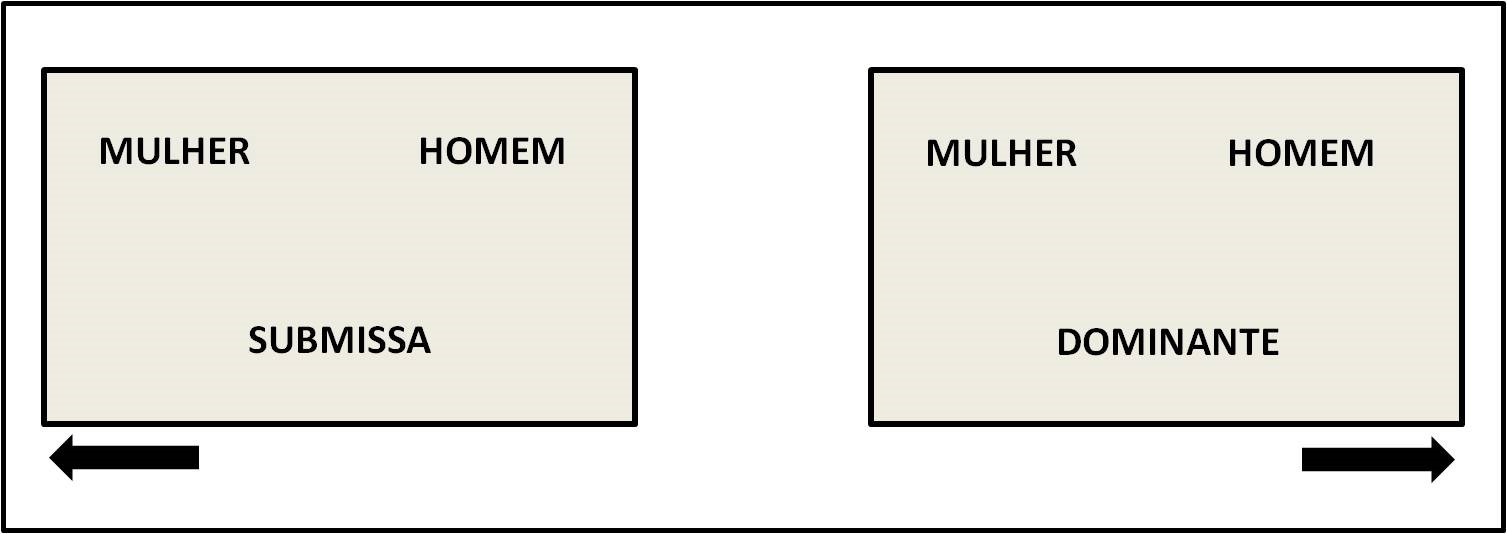
\includegraphics[width=\linewidth]{5/figura1.jpg}
    \caption{Modelo esquemático da apresentação dos estímulos em duas tentativas hipotéticas do IAT. À esquerda, a resposta considerada correta nas tentativas consistentes é apresentada pela seta preta, ou seja, na direção da categoria ``mulher''. À direita, a resposta considerada correta nas tentativas consistentes está na direção da categoria ``homem''.}
    \label{fig1}
\end{figure}

Uma alternativa ao IAT é o IRAP (da sigla em inglês para \textit{Implicit Relational Assessment Procedure} ou Procedimento de Avaliação Relacional Implícita), de Barnes-Holmes et al. (2006), que é um procedimento que utiliza as tarefas experimentais semelhantes às do IAT, porém com uma operacionalização mais aproximada da Análise do Comportamento. O IRAP é baseado em várias teorias comportamentais, como a teoria do comportamento verbal (Skinner, 1957), o paradigma de equivalência de estímulos (Sidman, 1971; 1997), e a Teoria das Molduras Relacionais (Hayes, Barnes-Holmes, \& Roche, 2001). Essas teorias comportamentais sobre o desenvolvimento do comportamento simbólico apresentam a aprendizagem, em contingências sociais, das respostas a relações entre estímulos como determinante de repertórios de responder imediato, implicados nas atitudes implícitas, durante a formação de categorias de estímulos. Assim, uma maior latência das respostas emitidas diante de uma relação entre dois estímulos (por exemplo, mulher-dominante, em comparação com homem-dominante), é interpretada como a dificuldade de modificar a função de estímulos equivalentes, como já demonstrado pela literatura (Barnes, Browne, Smeets, \& Roche, 1995; Barnes \& Keenan, 1993), especialmente quando a nova função que se quer instalar é inconsistente ou incompatível com a função inicial do estímulo no controle das respostas do indivíduo a estímulos equivalentes\footnote{O paradigma de equivalência de estímulos proposto por Sidman (1971) é um modelo experimental da aquisição de comportamento simbólico que tem sido amplamente confirmado por dados experimentais de pesquisas tanto com humanos como com animais não-humanos (p. ex., Sidman, 1994). Sidman (1971) e Sidman e Cresson (1973), ensinaram, a jovens com atraso cognitivo severo, relações entre palavras faladas e desenhos, bem como relações entre palavras faladas e palavras impressas. Posteriormente, verificaram a emergência de relações de equivalência (o responder diante de novas relações nunca apresentadas no procedimento, de forma coerente com as relações aprendidas) entre figuras e palavras impressas, indicando que estas haviam adquirido o status de símbolos para estes participantes. Os estudos na área compreendem, tipicamente, uma fase de ensino de uma linha de base de relações condicionais entre estímulos usando-se o procedimento de MTS, seguida por uma fase de teste de relações emergentes. Os participantes que aprendem as relações ensinadas na linha de base mostram respostas coerentes diante de relações não treinadas, atestando que a função dos estímulos se tornou equivalente no controle do comportamento dos participantes.}. A função inicial do estímulo no controle do comportamento individual é aprendida em contingências sociais, dentro da cultura do indivíduo e ao longo de sua vida, sem necessariamente transferir-se para o controle do relato verbal desse indivíduo sobre seu próprio comportamento. Dentro do modelo de significado proposto pelo paradigma de equivalência de estímulos (p. ex., Sidman, 1971 e Sidman \& Cresson, 1973), as palavras e conceitos podem adquirir a mesma função no controle do comportamento a depender de relações estabelecidas dentro de uma rede, que torna os estímulos equivalentes, mesmo que não necessariamente relacionados diretamente por meio de experiência direta de condicionalidade. Por exemplo, uma pessoa pode – ao longo da sua história de aprendizagem social – nunca ter sido ensinada diretamente que ``mulheres são submissas'', mas, por meio de regras não explicitadas e de aprendizagens em contingências específicas, pode ter aprendido que ``mulheres são fracas'' e também ter aprendido a relação entre os estímulos ``pessoas fracas'' e ``submissão'', e então responder da mesma maneira à relação ``mulheres-submissão'', por transitividade das relações aprendidas anteriormente, que possuem o mesmo significado em determinados contextos do ambiente cultural. O IRAP seria, então, sensível a esse fenômeno, dado que os participantes são instruídos a responder coerentemente a determinadas relações condicionais apresentadas entre estímulos estereotipicamente relacionados dentro da cultura. Quando as relações já foram aprendidas anteriormente, e as classes de estímulos equivalentes já estão presentes no controle do repertório de respostas do indivíduo, espera-se que ele responda de maneira mais rápida durante o procedimento.

No procedimento do IRAP, a tarefa experimental é apresentada ao participante na tela do computador, e em cada tentativa são apresentados dois estímulos e duas opções de resposta (que podem ser ``correto'' e ``incorreto'', ``sim'' e ``não'', ``combina'' ou ``não combina'', etc.). O participante deve responder o mais rápido possível a uma dessas opções, diante da relação entre os dois estímulos na tela. São apresentados blocos de tentativas de treino das relações condicionais entre os estímulos e, em seguida, blocos consecutivos de tentativas de teste das relações treinadas, em que a resposta é considerada correta quando é consistente com aquela hipotetizada pelos experimentadores como produto da aprendizagem social (isto é, as respostas a relações estereotipadas do tipo ``mulher-submissa'' e ``homem-dominante''; ou ``menina-boneca'' e ``menino-carrinho''), ou blocos em que as respostas são consideradas corretas quando são inconsistentes com os estereótipos sociais (por exemplo, diante das relações ``mulher-dominante'' e ``homem-submisso''; ou ``menina-carrinho'' e ``menino-boneca''). Além disso, respostas somente são consideradas corretas se forem emitidas dentro de um período de 2s da apresentação da tentativa, caso contrário, serão consequenciadas e registradas como incorretas. Espera-se, então, que os participantes levem mais tempo para responder corretamente às tentativas de teste dos blocos inconsistentes do que às tentativas dos blocos consistentes. A Figura \ref{fig2} mostra um exemplo hipotético da configuração das tentativas apresentadas durante um procedimento de IRAP. As respostas consideradas corretas, nos blocos de tentativas de treino, são seguidas da próxima tentativa (ou seja, não há consequências específicas para acerto) e as respostas consideradas incorretas, inclusive nas tentativas em que não houve resposta dentro do tempo limite de 3s, são seguidas de consequência negativa (por exemplo, a palavra ``incorreto'' ou um X vermelho na tela do computador) e da reapresentação da mesma tentativa até que o participante emita a resposta designada como correta naquela tentativa. 

\begin{figure}[t]
    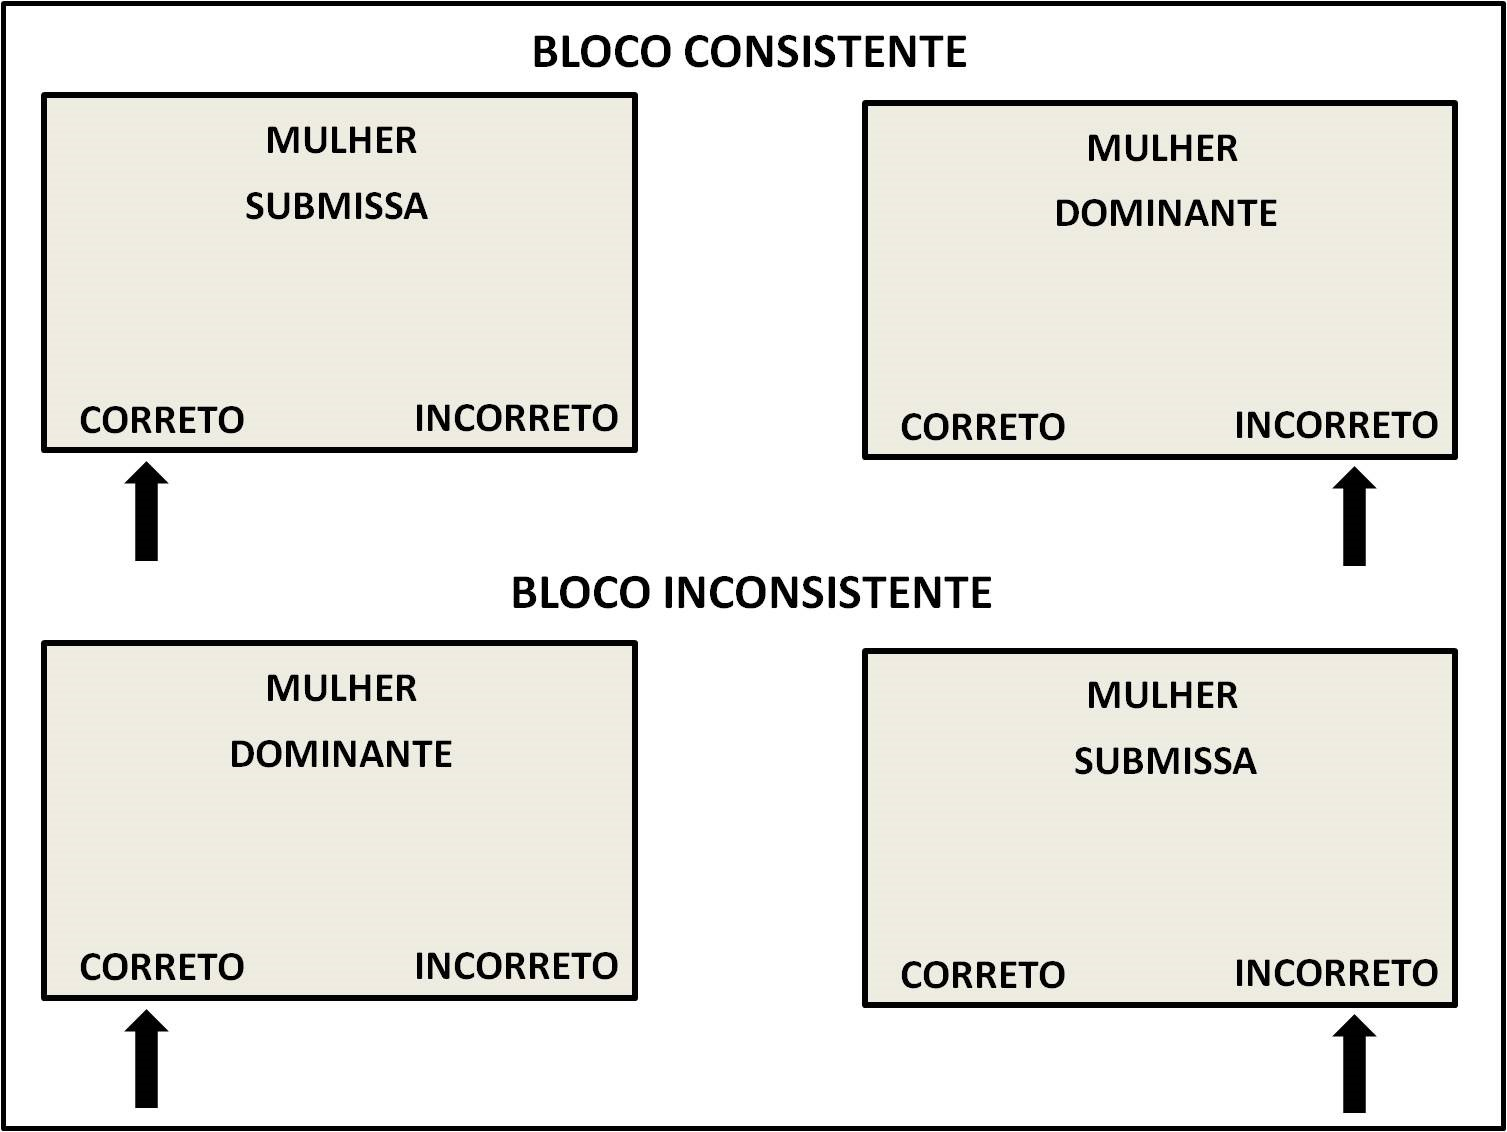
\includegraphics[width=\linewidth]{5/figura2.jpg}
    \caption{Modelo esquemático da apresentação dos estímulos nos quatro tipos de tentativas hipotéticas do IRAP. Nos blocos consistentes (acima) e nos blocos inconsistentes (abaixo) a resposta considerada correta deve ser clicar sobre a palavra que está indicada pela seta preta.}
    \label{fig2}
\end{figure}

Diversas demonstrações experimentais mostram que o IRAP pode ser usado de maneira eficiente para detectar atitudes implícitas em relação a gênero, e que os resultados do IRAP replicam o fenômeno já demonstrado com o IAT, na comparação com instrumentos de medida de atitudes explícitas, de que o relato verbal de atitudes diante de determinados contextos não é preditivo do comportamento atitudinal implícito diante do mesmo contexto. Um levantamento feito por Freitas (2017) encontrou sete estudos que usaram o IRAP para estudar estereótipos e vieses de gênero, e os resultados mostram que esse teste é sensível para detectar essas atitudes em diversos contextos. Drake e cols. (2010) realizaram quatro estudos para avaliar a sensibilidade e a aplicabilidade do IRAP, buscando acrescentar avaliações de viés de raça, religião, gênero e obesidade à literatura experimental referente ao instrumento. No estudo que avaliou atitudes quanto a gênero, foram realizadas duas aplicações consecutivas do IRAP, uma em que os estímulos utilizados foram as palavras ``homem'' e ``mulher'' e profissões estereotipicamente masculinas e femininas, e outra em que os estímulos eram as palavras ``homem'' e ``mulher'' e afazeres domésticos considerados masculinos e femininos. Os resultados mostraram diferença entre as médias dos escores do IRAP para as ocupações estereotipicamente femininas, no grupo de mulheres (mulheres responderam mais rápido a relações estereotipicamente consistentes entre a palavra ``mulher'' e as ocupações femininas do que a relações inconsistentes entre esses estímulos); o mesmo aconteceu no grupo de participantes homens para as relações consistentes entre a palavra ``homem'' e as ocupações masculinas. A diferença nas outras relações não foi significativa. Esse resultado confirma a literatura sobre profissões estereotipicamente femininas, e reforça a hipótese de que o IRAP é sensível a esse tipo específico de atitude implícita no contexto de gênero.

Algumas vezes o responder atitudinal diante de contextos mistos de estímulos culturais pode mostrar viés mais forte para um tipo de estimulação do que para outro, o que nos leva a inferir que determinadas classes de estímulos equivalentes podem interagir ou até mesmo se sobrepor a outras, no controle do comportamento. Nolan, Murphy e Barnes-Holmes (2013) aplicaram o IRAP em 21 estudantes universitários para verificar atitudes em relação à obesidade, analisando se o peso corporal de uma pessoa influenciava na percepção que os participantes tinham quanto à sua inteligência. Os estímulos utilizados foram fotos de homens e mulheres antes e depois der perderem peso e adjetivos que denotam inteligência ou falta dela, por exemplo, estúpido, idiota, bobo, etc. Os resultados encontrados corroboram a hipótese de que as relações entre os estímulos ``pessoa magra'' e inteligência são muito mais automáticas (e, portanto, implícitas) do que as relações entre ``pessoas gordas'' e inteligência. Quando foram feitas análises específicas por gênero do participante, encontrou-se que os homens mostraram atitude mais favorável para a relação inteligência-magreza quando os estímulos eram fotos de homens do que quando eram fotos de mulheres, enquanto as participantes mulheres não mostraram diferenças na latência da resposta diante dos dois tipos de estímulos. Isso pode ser interpretado como uma interferência das atitudes dos participantes homens em relação ao gênero feminino no responder diante das relações entre os estímulos ``mulher'' e palavras denotativas de inteligência.

Estudos têm demonstrado que essas aprendizagens relacionais são adquiridas desde cedo no desenvolvimento dos indivíduos, provavelmente por estarem constantemente, desde antes do nascimento, em contato com as relações sociais e as práticas culturais vigentes em sua comunidade verbal. Além disso, determinados repertórios de responder relacional a configurações de estimulação do ambiente podem levar a maior ou menor grau de atitudes diante de contextos específicos. Scanlon, McEnteggart, Barnes-Holmes e Barnes-Holmes (2014) buscaram avaliar viés implícito de gênero e autoestima em crianças com desenvolvimento típico, crianças com TDAH (Transtorno do Déficit de Atenção com Hiperatividade) e crianças com dislexia. O primeiro estudo teve como participantes crianças de 8 a 11 anos, tanto com TDAH quanto com desenvolvimento típico. Os estímulos utilizados eram o nome da própria criança e um nome do outro gênero, além de três adjetivos positivos e três negativos. Os resultados mostraram que ambos os grupos apresentavam graus diferentes de atitude implícita positiva em relação a si mesmo. As crianças com desenvolvimento típico não mostraram nenhum viés em relação ao nome de outro gênero, mas as crianças com TDAH mostraram atitudes negativas quanto ao nome do gênero oposto ao delas, além das atitudes positivas quanto a si mesmas. Já o segundo estudo teve como participantes 20 crianças de nove a 14 anos, com desenvolvimento típico e com dislexia. O procedimento foi o mesmo que no primeiro estudo. Como resultado, ambos os grupos mostraram viés a favor de si mesmo tanto nos testes do tipo ``eu-positivo'' e ``eu-negativo'', e ambos os grupos não foram nem positivos nem negativos no julgamento da relação ``outro-positivo''. Contudo, as crianças de desenvolvimento típico mostraram viés contrário ao outro nas tentativas do tipo ``outro-negativo'', enquanto as que tinham dislexia mostraram viés a favor. Outro estudo com crianças foi o de Rabelo, Bortoloti e Souza (2014), que envolveu 10 crianças de sete a 10 anos. Os estímulos utilizados foram nomes femininos e masculinos e brinquedos tipicamente designados a cada um dos gêneros (bonecas e carrinhos). As crianças de ambos os sexos responderam significativamente mais rápido nas tentativas que relacionavam que bonecas eram para meninas e que bonecas não eram para meninos. As relações com os carrinhos não foram significativas. 

A história de aprendizagem de práticas culturais vigentes no grupo em que o indivíduo se insere pode ser responsável pelo viés implícito apresentado pelas pessoas ao longo da vida, de maneira inconsciente e muitas vezes difícil de detectar em situações cotidianas\footnote{Para análises mais aprofundadas das implicações dos repertórios atitudinais implícitos, veja os capítulos 02 e 04 deste livro, que fazem discussões acerca das consequências da desigualdade de gêneros.}. Farrell, Cochrane e McHugh (2015) utilizaram o IRAP com 32 adultos (sendo 16 homens e 16 mulheres), usando como estímulos as palavras homem e mulher e nomes de carreiras profissionais. Os resultados mostraram que, de maneira geral, os participantes associaram mais as carreiras de ciência, tecnologia, engenharia e matemática com homens e as carreiras artísticas com mulheres. Esse efeito foi mais proeminente nas participantes mulheres; os homens tenderam a responder de maneira mais neutra. Já Hussey e cols. (2016) investigaram o fenômeno da desumanização\footnote{O fenômeno da desumanização acontece quando emitimos comportamentos que denotam que pessoas do gênero feminino têm o mesmo valor ou função que objetos. Esse tipo de repertório está implicado, por exemplo, no uso da imagem de mulheres consideradas sexualmente atrativas para vender produtos, como é feito em propagandas de cerveja.} das mulheres, também usando o IRAP. Participaram da pesquisa 43 homens heterossexuais, com média de idade de 20 anos, que responderam o IRAP, buscando investigar até que ponto os vieses de resposta em relação às mulheres eram influenciados por duas categorias diferentes de contraste: ``homens'' e ``objetos inanimados''. Os resultados indicaram que a maior desumanização das mulheres foi observada no contexto deste último em relação à primeira categoria, ou seja, os participantes tenderam a responder mais rápido às relações que implicavam que mulheres eram diferentes de humanos do que às relações entre estímulos que denotavam que mulheres são iguais a humanos, nas tentativas em que a comparação era com objetos inanimados. Os autores do texto destacaram que o IRAP pode ser descrito como uma medida não relativa, mas não sem contexto, de respostas relacionais breves e imediatas\footnote{Respostas Relacionais Breves e Imediatas (BIRR) se contrapõem a Respostas Relacionais Elaboradas e Estendidas (EERR). As primeiras estariam relacionadas a tarefas de atitude implícita, nas quais a resposta do participante tem que ser emitida em um curto espaço de tempo. As últimas estariam relacionadas a tarefas de atitude explícitas, nas quais o participante tem tempo de elaborar uma resposta.}. 

Os repertórios individuais de responder atitudinal em relação ao gênero feminino, aprendidos dentro da cultura, têm implicação direta em práticas que mantêm e replicam desigualdade entre os gêneros, como aquelas que levam ao fenômeno do \textit{gender gap}, ou a diferença de acesso à riqueza advinda da menor remuneração recebida pelas mulheres (ONU, 2015, \textit{Minimum Set of Gender Indicators}). É comum que, dentro dessas práticas, possamos observar a existência de um binarismo marcado pelo responder atitudinal positivo diante de estímulos e características estereotipicamente consideradas masculinas em detrimento da atitude positiva em relação a estímulos e características estereotipicamente consideradas femininas, e que essa é uma propriedade intrínseca das relações entre os estímulos do contexto de gênero. Ou seja, as características consideradas masculinas têm valores positivo e as características femininas têm valores negativos, em contraposição umas às outras, formando pares opostos, como na afirmação ``mulheres são submissas e homens são dominantes''. Cartwright, Hussey, Roche, Dunne e Muphy (2017) usaram o IRAP com 47 estudantes universitários, e compararam os resultados de atitude implícita diante dos gêneros com uma medida de autorrelato sobre estereótipos de gênero e também com uma tarefa de simulação de contratação para emprego. Para o IRAP, os estímulos utilizados foram as palavras ''homem'' e ''mulher'' e características estereotipicamente femininas e masculinas, tanto positivas quanto negativas, escolhidas entre aquelas consideradas pelos participantes como altamente desejáveis e altamente indesejáveis, entre um conjunto de características humanas. Os efeitos encontrados no IRAP estavam na direção esperada (os participantes responderam de acordo com as relações de estereótipos aprendidas socialmente). No entanto, os resultados mostraram que as características masculinas foram consideradas como mais desejáveis pela maioria dos participantes (83\%), mostrando que 1) traços de gênero parecem ser enquadrados de forma oposta na linguagem; e 2) este binarismo pode sustentar hierarquias de gênero existentes em certos contextos. Drake, Primeaux e Thomas (2018) também usaram o IRAP e investigaram estereótipos de gênero com 50 participantes adultos. O resultado corroborou aqueles já encontrados na literatura: homens e mulheres relacionaram mais rapidamente os gêneros com certas características estereotípicas contrastantes (sensível e emocional para mulheres, dominante e lógico para homens). Nesse estudo, os resultados mostrados pelo IRAP foram replicados para os participantes também com o IAT.

O IRAP tem sido usado amplamente em experimentos sobre atitudes implícitas para demonstrar empiricamente a função de relações de estímulos aprendidas em contexto social no controle do comportamento atitudinal, tanto com participantes adultos como com crianças. Embora os resultados sejam expressivos e repliquem as literaturas tanto da área de atitudes implícitas quanto de sociologia e antropologia no que diz respeito a estereótipos de gênero, discriminação e viés de gênero, o IRAP é um procedimento longo e que depende de treino extensivo dos participantes, necessitando muitas vezes de mais de uma sessão experimental para sua realização, o que pode resultar em perdas de participantes ao longo dos estudos e em uma necessidade de tempo disponível maior para o engajamento do participante na pesquisa. Já o \textit{Funcional Acquisition Speed Test} (FAST, da sigla em inglês para Teste de Rapidez de Aquisição de Função) também é um teste de medida implícita (O'Reilly, Roche, Ruiz, Tyndall, \& Gavin, 2012), que é defendido por seus autores como mais consistente com os princípios analítico-comportamentais no estudo de atitudes implícitas, quando comparado ao IAT e o IRAP. Segundo os autores, quatro argumentos podem ser colocados para defender o uso do FAST: 1) tradicionalmente, na Análise Experimental do Comportamento, não usamos o tempo de reação (latência da resposta) como medida de força ou estabilidade de comportamentos, e sim como demonstração de acurácia e fluência do responder; 2) o IRAP apenas provê consequências quando o participante responde em desacordo com o estabelecido pelo teste como resposta correta, o que seria um esquema de punição, que não é o que a Análise do Comportamento considera como o procedimento eficaz para gerar fluência; 3) o IRAP utiliza técnicas estatísticas de manipulação dos dados brutos para gerar o resultado final de escores de latência padronizados, enquanto o FAST usa medidas diretas da taxa de aprendizagem, dada pela frequência de respostas consideradas corretas ao longo das tentativas apresentadas (que podem ser analisadas tanto individualmente quanto em medidas de grupo); e 4) para aumentar a significância estatística, o IRAP usa estratégias de valor-limite dos dados e eliminação de participantes cujos dados estão fora da distribuição esperada para o instrumento, que são métodos típicos da área de psicometria, tradicionalmente rejeitados e criticados por pesquisadores de Análise do Comportamento (p. ex., Skinner, 1953 e Sidman, 1960). Além disso, o FAST tem se mostrado um procedimento mais simples, mais rápido (a aplicação leva em torno de 15 minutos) e mais fácil de ser analisado, pois não demanda tratamento dos dados anterior às análises estatísticas de significância e correlação, precisando-se apenas calcular a inclinação das curvas de aprendizagem nos blocos consistente e inconsistente.

No FAST, ao invés de treinar os participantes para responder com acurácia e rapidez a uma tarefa de categorização e depois comparar a latência das respostas nos blocos de teste consistente e inconsistente, usa-se como medida a diferença na \textit{velocidade de aquisição} de uma função em comum para cada categoria. Durante o procedimento do FAST, estímulos com a mesma função no controle do comportamento devem ser seguidos da mesma resposta, e estímulos com outra função devem ser seguidos de outra resposta, configurando duas classes funcionais de estímulos distintas. Os participantes são expostos a um bloco de tentativas de treino da tarefa, usando-se conjuntos de estímulos familiares (por exemplo, as palavras ``gato'' e ``cachorro'' devem controlar a respostas de pressionar a tecla M do teclado do computador e as palavras ``camisa'' e ``calça'' devem controlar a resposta de pressionar a tecla Z). Depois do bloco de treino da tarefa, o participante é exposto a dois blocos de tentativas do FAST propriamente dito: um bloco de tentativas consistentes com estímulos relacionados na aprendizagem cultural (o participante deve apertar a tecla Z para ``mulher'' e para palavras como ``sensível'' e a tecla M para ``homem'' e palavras como ``dominante'', por exemplo), e blocos inconsistentes com essas aprendizagens estereotípicas (apertar a tecla Z para ``mulher'' e ``dominante'' e a tecla M para ``homem'' e ``sensível''). Nas tentativas do FAST, apenas um estímulo é apresentado na tela do computador e o participante tem um tempo limite de 3s para emitir a resposta, caso contrário ela será consequenciada e registrada como incorreta. O procedimento do FAST pode ser considerado como um procedimento de ensino de discriminações simples, enquanto os procedimentos do IAT e do IRAP são procedimentos que requerem aprendizagem de relações de discriminação condicional entre os estímulos. No FAST tanto respostas consideradas corretas como respostas consideradas incorretas em cada tipo de bloco são seguidas de consequências (por exemplo, das palavras ``correto'' e ``incorreto'', respectivamente) ao longo de todo procedimento, e não há blocos de teste (blocos sem consequências para medir a quantidade de respostas corretas depois do treino, como no IRAP), já que a medida da variável dependente é a aquisição das respostas funcionalmente distintas em cada bloco. Os dados são registrados e uma curva de respostas acumuladas (Skinner, 1961) é construída, sendo a inclinação da curva a medida da velocidade de aprendizagem. A Figura \ref{fig3} apresenta um conjunto de tentativas hipotéticas do FAST para um estudo sobre atitudes machistas.

\begin{figure}[t]
    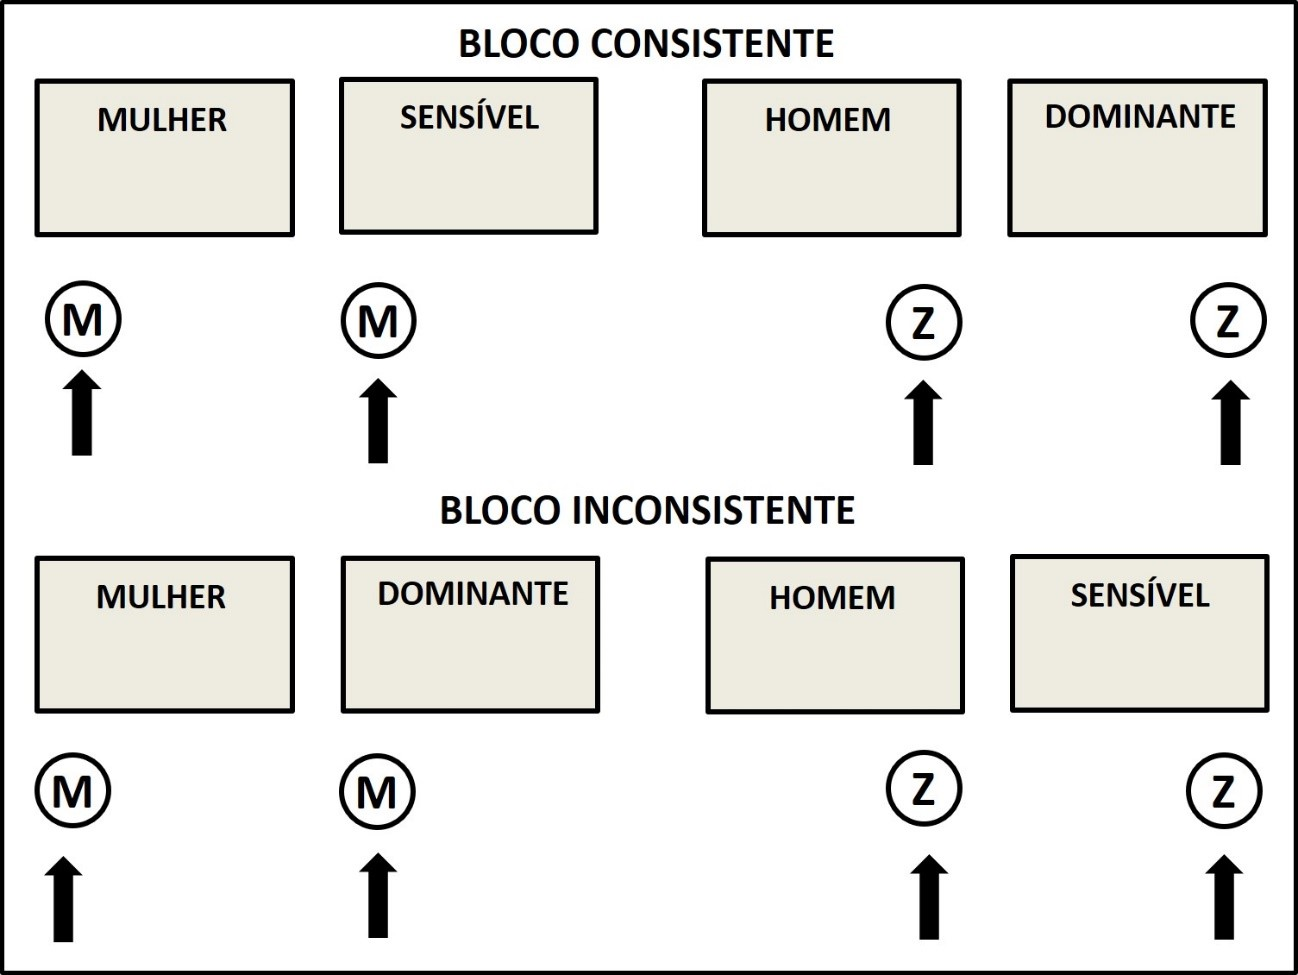
\includegraphics[width=\linewidth]{5/figura3.jpg}
    \caption{Modelo esquemático dos quatro tipos de tentativas hipotéticas do FAST para cada um dos blocos (consistente e inconsistente). Nos blocos de tentativas consistentes (acima) e nos blocos de tentativas inconsistentes (abaixo), a resposta considerada correta é pressionar a mesma tecla do computador, indicada pela seta preta, para cada uma das categorias consideradas corretas naquele bloco.}
    \label{fig3}
\end{figure}

Para verificar a validade do FAST na detecção de relações estereotípicas entre estímulos aprendidas em contexto social, O'Reilly e cols. (2012) fizeram um estudo, com 23 participantes, em que relações condicionais entre estímulos abstratos foram ensinadas em ambiente experimental e depois testaram se o FAST seria eficiente em demonstrar a força das relações entre os estímulos relacionados. Em uma das fases experimentais, os participantes eram submetidos a um procedimento de MTS em que aprendiam a relacionar dois pares de estímulos: A1-B1 e A2-B2. As outras três fases eram pares de blocos de tentativas consistentes e inconsistentes com as relações aprendidas usando o procedimento FAST, tanto com os estímulos treinados na fase de MTS quanto com novos estímulos para estabelecer uma linha de base de comparação. Os resultados mostraram que dos 18 participantes que terminaram o estudo, 13 fizeram 10 acertos consecutivos mais rapidamente no bloco consistente que no bloco inconsistente usando as relações treinadas anteriormente, mostrando que o FAST pode ser usado para determinar a existência prévia de relações entre estímulos. Posteriormente, outro estudo (O'Reilly, Roche, Gavin, \& Ruiz, 2013) testou se o FAST era capaz de medir a existência e a força de relações derivadas daquelas ensinadas em laboratório usando o paradigma de equivalência de estímulos (Sidman, 1971). Esse teste é especialmente importante, pois, como os autores apontam, as relações verbais aprendidas nas contingências sociais da comunidade verbal muitas vezes estão em cadeias complexas dentro de classes de estímulos equivalentes. Nesse estudo, 24 participantes passaram por três fases experimentais. Na fase 1, receberam treino de relações condicionais com o procedimento de MTS para estabelecer as relações AB e AC. Na fase 2, foram testadas as relações emergentes que atestam a formação de classes de estímulos equivalentes. A fase 3 consistiu em uma série de apresentações do FAST: usando tanto estímulos relacionados diretamente durante o treino de relações condicionais com o procedimento de MTS, como estímulos cujas relações entre si eram emergentes dentro das classes de estímulos equivalentes formadas. Os resultados mostraram que o FAST é sensível para detectar tanto as relações diretamente treinadas quanto as relações derivadas entre os estímulos das classes de equivalência.

As demonstrações experimentais das variáveis envolvidas no procedimento de FAST com relações estabelecidas em laboratório atestam que este é um procedimento válido e eficiente para medidas de atitudes implícitas consistente com a Análise do Comportamento. Sendo assim, pesquisas aplicadas sobre atitudes explícitas do tipo viés de gênero, preconceito e machismo podem se beneficiar do uso do FAST como medida da força das relações aprendidas socialmente dentro de uma cultura. Por exemplo, um estudo recente (Cartwright, Roche, Gogarty, O'Reilly, \& Stewart, 2016) avaliou, pela primeira vez, a sensibilidade do FAST a relações naturais (não treinadas em laboratório), ao verificar estereótipos de gênero implícitos dos participantes quanto a características estereotipicamente femininas e masculinas. Para isso, os experimentadores selecionaram palavras consideradas tradicionalmente como qualidades masculinas (``dominante'', ``racional'', ``competitivo'' e ``agressivo'') e femininas (``submissa'', ``emocional'', ``cooperativa'' e ``passiva'') e formaram duas categorias consistentes entre um estímulo rótulo (a palavra ``homem'' ou a palavra ``mulher'') e os estímulos de características consideradas masculinas na categoria ``homem'' e os estímulos de características femininas na categoria ``mulher''. Os blocos de tentativas inconsistentes apresentavam os estímulos ``homem'' e características consideradas femininas controlando a mesma resposta e os estímulos ``mulher'' e características masculinas controlando outra resposta. Trinta estudantes universitários foram participantes do estudo. Além dos blocos de FAST, eles também foram submetidos à apresentação do IAT e a dois questionários de autorrelato para a medida da atitude explícita. Os resultados mostraram que o FAST é sensível a relações verbais anteriormente aprendidas entre estímulos – mais especificamente a relações pervasivas de estereótipo de gênero. Todos os 30 participantes mostraram efeitos na direção esperada: aprendizagem mais rápida da resposta comum no bloco de tentativas consistentes do que no bloco de tentativas inconsistentes. Além disso, para os 27 dos 28 participantes que concluíram também o IAT, os resultados mostraram latências mais curtas nas respostas dos blocos de relações consistentes com os estereótipos de gênero. Como esperado pelos pesquisadores, não foram encontradas correlações entre as medidas implícitas e explícitas.

A importância de se ter um teste de medida implícita para se estudar estereótipo de gênero é mais bem compreendida quando pensamos que a desigualdade de gênero é um problema social a nível global, preocupando diversos países no mundo e mobilizando instituições e governos a superá-lo, sendo inclusive uma das metas da Organização das Nações Unidas (ONU, 2015). No Brasil, o Centro de Atendimento à Mulher, que tem um plantão telefônico (180), indicou que entre 2014 e 2015 houve aumento na denúncia de crimes contra mulheres: de 300,39\% nas denúncias de cárcere privado, de 165,27\% nos casos de estupro e de 161,42\% nos relatos de tráfico de pessoas.

Esses dados mostram que o gênero é uma variável relevante na interação verbal entre pessoas. Ruiz (2003) destaca que o gênero é uma fonte tênue de controle de estímulos no comportamento das pessoas, mas que gera contingências muito diferentes para homens e mulheres dentro da sociedade. Nesse estudo, Ruiz (2003) cita diversos exemplos (e.g., Sadker \& Sadker, 1994; Irvine, 1986) de como professores tratam diferentemente meninos e meninas na escola, dando significantemente mais atenção para eles nas aulas e elogiando-os por suas ideias e trabalho enquanto elogiam as meninas pela aparência de seus trabalhos e por elas seguirem regras.

Os estudos experimentais e os diversos procedimentos usados na área de atitudes implícitas demonstram que o aprendizado das relações simbólicas e arbitrárias entre estímulos de naturezas diferentes presentes no ambiente físico ou verbal de um indivíduo, ao longo de sua história dentro de uma cultura, leva a repertórios de comportamentos que se expressam não somente no nível verbal, mas em respostas que agem diretamente sobre o meio físico ou social. As redes de relações entre estímulos estabelecidas pelas práticas culturais tornam virtualmente impossível que analisemos os fenômenos comportamentais humanos sem uma compreensão ampla dos contextos em que essas relações foram aprendidas e quais as funções que elas adquirem no controle do comportamento dos indivíduos dentro do grupo. Para de Rose (2016) 

\begin{quote}
    Isto inclui uma ampla gama de funções, que podem ser agrupadas em discriminativas, eliciadoras e reforçadoras condicionadas. Assim, se um estímulo é discriminativo, eliciador, ou reforçador condicionado, estímulos coordenados a ele podem adquirir estas mesmas funções, mesmo que não tenha havido para eles um treino específico de discriminação operante ou de condicionamento respondente (p. 210).
\end{quote}

Na prática, isso quer dizer que, numa situação social, quando rimos de comentários machistas sobre a roupa de uma mulher, estamos reforçando as relações entre esses estímulos, relações que participam de uma rede complexa de relações com outros estímulos, respostas e reforçadores, que também terão suas probabilidades de ocorrência modificadas. Atitudes implícitas são o produto do controle simbólico sobre o comportamento das pessoas dentro de uma cultura. Para além da descrição das relações entre eventos que controlam as respostas atitudinais implícitas, o uso de procedimentos experimentais que evidenciam a força dessas relações no controle dos comportamentos verbais e não verbais dos indivíduos dentro de uma prática cultural é necessário para que a Análise do Comportamento passe a considerar esses contextos de controle como parte imprescindível em uma análise cultural que se traduza em mudança efetiva de sistemas de opressão.
\vfill
\pagebreak
\section*{Referências Bibliográficas}\sectionmark{Referências Bibliográficas}

\hangindent=25pt
\hangafter=1
\noindent Ajzen, I., \& Madden, T.J. (1986). Prediction of goal-directed behavior-attitudes, intentions, and perceived behavioral-control. Journal of Experimental Social Psychology, 22(5), 453-474.

\hangindent=25pt
\hangafter=1
\noindent Barnes, D., \& Keenan, M. (1993). A transfer of functions through derived arbitrary and nonarbitrary stimulus relations. Journal of the Experimental Analysis of Behavior, 59(1), 61-81.

\hangindent=25pt
\hangafter=1
\noindent Barnes, D., Browne, M., Smeets, P., \& Roche, B. (1995). A transfer of functions and a conditional transfer of functions through equivalence relations in three-to six-year-old children. The Psychological Record, 45(3), 405-430.

\hangindent=25pt
\hangafter=1
\noindent Barnes-Holmes, D., Barnes-Holmes, Y., Power, P., Hayden, E., Milne, R., \& Stewart, I. (2006). Do you really know what you believe? Developing the Implicit Relational Assessment Procedure (IRAP) as a direct measure of implicit beliefs. The Irish Psychologist, 32(7), 169-177.

\hangindent=25pt
\hangafter=1
\noindent Barnes-Holmes, D., Barnes-Holmes, Y., Stewart, I., \& Boles, S. (2010). A sketch of the Implicit Relational Assessment Procedure (IRAP) and the relational elaboration and coherence (REC) model. The Psychological Record, 60, 527-542.

\hangindent=25pt
\hangafter=1
\noindent Bem, D.J. (1965). An experimental analysis of self-persuasion. Journal of Experimental Social Psychology, 1, 199-218.

\hangindent=25pt
\hangafter=1
\noindent Cartwright, A., Roche, B., Gogarty, M., O'Reilly, A., \& Stewart, I. (2016). Using a modified Function Aquisition Speed Test (FAST) for assessing implicit gender stereotypes. The Psychological Record, 66, 223-233.

\hangindent=25pt
\hangafter=1
\noindent Cartwright, A., Hussey, I., Roche, B., Dunne, J., \& Murphy, C. (2017). An investigation into the relationship between the gender binary and occupational discrimination using the Implicit Relational Assessment Procedure. The Psychological Record, 67(1), 121-130.

\hangindent=25pt
\hangafter=1
\noindent Catania, C.A. (2017). Prejudice as verbally governed discrimination. The ABCs of Behavior Analysis: Introduction to Behavior and and Learning, (pp. 254-263). Cornwall-on-Hudson, NY: Sloan Publishing. 

\hangindent=25pt
\hangafter=1
\noindent Crowne, D.P., \& Marlowe, D. (1960). A new scale of social desirability independent of psychopathology. Journal of Consulting Psychology, 24(4), 349-354.

\hangindent=25pt
\hangafter=1
\noindent de Rose, J.C. (2016). A importância dos respondentes e das relações simbólicas para uma Análise Comportamental da Cultura. Acta Comportamentalia, 24(2), 201-220.

\hangindent=25pt
\hangafter=1
\noindent Drake, C.E., Kellum, K.K., Wilson, K.G., Luoma, J.B., Weinstein, J.H., \& Adams, C.H. (2010). Examining the Implicit Relational Assessment Procedure: Four preliminary studies. The Psychological Record, 60(1), 81–100.

\hangindent=25pt
\hangafter=1
\noindent Drake, C.E., Primeaux, S., \& Thomas, J. (2018). Comparing implicit gender stereotypes between women and men with the Implicit Relational Assessment Procedure. Gender Issues, 35(1), 3-20.

\hangindent=25pt
\hangafter=1
\noindent Farrell, L., Cochrane, A., \& McHugh, L. (2015). Exploring attitudes towards gender and science: The advantages of an IRAP approach versus the IAT. Journal of Contextual Behavioral Science, 4, 121-128.

\hangindent=25pt
\hangafter=1
\noindent Fazio, R.H., \& Olson, M.A. (2003). Implicit measures in social cognition research: Their meaning and use. Annual Review of Psychology, 54(1), 297-327.

\hangindent=25pt
\hangafter=1
\noindent Field, D.P., \& Hineline, P.N. (2008). Dispositioning and the obscured roles of time in psychological explanations. Behavior and Philosophy, 36, 5-69.

\hangindent=25pt
\hangafter=1
\noindent Freitas, J.C. (2017). O IRAP como instrumento para identificação de vieses de gênero: uma revisão de literatura. Apresentação Oral em Sessão Coordenada no XXVI Encontro Brasileiro de Psicologia e Medicina Comportamental. Bauru, SP, 7 a 10 de setembro de 2017.

\hangindent=25pt
\hangafter=1
\noindent Gawronski, B., \& Bodenhausen, G.V. (2006). Associative and propositional processesin evaluation: an integrative review of implicit and explicit attitude change. Psychological Bulletin, 132(5), 692-731.

\hangindent=25pt
\hangafter=1
\noindent Greenwald, A.G., McGhee, D.E., \& Schwartz, J.L. (1998). Measuring individual differences in implicit cognition: The Implicit Association Test. Journal of Personality and Social Psychology, 74, 1464-1480.

\hangindent=25pt
\hangafter=1
\noindent Guerin, B. (1994). Attitudes and beliefs as verbal behavior. The Behavior Analyst, 17(1), 155-163.

\hangindent=25pt
\hangafter=1
\noindent Hayes, S.C., Barnes-Holmes, D., \& Roche, B. (Eds.). (2001). Relational Frame Theory: A post Skinnerian account of human language and cognition. New York: Plenum Press.

\hangindent=25pt
\hangafter=1
\noindent Hineline, P.N. (1990). The origins of environment-based psychological theory. Journal of the Experimental Analysis of Behavior, 53(2), 305-320.

\hangindent=25pt
\hangafter=1
\noindent Holland, J. (1973). ¿Servirán los principios conductuales para los revolucionarios? Em F.S. Keller \& E.R. Iñesta, (Orgs.), Modificación de la conduta: Aplicaciones a la educación. México: Trillas.

\hangindent=25pt
\hangafter=1
\noindent Hussey, I., Mhaoileoin, D.N., Barnes-Holmes, D., Ohtsuki, T., Kishita, N., Hughes, S., \& Murphy, C. (2016). The IRAP is nonrelative but not acontextual: Changes to the contrast category influence men’s dehumanization of women. The Psychological Record, 66(2), 291-299. 

\hangindent=25pt
\hangafter=1
\noindent Israel, A.C. (1978). Some thoughts on correspondence between saying and doing. Journal of Applied Behavior Analysis, 11(2), 271-276.

\hangindent=25pt
\hangafter=1
\noindent Israel, A.C., \& O'Leary, K.D. (1973). Developing correspondence between children's words and deeds. Child Development, 14, 575-581.

\hangindent=25pt
\hangafter=1
\noindent Kashima, Y., Gallois, C., \& McCamish, M. (1993). The theory of reasoned action and cooperative behaviour: It takes two to use a condom. British Journal of Social Psychology, 32, 227-239.

\hangindent=25pt
\hangafter=1
\noindent Lloyd, K.E. (1994). Do as I say, not as I do. The Behavior Analyst, 17(1), 131-139.

\hangindent=25pt
\hangafter=1
\noindent Maio, G.R., Haddock, G., Manstead, A.S., \& Spears, R. (2010). Attitudes and intergroup relations. Em T.D. Nelson, (Ed.), Handbook of prejudice, stereotyping, and discrimination, (pp. 261-275). New York: Psychology Press. 

\hangindent=25pt
\hangafter=1
\noindent Nolan, J., Murphy, C., \& Barnes-Holmes, D. (2013). Implicit relational assessment procedure and body-weight bias: Influence of gender of participants and targets. The Psychological Record, 63(3), 467-488.

\hangindent=25pt
\hangafter=1
\noindent Nosek, B.A., Hawkins, C.B., \& Frazier, R.S. (2011). Implicit social cognition: from measures to mechanisms. Trends in Cognitive Sciences, 15, 152-159.

\hangindent=25pt
\hangafter=1
\noindent O'Reilly, A., Roche, B., Gavin, A., \& Ruiz, M. R. (2013). A function acquisition speed test for equivalence relations (FASTER). The Psychological Record, 63, 707-724.

\hangindent=25pt
\hangafter=1
\noindent O'Reilly, A., Roche, B., Ruiz, M., Tyndall, I., \& Gavin, A. (2012). The function acquisition speed test (FAST): a behavior analytic implicit test for assessing stimulus relations. The Psychological Record, 62(3), 507–528.

\hangindent=25pt
\hangafter=1
\noindent Organização das Nações Unidas. (2015). Minimum Set of Gender Indicators. Disponível em: https://genderstats.un.org. Última consulta em 13 de abril de 2018.

\hangindent=25pt
\hangafter=1
\noindent Rabelo, L.Z., Bortoloti, R., \& Souza, D.H. (2014). Dolls are for girls and not for boys: Evaluating the appropriateness of the Implicit Relational Assessment Procedure for school-age children. The Psychological Record, 64(1), 71-77.

\hangindent=25pt
\hangafter=1
\noindent Ruiz, M. R. (2003). Inconspicuous sources of behavioral control: The case of gendered practices. The Behavior Analyst Today, 4(1), 12-16. \url{http://dx.doi.org/10.1037/h0100005}

\hangindent=25pt
\hangafter=1
\noindent Scanlon, G., McEnteggart, C., Barnes-Holmes, Y., \& Barnes-Holmes, D. (2014). Using the implicit relational assessment procedure (IRAP) to assess implicit gender bias and self-esteem in typically-developing children and children with ADHD and with dyslexia. Behavioral Development Bulletin, 19(2), 48-59.

\hangindent=25pt
\hangafter=1
\noindent Sidman, M. (1960) Tactics of scientific research. New York: Basic Books.

\hangindent=25pt
\hangafter=1
\noindent Sidman, M. (1971). Reading and auditory-visual equivalences. Journal of Speech and Hearing Research, 14, 5-13.

\hangindent=25pt
\hangafter=1
\noindent Sidman, M. (1994). Equivalence relations and behavior: A research story. Boston: Authors Cooperative.

\hangindent=25pt
\hangafter=1
\noindent Sidman, M. (1997). Equivalence relations. Journal of the Experimental Analysis of Behavior, 68(2), 258-266.

\hangindent=25pt
\hangafter=1
\noindent Sidman, M., \& Cresson, O. (1973). Reading and crossmodal transfer of stimulus equivalences in severe retardation. American Journal of Mental Retardation, 77, 515-523.

\hangindent=25pt
\hangafter=1
\noindent Sidman, M., \& Tailby, W. (1982). Conditional discrimination vs. matching to sample: An expansion of the testing paradigm. Journal of the Experimental Analysis of Behavior, 37, 5-22.

\hangindent=25pt
\hangafter=1
\noindent Sidman, M., Rauzin, R., Lazar, R., Cunningham, S., Tailby, W., \& Carrigan, P. (1982). A search for symmetry in the conditional discrimination of rhesus monkeys, baboons, and children. Journal of the Experimental Analysis of Behavior, 37, 23-44.

\hangindent=25pt
\hangafter=1
\noindent Skinner, B.F. (1961). Why we need teaching machines. Harvard Educational Review, 31, 377-398. 

\hangindent=25pt
\hangafter=1
\noindent Skinner, B. F. (1957). Verbal Behavior. Acton, Massachusetts: Copley.

\hangindent=25pt
\hangafter=1
\noindent Skinner, B. F. (1953) Science and human behavior. New York: Macmillan. 

\hangindent=25pt
\hangafter=1
\noindent Watt, A., Keenan, M., Barnes, D., \& Cairns, E. (1991). Social categorization and stimulus equivalence. The Psychological Record, 41, 33-50.
\chapter{Capítulo}\sectionmark{Seção}
\begin{flushright}
\begin{scriptsize}
Texto
\end{scriptsize}
\vspace{1cm}s

\emph{Citação inicial}
\end{flushright}
\chapter{Capítulo}\sectionmark{Seção}
\begin{flushright}
\begin{scriptsize}
Texto
\end{scriptsize}
\vspace{1cm}s

\emph{Citação inicial}
\end{flushright}
\chapter{Mulheres e tecnologia: aspectos culturais e intervenções comportamentais para aumento da participação feminina na computação}\sectionmark{Mulheres e tecnologia: aspectos culturais e intervenções comportamentais para aumento da participação feminina na computação}\blfootnote{A autora agradece e dedica este capítulo às mulheres responsáveis pelas iniciativas Pyladies São Paulo; Techladies Curitiba e Women Up Games, que além de inspirarem muito do conteúdo aqui apresentado, guiaram e apoiaram seus primeiros passos no mundo da programação.}
\begin{flushright}
\begin{scriptsize}
    Izadora Ribeiro Perkoski  
\end{scriptsize}
\vspace{1cm}
\end{flushright}

O desenvolvimento tecnológico é, assim como a ciência, produto do comportamento humano. Por isso, tanto o processo de desenvolvimento tecnológico quanto seus resultados estão embebidos em valores culturais. O caminho tecnológico que o conhecimento segue é determinado pelo contexto cultural, tanto quanto a inovação é produto da história de reforçamento do inventor. Para Lattal (2003), a tecnologia e a ciência estão intrinsecamente ligados, e o autor define a tecnologia como “a aplicação dos achados científicos a problemas da vida diária” (p. 943), uma definição bastante ampla que abrange a criação de novas ferramentas, métodos, processos e procedimentos para intervir na realidade humana e, evidentemente, abarca muito da produção em Análise do Comportamento. Há algumas características especialmente importantes da tecnologia, segundo Lattal: o fato de que ela não apenas se alimenta da pesquisa científica, mas também retroage sobre a forma como a ciência acontece e, assim como tem o poder de modificar a ciência, a tecnologia também modifica a si mesma – e exemplifica citando a evolução dos computadores.

A Computação é parte da vida diária das pessoas no século XXI, e aos poucos vem sendo adotada e incorporada à Ciência do Comportamento por seu potencial para permitir uma investigação mais refinada e precisa do nosso objeto de estudo. Analistas do comportamento começam a se dedicar a essa intersecção, e a publicação do livro “Introdução ao desenvolvimento de \textit{softwares} para analistas do comportamento” (Neves Filho, de Freitas, \& Quinta, 2018) representa um marco nesse movimento. Um dos capítulos apresenta um manifesto pelo ensino de programação nos cursos de Psicologia e, ao pontuar os desafios relacionados a essa mudança na formação do psicólogo, ressalta:

\begin{quote}
    Outra dificuldade para o ensino de programação nos cursos de Psicologia tem um forte aspecto cultural e tem sido amplamente debatido. As áreas de tecnologia continuam a serem dominadas por homens (este livro infelizmente não foge à regra, por exemplo). Logicamente, a ausência de mulheres nessas áreas ocorre pela falta de estímulo nos períodos escolares. A Psicologia (no Brasil, um curso caracterizado pela grande presença feminina) poderá ajudar a combater este viés ao incluir programação em sua grade curricular, pois estimulará que mulheres aprendam uma habilidade tecnológica e, desse modo, possam exercer melhor papéis de liderança e inovação. (Cardoso, Neves Filho, \& de Freitas, 2018, pp. 169-170).
\end{quote}

Como podemos observar, a baixa participação feminina na Computação se apresenta como um problema com implicações diretas para o desenvolvimento tecnológico da Análise do Comportamento, ciência feita majoritariamente por mulheres. 

Para abordar esse problema, este capítulo adota uma perspectiva feminista. Tal perspectiva pode parecer contraditória, já que muitas vezes o feminismo é pintado como tecnofóbico ou como avesso ao método científico de forma geral (Rothschild, 1981). Apesar disso, há diversas teóricas feministas que se debruçaram sobre o tema da tecnologia e suas intersecções com questões de gênero, tanto na segunda quanto na terceira onda do movimento feminista. A feminista Joan Rothschild (1981), por exemplo, sugere que uma perspectiva feminista da tecnologia pode contribuir tanto para explicitar os valores sexistas que guiam nosso desenvolvimento tecnológico quanto para redirecionar esse desenvolvimento para um caminho mais humanista. 

Portanto, este capítulo tem como objetivo oferecer uma interpretação de base feminista e behaviorista radical para o fenômeno da participação feminina no desenvolvimento tecnológico, mais precisamente na Computação, e oferecer possíveis caminhos de intervenção para modificar esse panorama. 

\section{História das Mulheres na Tecnologia}

O apagamento das mulheres na história\footnote{A história aqui contada é incompleta, limitada e centrada na experiência das mulheres estadunidenses – porque assim são os registros disponíveis. A autora ressalta que a indisponibilidade de informações acerca das mulheres latino-americanas, africanas e asiáticas que certamente tiveram grandes contribuições em seus respectivos países de origem é parte do apagamento exposto, sendo evidência adicional dos problemas aqui relatados.} da produção cultural e tecnológica humana é uma realidade generalizada, seja nas artes, nas ciências ou na história das invenções. Nomes como Margaret Hamilton, Ada Lovelace e Carol Shaw são lembradas como felizes exceções de uma história dominada por homens. Essa é uma forma dramática, talvez inspiradora, talvez revoltante, de contar a história – mas é incompleta. Durante toda a história da Computação, desde seu nascimento com Babbage e Lovelace, as mulheres fizeram parte do desenvolvimento dessas tecnologias. 

No fim do século XIX, Edward Pickering era diretor do observatório astronômico de Harvard, e decidiu contratar mulheres para processarem os dados astronômicos coletados no observatório. A esse grupo de mulheres, foram dados dois nomes: “Computadoras de Harvard” e “harém de Pickering”. A princípio, o leitor desavisado pode encarar a contratação de uma equipe total ou majoritariamente feminina como um ato corajoso. A verdade é que o trabalho envolvido no processamento de dados, que consistia em identificar, medir e registrar dados de estrelas fotografadas pelos novos telescópios era considerado um trabalho extremamente tedioso e repetitivo. A mão de obra feminina responsável por catalogar um acervo com meio milhão de fotografias de estrelas era mal remunerada, e uma das “\textit{computadoras}” de Harvard poderia chegar a ganhar menos que alguém que trabalhasse em atividades rurais da região, metade do que era geralmente pago aos trabalhadores que realizavam trabalhos de cálculo (Nelson, 2008; Zarrelli, 2016). Apesar da péssima remuneração, o trabalho atraiu muitas alunas de pós-graduação e pesquisadoras interessadas em participar da catalogação e conduzir suas pesquisas paralelamente em seu tempo livre usando os dados do Observatório (Nelson, 2008). Do Observatório de Harvard saíram importantes nomes da Astronomia, como Williamina Fleming, Henrietta Swan Leavitt e Annie Jump Cannon. 

Alguns anos mais tarde, na década de 1930, o então \textit{National Advisory Committee for Aeronautics} (NACA – hoje chamado NASA), também contratou mulheres como “computadoras” para realizar os cálculos astronômicos (Blitz, 2017). Na década de 50, em meio à Guerra fria, corrida espacial e em um cenário de segregação racista, a NASA contava com mulheres negras como Kathryn Peddrew, Ophelia Taylor, e Sue Wilder, que foram peças indispensáveis para a exploração bem-sucedida do espaço. Apesar de sua enorme contribuição, o trabalho dessas mulheres só foi documentado, reconhecido e divulgado amplamente a partir de 2016, com o lançamento do livro “\textit{Estrelas além do tempo}”, da autora Margot Lee Shetterly, posteriormente adaptado para o cinema.

Paralelamente, nos anos 40, a necessidade de calcular trajetórias de mísseis durante a II Guerra Mundial exigia que o Exército empregasse diversas mulheres com formação em matemática para fazerem esses cálculos, resolvendo milhares de vezes as mesmas equações, já que os matemáticos do sexo masculino ou estavam servindo nas linhas de frente, ou fazendo outros trabalhos de inteligência. Quando dois engenheiros responsáveis por criar uma máquina que pudesse desempenhar os cálculos de forma mais eficiente precisaram de mão de obra para programá-la, Francis Snyder Holberton, Betty Jennings Bartik, Kathleen McNulty Mauchly Antonelli, Marlyn Wescoff Meltzer, Ruth Lichterman Teitelbaum, e Frances Bilas Spence foram designadas para a função. Após terminarem a programação do ENIAC (\textit{Electronic Numerical Integrator and Computer}), algumas das mulheres envolvidas no projeto migraram para o desenvolvimento de um computador comercial (UNIVAC - \textit{Universal Automatic Computer}), onde passaram a trabalhar com Grace Hopper. Nas descrições dos registros fotográficos da época, porém, elas foram por muito tempo confundidas com “modelos”, colocadas artificialmente nas cenas apenas por propósitos comerciais – narrativa que só foi modificada a partir dos anos 90. Quando o aniversário de 50 anos do ENIAC foi comemorado, as pioneiras da programação não foram convidadas (Sheppard, 2013).

Enquanto na Astronomia e Matemática a participação feminina era profusa, ainda que subestimada no reconhecimento de suas contribuições, na história dos \textit{videogames} há pouca documentação dessa participação. Embora projetos acadêmicos tenham dado origem a jogos já nos anos 40, o primeiro jogo digital creditado a uma mulher é o \textit{3D-Tic Tac Toe} de Carol Shaw, produzido pela Atari (1978) durante o que já é considerada a segunda geração dos jogos digitais. Talvez o cenário de jogos digitais pareça pouco relevante se comparado à criação de computadores, astronomia ou engenharia avançada, mas é importante considerar que os \textit{videogames} se tornaram produto cultural de enorme influência, além de movimentar grandes cifras e impulsionar avanços tecnológicos. Além disso, a indústria de \textit{games} é muito relevante para entendermos o que acontece com a participação feminina na tecnologia a partir dos anos 80.

Durante os anos 70 e até meados dos anos 80, a participação feminina nos cursos de computação era bastante significativa, mas caiu de forma brusca na metade da década de 80 (Stross, 2008). Se antigamente programar era trabalho de mulher, e hoje somos minoria na área de tecnologia, o que mudou a partir de então? Um dos fatores comumente creditados é a chegada do computador pessoal, nos anos 80. Como você deve imaginar (ou lembrar, caso já fosse nascida nessa época), os primeiros computadores pessoais não tinham tanta capacidade de processamento, o que os tornava úteis principalmente para entretenimento e jogos eletrônicos (Fessenden, 2014). Essas máquinas passaram a ser anunciadas como brinquedos para meninos. Além disso, na segunda metade dos anos 80, a indústria de jogos digitais passou por uma crise e empresas importantes do segmento como a Nintendo passaram a, estrategicamente, focar suas ações de publicidade no público masculino (Lien, 2013). Esses fatores, juntamente com as ótimas perspectivas de carreira em tecnologia na época, contribuíram para reacender o interesse desse grupo pela Computação, e assim meninos e meninas voltaram a ser expostos diferencialmente à tecnologia. 

A história das mulheres na Computação, no fim das contas, serve como um ótimo exemplo de como uma sociedade que estratifica e distribui privilégios por sexo opera: embora estivessem presentes em todas as etapas do desenvolvimento tecnológico em Computação, as mulheres tinham sua força de trabalho explorada, sendo contratações preferenciais justamente por “aceitarem” salários menores, e fazendo trabalhos geralmente recusados por serem considerados “braçais” ou “insignificantes” pelos seus pares masculinos. Precisamos situar o desenvolvimento tecnológico em uma moldura cultural que abriga em seu cerne questões relacionadas ao capitalismo e aos privilégios de gênero e raça como fatores que não apenas influenciam, mas determinam diretamente o caminho que tal desenvolvimento segue. Foi devido à exploração econômica que as mulheres entraram na área científico-tecnológica, e foi pela alternância de interesses dos homens que elas saíram.

\section{Panorama Atual da Participação Feminina na Tecnologia}

Quando buscamos dados demográficos do perfil do trabalhador em tecnologia atualmente, encontramos alguns desafios relacionados principalmente ao método de coleta e tratamento dos dados. A pesquisa de perfil do usuário do StackOverflow é uma exceção a essa regra, e dá algumas pistas interessantes acerca das características da indústria a nível mundial em 2018: com cem mil participantes distribuídos por todo o planeta, a pesquisa foi realizada por meio de um questionário cuja resposta era voluntária. Dos participantes, 92.9\% identificaram-se como homens, 6.9\% como mulheres e 0.9\% como não binários, \textit{genderqueer} ou em não-conformidade de gênero. Segundo as estimativas do site, por volta de 10\% das visitas totais ao site são feitas por mulheres. Com relação à raça, 74.2\% da amostra se identifica como branco(a), e apenas 2.8\% se identificou como negro(a). 71\% dos entrevistados não tem filhos ou outros dependentes (StackOverflow, 2018).

Há outros pontos interessantes a serem debatidos na pesquisa do StackOverflow além do perfil do usuário. Por exemplo, as áreas com menor desigualdade na proporção entre homens e mulheres são: pesquisa acadêmica e/ou ensino, \textit{design, quality assurance} e ciência de dados, enquanto as com maior desigualdade são administração de sistemas e desenvolvimento e operação de softwares (DevOps), onde a chance de um profissional ser homem é de 25 a 30 vezes maior do que de ser uma mulher. Na mesma pesquisa pode-se observar que as funções com maior presença feminina são, também, as que têm maior número de profissionais ativamente procurando por emprego (17\% ou mais dos trabalhadores, dependendo da área) e estão entre as pior remuneradas (pesquisa/educação em terceiro lugar, \textit{design} em quarto, \textit{quality assurance} em sétimo. A exceção é a ciência de dados, terceira melhor remunerada, atrás de gerência de engenharia e DevOps).

A pesquisa investigou, ainda, os fatores de maior e menor prioridade na avaliação de uma oportunidade de trabalho na opinião dos participantes. Os fatores mais importantes foram, em ordem de prioridade: a remuneração e benefícios oferecidos (18\%), a linguagem ou framework com o qual se trabalharia (17\%) e as oportunidades para desenvolvimento profissional (16\%). O fator considerado menos importante foi, com ampla margem de diferença, a diversidade da companhia ou organização (30\%), seguida pela performance financeira ou status de financiamento da companhia (14\%). Os benefícios mais valorizados pelos profissionais de ambos os sexos são o salário (70,2\%) e o plano de saúde (8,6\%). As opções mais votadas como “menor prioridade” foram auxílio-creche (21,7\%), e licença maternidade/paternidade (14,1\%), sendo esses dois benefícios menos valorizados do que a oferta de refeições e lanches (12,3\%). Ao estratificar os resultados por gênero, temos o seguinte panorama: homens se preocupam majoritariamente com a remuneração (19\%) e com as linguagens e \textit{frameworks} com os quais irão trabalhar (17,6\%), enquanto mulheres se preocupam com o ambiente e cultura da companhia (16,9\%) e oportunidades para desenvolvimento profissional (16,8\%). 

Com relação aos anos de experiência, observamos aquilo que o próprio documento considera uma “evidência da mudança demográfica dos profissionais de programação”: 17\% das mulheres que responderam a pesquisa programam há dois anos ou menos, contra apenas 8\% dos homens. Enquanto 47,9\% das mulheres programa há menos de cinco anos, esse número é de 30\% para os homens. 

\section{Variáveis Culturais Relevantes para a Baixa Representatividade Feminina em Tecnologia}

Como a desigualdade numérica entre homens e mulheres se mantém? E como podemos combatê-la? A historiadora feminista Londa Schiebinger (1991/2001) aponta dois modelos explicativos para a baixa participação das mulheres na ciência em geral adotados em diferentes momentos da história. Até os anos 70, era usada uma caracterização verticalizada e “de cima para baixo” do problema: as mulheres não se desenvolviam em suas carreiras científicas devido à adoção de práticas discriminatórias por parte dos níveis mais altos que impediam as mulheres de ascenderem. No fim dos anos 80, a interpretação do problema se inverte, e a baixa participação feminina passa a ser vista como produto de um baixo interesse feminino pela ciência, e a solução proposta baseava-se em propostas individuais de mudança de socialização por meio da exposição das meninas às mesmas condições dos meninos (Schiebinger, 1991/2001).

Essa abordagem entende que muitos dos interesses e aptidões dos indivíduos são modelados ainda na infância, passando desde as opções de brinquedos dadas às crianças, até diferenças na experiência educacional, como na atenção e didática adotada pelos professores ao explicarem matemática e ciências a meninos ou meninas, onde os professores tendem a incentivar mais a participação oral em sala e dar maior liberdade criativa na solução de problemas aos meninos do que às meninas, por exemplo. A disponibilidade de modelos femininos de cientistas e de uma comunidade de mulheres também são fatores relevantes, principalmente nos anos mais avançados da educação.

Nesse sentido, Schiebinger (1991/2001) ressalta que, com relação ao perfil das mulheres que se mantêm nas carreiras científicas, elas tendem a ter pais com formação científica e serem de famílias mais abastadas em comparação aos estudantes homens. Um dado adicional que a pesquisadora apresenta é que as egressas de faculdades femininas tendem a seguir carreiras científicas em proporção maior do que aquelas em instituições mistas. 

O modelo “de baixo para cima” parece insuficiente quando consideramos o dado apresentado por Schiebinger (1991/2001) acerca da evasão feminina nos campos científicos mesmo quando estas tem sucesso profissional: o número de mulheres que abandonam a carreira científica é alto (20\% segundo a autora), e as causas atribuídas pelas próprias mulheres estão relacionadas à discriminação no ambiente de trabalho e às demandas familiares. A autora ressalta que apenas intervenções pontuais jamais serão capazes de causar as mudanças estruturais profundas necessárias para o enfrentamento da discriminação contra mulheres e outras minorias, e que esse modelo “(...) não proporciona esclarecimento sobre como a estrutura das instituições ou as práticas correntes da ciência precisam mudar, antes que as mulheres possam ingressar comodamente nas fileiras dos cientistas.” (Schiebinger, 1991/2001, p.134).

Assim, uma análise adequada da questão precisa desvelar os fatores que estão por trás tanto da discriminação enquanto prática cultural quanto às origens das diferenças de repertório entre homens e mulheres que tornam a participação feminina menos frequente e menos proeminente. Precisamos estar atentas, por exemplo, ao fato de que essa desigualdade é mantida porque permite o acesso e controle de reforçadores por um grupo em detrimento do outro, ou seja, envolve questões de poder e privilégio (Terry, Bolling, Ruiz, \& Brown, 2010).

Se voltarmos à nossa pequena reconstrução histórica feita anteriormente, podemos observar que o fator principal para a entrada das mulheres no campo da tecnologia foi o fato de que os empregos disponíveis nesse setor eram pouco interessantes aos homens (baixo valor reforçador) ou não haviam homens disponíveis devido à demanda das duas Guerras Mundiais. Tão logo os meninos dos anos 80 começam a ser sistematicamente expostos ao computador pessoal, e as carreiras em computação voltam a chamar a atenção desse público (o valor reforçador aumenta devido à história de vida dos meninos que crescem com videogames), as mulheres começam a desaparecer desses setores. 

Além disso, dominar a tecnologia atualmente significa ser capaz de mediar grande parte das relações de outros indivíduos com o mundo. O programador competente é, muitas vezes, um planejador de contingências eficiente. Observe, por exemplo, a influência do Facebook nas eleições americanas (Solon \& Siddiqui, 2017), onde o poder econômico e tecnológico de uma empresa fundamentada em tecnologia de interação entre humanos, mediada por computador, é capaz de influenciar eleições e gerir o conteúdo ao qual milhões de pessoas são expostas.

O ponto comum na exclusão ou baixa representatividade das mulheres em qualquer área da sociedade é o sexismo, que permeia todas as relações que mantemos com o nosso ambiente social. Apesar dos dados globais do StackOverflow (2018) nos darem um panorama geral da situação (mesmo considerando que a amostra dos usuários do site pode ser viciada), Galpin (2002) ressalta que, embora a baixa participação feminina em tecnologia seja um problema global (com exceções pontuais, como Singapura), os fatores relevantes para esse fenômeno variam entre culturas, e que tais diferenças precisam ser levadas em conta principalmente quando tentamos generalizar práticas bem sucedidas em um contexto para outros. A autora exemplifica falando sobre o modelo explicativo americano, muito centrado na percepção individual das garotas acerca de sua própria capacidade e do status social das disciplinas tecnológicas, que não se aplica adequadamente ao cenário indiano, onde o processo decisório é conduzido pelos objetivos coletivos da família, que em geral vê um bom casamento como mais importante para as meninas do que a carreira profissional, e pode, inclusive, considerar a carreira uma ameaça a esse plano maior.

Assim, os dados apresentados por Galpin (2002) fortalecem a necessidade de parcimônia ao transferir estratégias estadunidenses ou europeias para o contexto brasileiro. Por isso, a seguir, são apresentadas algumas iniciativas que tem alcançado resultados consideráveis em solo nacional.

Considerando a influência dos fatores culturais no afastamento das mulheres da tecnologia, é preciso que ações conscientes e planejadas especificamente para combater este quadro sejam tomadas. Como analistas do comportamento, sabemos que nem sempre há correspondência entre o que as pessoas dizem e como elas se comportam. Um exemplo ilustrativo disso é a participação de minorias nas comunidades de \textit{software} livre e código aberto (\textit{Free/Libre and Open Source Software} – FLOSS): mesmo com um discurso que liga diretamente o desenvolvimento das tecnologias livres com a inclusão e a diversidade, apenas \% dos colaboradores em projetos de \textit{software} livre ou de código aberto em 2017 eram mulheres (Open Source Survey, 2017). Isso significa que, embora a inclusão seja um valor declarado dessa comunidade e parte do comportamento verbal de seus membros, não estão sendo adotadas ações efetivas, já que o número de mulheres contribuindo em 2002 era de pouco menos de 2\% (Ghosh, Glott, Krieger, \& Robles, 2002). Lin (2005) destaca algumas possíveis práticas dessas comunidades que podem estar relacionadas com a baixa participação feminina, como a forma como o manejo do tempo é feito dentro dos projetos FLOSS (que seria especialmente desfavorável à participação feminina, visto que este público tem menos horas disponíveis para contribuir nos projetos, já que muitas vezes cumpre jornada dupla ou tripla), ou o uso de linguagem discriminatória na documentação produzida (usando apenas o masculino ao se referir aos usuários e/ou desenvolvedores). Essa hipótese é corroborada pelo levantamento (Open Source Survey, 2017) realizado com 5.500 colaboradores de projetos de \textit{software} livre, segundo o qual 25\% das mulheres e 15\% dos homens já encontraram conteúdos que causaram a sensação de não serem bem vindos e 12\% das mulheres já se sentiram estereotipadas. 

Para mudar esse quadro, há dois tipos de política que precisam andar juntas: o planejamento cuidadoso de intervenções culturais, que busquem modificar valores e implementar práticas mais inclusivas dentro dessa comunidade; e intervenções de foco individual, por meio de programas de ensino capazes de ampliar o repertório dessas mulheres, permitindo interações mais efetivas com o ambiente social e o aparato tecnológico ligado à Computação. Embora a Análise do Comportamento ofereça poderosas ferramentas para tais iniciativas, é indispensável citar que já existem projetos de altíssimo nível promovidos pelas próprias comunidades. Esses projetos têm se convertido em resultados bastante interessantes, embora ainda incipientes, para os quais os analistas do comportamento (sejam os estudiosos da cultura, sejam os desenvolvedores de tecnologia educacional) devem olhar com cuidado e atenção.

\section{Ações Práticas com Impacto na Participação Feminina: o Caso da Comunidade Python}
\subsection{O que é Python?}

Python é uma linguagem de programação de código aberto (ou seja, é mantida pela participação da comunidade e pode ser usada de forma livre e gratuita), mantida pela Python Foundation. A Python Foundation tem como missão promover, proteger e avançar a linguagem de programação Python e apoiar e facilitar o crescimento de uma comunidade internacional e diversa de programadores Python (Python Fundation, 2018).

Por ser uma linguagem de código aberto, o desenvolvimento de Python enquanto linguagem é dependente da participação ativa da comunidade, e a diversidade é ativamente incentivada na declaração de missão da \textit{Python Foundation}, porque criar ambiente diverso e pautado no respeito mútuo tem efeitos diretos no número de contribuidores e variabilidade nas produções da comunidade. Além do propósito declarado de promover uma comunidade diversa, é fomentada na comunidade Python a ideia de que a presença de novatos é indispensável para a expansão e sobrevivência da linguagem, e o ensino de Python é fortemente incentivado e divulgado na comunidade (Python Fundation, 2018).

\subsection{PyLadies no Brasil e no Mundo}

Na comunidade Python brasileira, por exemplo, tem aumentado consideravelmente o número de mulheres ativas, e, segundo relatos, em 2016 a proporção de mulheres palestrando na maior convenção brasileira da linguagem, a Python Brasil, chegou a 40\% (PyLadies Brasil, 2016). Tais resultados são frutos de ações de naturezas diversas, desde a publicação de um código de conduta, apoio massivo a comunidades femininas, como o PyLadies, à promoção de ações de financiamento coletivo buscando financiar a participação das mulheres palestrantes nos eventos, dentre outras.

O PyLadies é um grupo de mulheres que programam ou têm interesse em aprender a programar usando a linguagem Python. O foco do PyLadies é criar e fortalecer comunidades locais de mulheres envolvidas em tecnologia, com foco em escrita de código, seja profissionalmente ou como \textit{hobby} (PyLadies, 2018c) e promover a participação e liderança feminina na comunidade \textit{opensource} (PyLadies Brasil, 2016).

Fundado em Los Angeles no ano de 2011 por um grupo de sete desenvolvedoras, hoje, o PyLadies está presente em cinco continentes, com organização local autônoma e apoio global e atua promovendo cursos de curta duração para introdução à programação com Python, eventos sociais e conferências, além de produzir materiais educativos que permitam a replicação do projeto em outras comunidades e apoiem a formação de grupos locais do PyLadies. No Brasil, o PyLadies nasce em 2013 em  Natal, no Rio Grande do Norte, e hoje está espalhado por diversas regiões do Brasil.

As organizadoras locais têm autonomia para decidir se os eventos serão exclusivos para mulheres ou se serão abertos para a participação de homens, e duas estruturas para a organização de eventos mistos são sugeridas: ou se oferece a opção de que cada mulher possa levar um acompanhante independente do gênero, ou se faz eventos abertos à toda a comunidade. O documento de orientação principal alerta para o fato de que “a dinâmica do grupo tende a mudar quando a proporção entre homens e mulheres se inverte” (PyLadies, 2018b).

Por pretender ser uma comunidade acessível e acolhedora às mulheres, todos os grupos PyLadies têm um código de conduta e uma política de denúncias. O documento detalha comportamentos considerados como assédio (agressão verbal, perseguição, intimidação, uso de imagens sexuais, gravação, filmagem ou fotografia com intenção vexatória ou ameaçadora, assédio sexual – todos pessoalmente ou por meios digitais), as possíveis medidas a serem tomadas pelas organizadoras (de notificações verbais a expulsão dos grupos) e os meios de denúncia pela internet ou em eventos presenciais (PyLadies, 2018a). Há também orientações sobre como formalizar uma denúncia em outros ambientes que não os eventos e listas de discussão do próprio PyLadies, oferecendo uma descrição dos elementos relevantes na denúncia (descrição do fato, descrição das ações esperadas da organização do evento ou grupo e, opcionalmente, um pedido de confidencialidade), para quem encaminhar denúncias e um modelo para que a denúncia seja feita de forma efetiva, que diminua a probabilidade de os organizadores ou pessoas responsáveis por recebê-la se esquivem de alguma forma (PyLadies, 2018). Na conferência Python Brasil, o maior evento dedicado à linguagem no país, a primeira versão do código de conduta foi publicada em 2014 no \textit{github}, um repositório bastante utilizado por programadores para construção colaborativa de códigos e documentos, e uma nova versão foi publicada em 2017, com descrições mais específicas do que é considerado assédio, discriminação e humilhação e das ações tomadas pela organização nessas situações (PythonBrasil, 2014/2017). É interessante notar que a implementação do código de conduta coincide com a criação dos primeiros grupos PyLadies no Brasil.

Podemos retomar algumas das variáveis relevantes discutidas anteriormente e observar como as ações das PyLadies atacam muitos dos problemas que apontamos: ao promover cursos práticos e permitir que as próprias aprendizes se tornem também tutoras ou monitoras em outros cursos e repliquem o que aprenderam, a situação de ensino fica mais reforçadora; os encontros periódicos, com presença maciça de mulheres, oferecem uma comunidade acolhedora, uma rede de apoio e  diversidade de modelos de sucesso; o código de conduta PyLadies, assim como os das convenções Python e da própria Python Foundation, especificam comportamentos discriminatórios e contingências a serem programadas para extinguir ou punir esses comportamentos e, pelo menos segundo os relatos informais das comunidades, colocam em prática o planejamento que descrevem. Yitbarek (2016), por exemplo, descreve sua experiência ao participar pela primeira vez de uma convenção de Django (um \textit{framework} para desenvolvimento \textit{web} em Python) da seguinte forma:

\begin{quote}
    Em vários pequenos detalhes, [a organização do evento] passava uma mensagem clara e coesa que enfatizava a importância de que todos se sentissem bem-vindos. Da escolha dos lanches à presença de placas, a conferência demonstrou inclusão e empatia de uma forma que me deixou orgulhosa de estar lá. Eu não sei o quanto outros participantes notaram esses detalhes, ou o quanto eles ligavam para isso. Mas esses detalhes comunicaram muito a mim, mais do que qualquer discurso pronto sobre o valor da diversidade poderia comunicar um dia. As pessoas conversaram, decidiram e agiram para perceber as pequenas coisas que mantém as pessoas fora, que as fazem sentir sozinhas, que dizem a elas que elas não pertencem e corrigiram essas coisas. Esses detalhes são onde o amor e a empatia vivem. Esses detalhes significam se importar. (para. 6, tradução da autora).
\end{quote}

A inclusão e fomento à diversidade são justificados pela comunidade pela importância dessas práticas para a sobrevivência da linguagem Python como prática cultural: apenas com um grande número de contribuidores e usuários da linguagem ela ganhará espaço e se manterá atualizada e competitiva em relação às outras linguagens de programação. E, nesse cenário, excluir mulheres e outras minorias é tratado como contraproducente.

\section{Intervenções Comportamentais e Estratégias de Ensino para Aumentar a Probabilidade de Engajamento Feminino em Cursos de Programação}

Quando falamos sobre sexismo em um determinado segmento da sociedade, como é o caso do acesso e participação no desenvolvimento de tecnologias, precisamos lembrar que não estamos falando de uma ocorrência isolada. O sexismo nesse meio é produto das mesmas contingências que mantém a desigualdade entre homens e mulheres de forma geral. Sendo assim, meninos e meninas desenvolvem diferentes repertórios comportamentais, isso porque os comportamentos esperados (e reforçados) para esses dois grupos em uma mesma situação são diferentes. Além de fortalecer estereótipos (muitas vezes tomados, equivocadamente, como diferenças “naturais” ou inatas entre os sexos), essa dinâmica contribui para a manutenção de um ciclo vicioso de exclusão da mulher: porque quando uma menina se interessa por certas coisas ela é ou ignorada ou ativamente punida, temos poucas mulheres persistindo nesses interesses, e assim as áreas tecnológicas continuam dominadas por homens, são consideradas “coisas de homem” e as meninas da geração seguinte seguem não perseguindo esse campo. 

E é para quebrar esse ciclo, tornando as meninas e mulheres mais confiantes e persistentes, que o planejamento de situações de ensino adequadas é extremamente relevante. Para os analistas do comportamento é especialmente fácil cair na armadilha de considerarmos um bom, mas genérico, planejamento de contingências de reforço suficiente para garantir o sucesso dos aprendizes. Feliz ou infelizmente, a realidade é que a aprendizagem dos nossos alunos no contexto imediato em que os ensinamos é fortemente influenciada pelos fatores culturais aos quais eles foram expostos ao longo de sua história  . Para planejar um programa de ensino bem sucedido, é preciso considerar a identidade dos aprendizes, ou seja, precisamos considerar que existem componentes do repertório comportamental comuns a membros de um mesmo grupo social, já que esses indivíduos foram expostos às mesmas contingências de reforçamento, e mesmas condições de poder e privilégio. Para não cair em estereotipias ou caricaturas, é importante notar, porém, que esse conjunto de comportamentos (no sentido amplo, englobando pensamentos, discursos, práticas sociais e etc.) comuns a um determinado grupo não representa a totalidade do repertório de cada indivíduo. 

Para conduzir um programa de ensino que seja sensível a questões culturais e capaz de conectar o uso da tecnologia com a realidade do aprendiz a partir dessa perspectiva, é necessário que o educador aprenda a perceber e adaptar seu próprio comportamento ao contexto apresentado pelos estudantes, mais do que saber fatos específicos sobre como as mulheres aprendem, ou como as pessoas de baixa renda usam a tecnologia. Mais uma vez podemos destacar as formas como as PyLadies tem encarado isso: os materiais usados nos cursos geralmente são disponibilizados livremente, e toda aprendiz é incentivada a repassar o que aprende a outras pessoas de seu contexto. Aqui no Brasil é interessante notar que as primeiras experiências do PyLadies foram iniciativas de mulheres sem formação em Computação e, em muitos casos, sem conhecimento anterior de nenhuma linguagem de programação.

Além de considerar e planejar as situações de ensino de forma culturalmente contextualizada, é preciso que os objetivos comportamentais definidos pela educadora sejam capazes de, pelo menos parcialmente, preencher as lacunas deixadas por uma história de vida marcada pela socialização feminina. Por exemplo, Denner e Bean (2006) conduziram um programa de ensino de programação a meninas por meio do desenvolvimento de jogos, chamado \textit{Girls Creating Games}. As autoras dividem os objetivos de ensino do programa em cinco classes: fluência com o computador, autoeficácia, resolução de problemas, curiosidade e criatividade, com o objetivo de cobrir tanto as questões técnicas necessárias para a interação bem sucedida com o computador quanto os comportamentos que garantissem a persistência das aprendizes por todo o programa e além dele. Esses comportamentos são classificados como repertórios de exploração intrépida. 

Margolis e Fisher (2002) definem a exploração intrépida como sendo “o desejo de explorar sem medo de quebrar o computador, e a confiança para resolver problemas e lidar com revezes” (p. 29, tradução da autora). Para analisarmos esse conceito comportamentalmente, podemos dividi-lo em alguns componentes:

\begin{enumerate}
    \item Desejo de explorar: para haver desejo de explorar, é preciso que as consequências da exploração sejam reforçadoras.
    \item Ausência de medo: para explorar sem medo, é preciso que o ambiente não sinalize consequências aversivas, ou seja, risco de punição, para uma determinada resposta ou que pelo menos as consequências aversivas sejam de baixa intensidade.
    \item Confiança: confiar na própria performance exige uma história de reforçamento já bem estabelecida para aquela resposta, preferivelmente por uma combinação de reforçadores naturais e sociais (ou seja, é preciso que a resposta seja emitida de forma bem sucedida por repetidas vezes).
    \item Resolução de problemas: resolver problemas e improvisar envolve recombinar repertórios e testar soluções, o que engloba todos os pontos anteriores
\end{enumerate}

A exploração intrépida refere-se à interação com um aparato ou ambiente digital na qual a falha e o erro não tem função aversiva. Além disso, significa que a interação com o aparato é resistente à extinção, sendo mantida mesmo com fracassos repetidos e, mais do que isso, esses fracassos servem como ocasião para acessar informações sobre como melhorar a performance. É um conjunto de repertórios que permite que, a partir de um certo ponto, a aprendiz interaja com o computador de forma autônoma, confiante e criativa.

Um bom programa de ensino com o objetivo de aumentar a frequência e a qualidade da interação feminina com a tecnologia (seja em programação de \textit{software}, seja em outras áreas tecnológicas) deve dar igual prioridade ao desenvolvimento da fluência (segundo Denner e Bean, 2006, generalização de comportamentos entre diferentes ambientes virtuais, uso competente da linguagem técnica, dentre outros fatores) e ao desenvolvimento de comportamentos de exploração intrépida.

Outro ponto importante é que todo tipo de estudante, em todo tipo de contexto, pode se beneficiar de um programa de ensino que adote uma abordagem de desenvolvimento de repertórios de exploração intrépida. As cinco dimensões do repertório de exploração intrépida descritas por Margolis e Fisher (2002) podem ser um ponto de partida para o desenvolvimento de tecnologias comportamentais para o ensino de programação. Assim, este capítulo tem também a função de ser um convite à realização de pesquisas que investiguem o tema. 

\section{Conclusão}

Durante nossa formação em Análise do Comportamento, aprendemos a ser ambiciosos: ouvimos que nossa ciência pode ser aplicada nos mais diversos contextos, que temos grandes contribuições às mais diversas áreas do conhecimento, etc. Essa ambição vem, obviamente, com a responsabilidade de comprometer-se e participar ativamente da mudança das contingências às quais estamos expostos. Como, então, a Análise do Comportamento pode contribuir para tornar a participação feminina representativa na tecnologia? 

Em primeiro lugar, é preciso admitir que a análise feita nesse capítulo, de forma nenhuma substitui estudos empíricos acerca do tema. Muito do que foi apresentado nesse capítulo se baseia em extrapolações, e exige testagem empírica, como por exemplo no caso da análise da mudança nas contingências culturais conforme planejadas pela comunidade Python. Entender e caracterizar não apenas o fenômeno da exclusão feminina, mas determinar variáveis que têm sido manipuladas com sucesso para modificar este quadro é papel nosso. Nesse sentido, este capítulo mais instiga a curiosidade científica da leitora do que dá resultados e explicações definitivas.

Outra dimensão na qual a Análise do Comportamento pode ser útil é no desenvolvimento de tecnologia comportamental, especialmente por meio da criação de sistemas de ensino e delimitação de objetivos comportamentais que permitam neutralizar ou, pelo menos, diminuir os efeitos das contingências desfavoráveis às quais as mulheres estão expostas.

A base do pensamento feminista é a constatação de uma desigualdade no controle e acesso de reforçadores com base no sexo (Firestone, 1970): enquanto uma grande variedade de comportamentos emitidos por homens é reforçada socialmente, geralmente com alta magnitude, e esses comportamentos provavelmente também envolvem reforçadores naturais, uma mulher que se comporte da mesma maneira em muitos contextos terá menor probabilidade de ter seu comportamento reforçado, e maior probabilidade de ser punida. Assim, essa diferença nas contingências sociais das quais os comportamentos de homens e mulheres são função, é o que explica grande parte das diferenças comportamentais entre os sexos, e com base nela podemos entender a assimetria de ingresso e evasão entre homens e mulheres nos cursos de TI, por exemplo. 

Como analistas do comportamento, entendemos que \textit{gostar e ser bom} em alguma coisa não são características inatas do indivíduo. Interesse e talento englobam diversas classes de comportamento que só se estabelecem se modeladas por um longo período pelas contingências. Virginia Woolf (1928/1991) ilustra essa situação perfeitamente ao perguntar: e se Shakespeare tivesse uma irmã? E se essa irmã fosse igualmente talentosa? Teria ela alcançado a mesma fama e prestígio de seu irmão? Ou teria ela se casado e se ocupado dos afazeres domésticos? Será que a irmã de Shakespeare seria sequer alfabetizada?

Além de servir como uma fonte de observação e debate sobre práticas culturais para as analistas do comportamento interessadas em análise comportamental da cultura e sobre práticas de ensino para aquelas interessadas em métodos de ensino, entender a inclusão feminina na tecnologia tem implicações reais para o futuro da Análise do Comportamento: somos uma ciência feita, majoritariamente, por mulheres; e somos uma ciência que está muitos passos atrás no que se refere ao uso de procedimentos informatizados para pesquisa e intervenção. Garantir o sucesso da Análise do Comportamento como ciência e como tecnologia passa, portanto, por aplicar nossos métodos de ensino à nossa própria comunidade, de forma contextualizada com a realidade dessa comunidade – e, aqui, gênero é uma variável extremamente relevante para o sucesso dessa empreitada. 

\section*{Referências Bibliográficas}\sectionmark{Referências Bibliográficas}

\hangindent=25pt
\hangafter=1
\noindent Atari. (1978). 3D Tic Tac Toe. Nova Iorque: Atari.

\hangindent=25pt
\hangafter=1
\noindent Blitz, M. (2017, Fevereiro 3). The True Story of “Hidden Figures” and the Women Who Crunched the Numbers for NASA. Recuperado de \url{https://tinyurl.com/feminismo80}

\hangindent=25pt
\hangafter=1
\noindent Cardoso, R. M., Neves Filho, H. B., \& de Freitas, L. A. B. (2018). Ensino e pesquisa no século XXI: Um manifesto pelo ensino de programação na graduação em Psicologia. In H. B. Neves Filho, L. A. B. de Freitas, \& N. C. C. Quinta. (Orgs.) Introdução ao desenvolvimento de softwares para analistas do comportamento (pp. 156–173). São Paulo: ABPMC.

\hangindent=25pt
\hangafter=1
\noindent Denner, J., \& Bean, S. (2006). Girls, games, and intrepid exploration on the computer. In Encyclopedia of gender and information on the computer. (pp. 727–732). IGI Global. Recuperado de \url{https://tinyurl.com/feminismo81}

\hangindent=25pt
\hangafter=1
\noindent Fessenden, M. (2014, Outubro 22). What happened to all the women in Computer Science? Recuperado de \url{https://tinyurl.com/feminismo83}

\hangindent=25pt
\hangafter=1
\noindent Firestone, S. (1970). A Dialética do Sexo. Rio de Janeiro: Editorial Labor do Brasil.

\hangindent=25pt
\hangafter=1
\noindent Galpin, V. (2002). Women in computing around the world. ACM SIGCSE Bulletin, 34(2), 94–100. \url{https://doi.org/10.1145/543812.543839}

\hangindent=25pt
\hangafter=1
\noindent Ghosh, R. A., Glott, R., Krieger, B., \& Robles, G. (2002). Deliverable D18: Final Report. Recuperado de \url{https://tinyurl.com/feminismo84}

\hangindent=25pt
\hangafter=1
\noindent Lattal, K. A. (2003). Some dimensions of behavioral technology. Estudos, 3(5), 941–958.

\hangindent=25pt
\hangafter=1
\noindent Lien, T. (2013, Dezembro 2). No girls allowed. Recuperado de \url{https://tinyurl.com/feminismo85}

\hangindent=25pt
\hangafter=1
\noindent Lin, Y. (2005). Inclusion, diversity and gender equality: Gender Dimensions of the Free/Libre Open Source Software Development. Mujeres En Red. Recuperado de \url{https://tinyurl.com/feminismo86}

\hangindent=25pt
\hangafter=1
\noindent Margolis, J., \& Fisher, A. (2002). Unlocking the clubhouse: women in computing. Cambridge, Mass: MIT Press.

\hangindent=25pt
\hangafter=1
\noindent Nelson, S. (2008). The Harvard computers. Nature, 455(4), 36–37. \url{https://doi.org/doi:10.1038/455036a}

\hangindent=25pt
\hangafter=1
\noindent Neves Filho, H. B., de Freitas, L. A. B., \& Quinta, N. C. C. (2018). Introdução ao desenvolvimento de softwares para analistas do comportamento. São Paulo: ABPMC. Retrieved from \url{https://tinyurl.com/feminismo87}

\hangindent=25pt
\hangafter=1
\noindent Open Source Survey. (2017). Open Source Survey. Recuperado de \url{http://opensourcesurvey.org/2017/}

\hangindent=25pt
\hangafter=1
\noindent PyLadies. (2018a). Code of Conduct. Recuperado de \url{http://www.pyladies.com/CodeOfConduct/}

\hangindent=25pt
\hangafter=1
\noindent PyLadies. (2018b). Prospective Organizers — PyLadies Organizer Handbook. Recuperado de \url{https://tinyurl.com/feminismo88}

\hangindent=25pt
\hangafter=1
\noindent PyLadies. (2018c). PyLadies – Women Who Love Coding in Python. Recuperado de http://www.pyladies.com

\hangindent=25pt
\hangafter=1
\noindent PyLadies Brasil. (2016). Pyladies e Django Girls Brasil. In Speaker Deck. Florianópolis. Recuperado de \url{https://tinyurl.com/feminismo89}

\hangindent=25pt
\hangafter=1
\noindent Python Fundation. (2018). Welcome to Python.org. Recuperado de \url{https://www.python.org/about/}

\hangindent=25pt
\hangafter=1
\noindent PythonBrasil. (2017). Código de conduta do Evento Python Brasil. Recuperado de \url{} (Trabalho original publicado em 2014) \url{https://tinyurl.com/feminismo80f}

\hangindent=25pt
\hangafter=1
\noindent Rothschild, J. A. (1981). A feminist perspective on technology and the future. Women’s Studies International Quarterly, 4(1), 65–74. \url{https://doi.org/10.1016/S0148-0685(81)96373-9}

\hangindent=25pt
\hangafter=1
\noindent Schiebinger, L. (2001). O feminismo mudou a ciência? Bauru: EDUSC.

\hangindent=25pt
\hangafter=1
\noindent Sheppard, A. (2013, Outubro 13). Meet the “Refrigerator Ladies” Who Programmed the ENIAC. Recuperado de \url{https://tinyurl.com/feminismo80a}

\hangindent=25pt
\hangafter=1
\noindent Solon, O., \& Siddiqui, S. (2017, Outubro 31). Russia-backed Facebook posts “reached 126m Americans” during US election. The Guardian. Recuperado de \url{https://tinyurl.com/feminismo80b}

\hangindent=25pt
\hangafter=1
\noindent StackOverflow. (2018). Stack Overflow Developer Survey 2018. Recuperado de \url{https://insights.stackoverflow.com/survey/2018/}

\hangindent=25pt
\hangafter=1
\noindent Stross, R. (2008, Novembro 15). The Forces Driving Women Out of Computer Science. The New York Times. Retrieved from \url{https://www.nytimes.com/2008/11/16/business/16digi.html}

\hangindent=25pt
\hangafter=1
\noindent Terry, C., Bolling, M., Ruiz, M., \& Brown, K. (2010). FAP and Feminist Therapies: confronting power and privilege in therapy. In The practice of Functional Analytic Psychotherapy (pp. 97–122). Nova Iorque: Springer. Recuperado de \url{https://tinyurl.com/feminismo80c}

\hangindent=25pt
\hangafter=1
\noindent Woolf, V. (1991). Um teto todo seu. São Paulo: Círculo do livro.

\hangindent=25pt
\hangafter=1
\noindent Yitbarek, S. (2016, Julho 31). That time I went to DjangoCon and fell in love with the community. Recuperado de \url{https://tinyurl.com/feminismo80d}

\hangindent=25pt
\hangafter=1
\noindent Zarrelli, N. (2016, Março 4). How female computers mapped the universe and brought America to the moon. Recuperado de \url{https://tinyurl.com/feminismo80e}


\chapter{Variáveis de gênero que terapeutas devem estar atentas no atendimento a mulheres}\sectionmark{Variáveis de gênero que terapeutas devem estar atentas no atendimento a mulheres}
\begin{flushright}
\begin{scriptsize}
Renata da Conceição da Silva Pinheiro \& Cláudia Kami Bastos Oshiro\blfootnote{Agradecemos à Psic. Ma. Priscila Rolim pelas contribuições durante a construção deste capítulo.}\blfootnote{Por ser uma profissão majoritariamente feminina, os termos psicóloga e terapeuta serão usados no feminino, conforme orientação do Conselho Federal de Psicologia.}
\end{scriptsize}
\vspace{1cm}
\end{flushright}

``Eu fui lá toda semana, por meses. Em uma semana, contava como me sentia culpada, o quanto eu era uma má namorada e o quanto queria mudar, e começávamos a falar sobre o que eu devia fazer para mudar. Na outra semana, estava furiosa com meu namorado, odiava tudo o que ele fazia, e começávamos a discutir como manejar os comportamentos dele que me irritavam. E assim sucessivamente. Mas eu nunca parei para pensar porque eu sentia tanta raiva, ou que eu tinha razão em ter tanta raiva, ou porque me sentia culpada, e assim permitia que ele abusasse cada vez mais de mim'' [Tulipa\footnote{Nomes fictícios.}].

Clientes com descrições de experiências psicoterápicas insatisfatórias aparecem com alguma frequência na clínica (apesar de supormos que uma boa parte desiste de procurar terapia nesses casos, o que é um problema). No entanto, este não é o caso acima. A cliente referia-se muito bem ao seu terapeuta anterior, com uma única ressalva: ele não conseguia entender. 

Mulheres e homens respondem a uma série de contingências socialmente arranjadas pelo único fato de serem daquele gênero\footnote{Gênero pode ser entendido aqui como uma construção social que organiza as relações entre homens e mulheres em determinado contexto, estruturando relações de poder desiguais (Santos, 2013).}, e muitas vezes pode ser difícil entender como as coisas funcionam para o gênero oposto. Ainda que terapeuta e cliente compartilhem do mesmo gênero, isto não é garantia de que essas contingências e tudo o que delas implicam sejam discriminadas, por dois motivos principais. Primeiro, como aponta Ruiz (1998), essas contingências discriminatórias são imbricadas em práticas culturais amplamente aceitas, tornando-as invisíveis para alguns grupos ou indíviduos – especialmente para aqueles que se beneficiam de tais práticas, mas também para aquelas que são negativamente afetadas por elas – promovendo uma espécie de ``cegueira social'' (Ruiz, 1998, p. 184).

Segundo, temos uma formação como cidadãos e como profissionais psicólogas que não favorece uma compreensão clara desses processos. No campo da análise do comportamento e terapia analítico-comportamental não é diferente, uma vez que são escassos os estudos que discutem feminismo na área (Couto \& Dittrich, 2017) e muitas das análises de casos clínicos focam o nível ontogenético de seleção por consequências, se atendo pouco às variáveis culturais, especialmente as que envolvem desigualdades de gênero.

Apesar de pouco discutidas, é provável que estas desigualdades repercutam em uma grande variedade de problemas apresentados pelas clientes, como depressão, ansiedade, estresse, fobias, dificuldades interpessoais, etc. (Fávero, 2010), e que podem muitas vezes ser ignoradas como variáveis de análise e intervenção. Nesse contexto, a terapeuta está preparada para enxergar essas variáveis muitas vezes não explicitadas em seu processo de formação? Ela ou ele vai ``conseguir entender''?

Este capítulo se propõe a apresentar e discutir, em termos gerais, contingências que comumente aparecem, implícita ou explicitamente, nas demandas de clientes mulheres em processo psicoterápico e que possuem um claro viés de gênero, agrupadas em três seções: invalidação, exigências desiguais e abuso e violência. Essa divisão tem fins didáticos, uma vez que, como ficará claro no decorrer do capítulo, elas se relacionam e se sobrepõem em muitos momentos. As discussões serão ilustradas por trechos referentes a casos reais\footnote{Agradecemos a todas que dividiram um pouco da sua história para a construção deste capítulo.} atendidos em terapia analítico-comportamental. Ao final, algumas sugestões serão fornecidas com o objetivo último de oferecer subsídios para que terapeutas observem e respondam diferencialmente a essas demandas, aumentando a probabilidade de um bom manejo clínico delas. 

\section{Invalidação}

``Ele tinha uma série de exigências que me incomodavam, tipo querer que a gente só saísse juntos ou sempre perguntar onde estava e o que estava fazendo pelo \textit{Whatsapp}. Eu não gostava disso, mas ele dizia que isso era companheirismo, ter uma vida a dois. Ele dizia que namorar era assim e que eu não sabia namorar, e eu lembrava que minha mãe sempre reclamava que eu era ‘independente demais’ e acreditava.'' [Tulipa].

``O modo como ele se relaciona com as amigas dele, ou mesmo com minhas amigas, beijando e abraçando, carinhoso demais, principalmente na minha frente, me incomoda. Quando digo isso para ele, ele diz que não tem por que me sentir assim, que são só amigas, que eu posso sair com quem eu quiser que ele não vai nem ligar. E aí eu me sinto horrível por estar reclamando de algo que eu deveria agradecer, que é ter um relacionamento tão maduro assim, mas acho que não sou madura o suficiente. Meus ciúmes e minha baixa autoestima acabam comigo'' [Jasmim].

O primeiro processo a ser discutido provavelmente é o mais sutil. Apesar dos casos acima parecerem opostos – de um lado, um namorado controlador restringindo a liberdade da mulher, de outro, um namorado mais ``liberal'' que deseja e incentiva mais liberdade no relacionamento – existe um ponto fundamental em comum: a invalidação dos sentimentos e percepções da mulher.

Validar significa reconhecer as expressões emocionais do outro e encontrar verdade nelas (Leahy, Tirch \& Napolitano, 2013). Emoções e sentimentos, como Skinner (1974) aponta, são subprodutos das contingências em vigor. Por exemplo, quando alguém se sente triste, a não ser que haja um problema biológico subjacente, há algo no ambiente que evoca essa tristeza, ainda que não seja facilmente identificável. No entanto, muitas vezes não somos treinadas a identificar e estabelecer essa relação funcional entre eventos privados e eventos ambientais, o que é retroalimentado por uma cultura que atribui emoções e sentimentos a características pessoais.

É através da validação que uma criança aprende a discriminar e modular emoções. Em um ambiente invalidante, ou seja, aquele em que a comunicação de experiências privadas costuma ser ignorada, banalizada ou punida, as experiências e expressões emocionais privadas do indivíduo não são consideradas respostas válidas para os acontecimentos (Linehan, 1993).

Por mais que esse processo seja possível para ambos os gêneros, deve ficar claro como essas contingências estão particularmente presentes no universo das mulheres, com raízes na estrutura patriarcal\footnote{Patriarcado pode ser entendido aqui como uma estrutura de poder que situa as mulheres muito abaixo dos homens em todas as áreas de convivência humana (Saffioti, 2015).}. Linehan (1993), quando discute sobre invalidação como uma das possíveis variáveis relacionadas ao desenvolvimento do Transtorno de Personalidade Borderline, transtorno três vezes mais prevalente em mulheres que homens (APA, 2013), aponta a desigualdade de gênero como essencial nesse processo. Por exemplo, mães e pais tendem a acreditar muito mais nos relatos de abuso sexual infantil em meninos que em meninas, tornando o gênero da vítima um forte preditor da qualidade do suporte familiar e do prognóstico da vítima (Elliott \& Carnes, 2001; Pintello \& Zuravin, 2001).

Ao longo da vida, essa contingência não muda muito. A literatura feminista já descreve como \textit{gaslighting}\footnote{O nome gaslight (luzes ou lâmpadas a gás) refere-se a um filme de mesmo nome dirigido por George Cukor em 1944, em que um marido tenta fazer com que sua esposa seja considerada louca para receber sua fortuna (Jiménez \& Varela, 2017).} um fenômeno de manipulação emocional em que uma pessoa tenta, conscientemente ou não, induzir outra a duvidar de suas reações, emoções, percepções, memórias ou crenças, como se fossem não apenas equivocadas ou infundadas como praticamente insanas (Abramson, 2014; Jiménez \& Varela, 2017). Assim, não seria só uma tentativa de desconsiderar o outro, mas também uma tentativa de que o outro também se desconsidere (Abramson, 2014). Essa situação fica bem ilustrada no trecho abaixo:

``Quando eu finalmente resolvi terminar, eu terminei. No outro dia, ele apareceu lá em casa com uma pizza e agiu como se nada tivesse acontecido. Eu perguntei ‘você lembra do que eu te disse ontem?’ e ele disse ‘eu pensei a respeito e cheguei à conclusão de que você não sabe o que é o amor, você me ama e não sabe’.'' [Tulipa]

Vale ressaltar que não só a comunicação de sentimentos e percepções é invalidada, mas sua interpretação é distorcida, sendo atribuída muitas vezes a características pessoais (carente, ciumenta, dramática, etc.), instabilidade emocional (louca, descompensada, histérica, etc.), estados fisiológicos (tensão pré-menstrual, ``falta de sexo'', etc.), ou ainda pelo próprio fato de ser mulher. Isto remete a uma cliente que trouxe para a terapia uma reportagem\footnote{Diferença no cérebro pode influenciar habilidades de homens e mulheres: Mulheres têm mais facilidade com a linguagem; homens com os cálculos. Hormônio também pode interferir no comportamento feminino e masculino. (2012, 26 outubro) G1. Recuperado a partir de \url{https://tinyurl.com/feminismo90}.}que dizia que mulheres eram mais inseguras que homens em função de diferenças no cérebro e nos hormônios, atribuindo a isto a razão da sua própria insegurança.

Essas contingências têm uma série de consequências para a formação do self. Moreira et. al (2017), a partir de uma revisão de literatura, descrevem self como uma resposta verbal (ou discriminação do próprio comportamento) sob controle de eventos privados relativamente estáveis ao longo do tempo e de contextos ambientais. Se o ambiente não valida minhas experiências privadas e ainda as julga como desadaptadas, eu não aprendo a confiar nelas como sinalizadores válidos (Linehan, 1993), pelo contrário, posso me tornar altamente reativa a elas em função de uma história de punição para expressá-las. Assim, eu posso ter mais dificuldade em identificar quem eu sou, o que eu gosto, minhas preferências pessoais, e responder mais em função de contingências sociais, provocando sensação de insegurança, como no caso da cliente acima. Este contexto se torna especialmente problemático frente ao grande número de exigências que se aplicam a mulher, como será melhor discutido a seguir. 

\section{Exigências desiguais}

``Ele dizia que eu tinha relaxado sabe, que não me cuidava, não me arrumava mais, e por isso não tinha mais interesse em mim, que eu acabei com o nosso relacionamento. Realmente isso aconteceu, eu relaxei, parei de me cuidar, mas eu lembro que ele sempre foi muquirana sabe, quando eu fazia alguma coisa ele resmungava que eu estava gastando dinheiro com besteira, mesmo o dinheiro sendo meu. Lembro de uma vez que sai de casa para fazer uma limpeza de pele e menti dizendo que tinha ido para outro lugar''. [Rosa]

Rosa era uma cliente que tinha acabado de sair de um relacionamento abusivo. Ela relatava que ainda ouvia as falas depreciativas dele na cabeça e, por mais que soubesse que não era bem assim, não conseguia se olhar no espelho e não achar que ele tinha razão. A resposta do porquê isso acontecia pode ser bem mais abrangente: porque não foi só ele quem disse isso. Desde crianças, homens e mulheres têm exigências muito diferentes de como devem ser e se comportar, e isto aparece de diferentes formas no conteúdo clínico. 

Não à toa, uma das demandas clínicas mais frequentes envolve, em maior ou menor grau, questões de autoimagem, como a insatisfação com o próprio corpo, o desejo de ir regularmente à academia, a dificuldade em seguir uma dieta, o medo de envelhecer, até transtornos alimentares, como bulimia e anorexia nervosa. Apesar deste tipo de demanda estar crescendo para homens, ainda são as mulheres as mais afetadas. Segundo o Manual de Diagnóstico e Estatística dos Transtornos Mentais (DSM-V), mais de 90\% dos casos de anorexia nervosa e de bulimia ocorrem em mulheres e apontam para sua associação com uma cultura que valoriza a magreza (APA, 2013).

No entanto, ao discutir esta abordagem cultural ao transtornos alimentares, Holmes, Drake, Odgers e Wilson (2017) apontam como este fator, apesar de abarcado pelo modelo biopsicossocial, é vagamente definido e não incluído efetivamente enquanto foco de tratamento. Segundo eles, a alimentação desordenada pode não ser necessariamente motivada pela busca do ideal de magreza, mas também por experiências mais amplas que envolvem as expectativas sociais acerca da feminilidade, o que explicaria a grande lacuna existente entre a prevalência em mulheres e homens. Por exemplo, espera-se que a mulher tenha menos apetite que os homens, não só em termos alimentares, mas sexuais ou mesmo econômicos, sentindo-se compelidas a refrear seus desejos ou terem seus comportamentos punidos caso não o façam (Holmes et al., 2017). A isto, Fávero (2010) nomeia de currículo da incorporação da feminilidade, referindo-se aos vários aspectos pelos quais as mulheres são cobradas, que incluem como se portar, como se vestir, como falar, como se relacionar com homens, como lidar com a sexualidade, que podem tanto produzir sofrimento e problemas psicológicos como os já citados, quanto contribuir para a manutenção da desigualdade entre os gêneros, como na alocação de recursos.

Outro aspecto, discutido por Holmes et al. (2017), envolve como o reducionismo dos aspectos culturais ao papel da mídia pode ser compreendido como banalizador e estigmatizante para muitas pacientes com anorexia nervosa, como se só a exposição continuada às propagandas fosse a causa do transtorno. A simplificação dessas explicações leva à importância de se compreender práticas culturais, especialmente as de gênero, de uma maneira mais ampla, para além do papel da mídia ou de regras sociais, mas sim como uma série de contingências, presentes no dia a dia, que modelam classes de respostas específicas consistentes com essas práticas.

Ruiz (2003), ao analisar como essas contingências são arranjadas, aponta o papel do sexo biológico como fonte de controle discriminativo sobre o comportamento de membros da comunidade. Por exemplo, frente aos mesmos estímulos ``pessoa'' e ``louça suja'', minha resposta pode ser A (lavar) ou B (solicitar que a pessoa lave) de acordo com o estímulo condicional sexo da pessoa presente. Ou, frente à mesma qualidade de caligrafia, um professor pode responder diferencialmente de acordo com o sexo da criança. Mudando o foco, a comunidade libera consequências diferenciais para respostas equivalentes de acordo com o sexo de quem se comporta, modelando os padrões de feminino e masculino naquela cultura. Ruiz (2003) aponta como, isoladamente, essas contingências podem parecer insignificantes, mas que cumulativamente contribuem para uma desigualdade de poder entre mulheres e homens. 

Contingências desiguais referentes ao desempenho de atividades domésticas e cuidado com os filhos, por exemplo, tem reflexos significativos na alocação de recursos e na qualidade de vida da mulher. Uma pesquisa do Instituto de Pesquisa Econômica Aplicada (IPEA) apontou que 90\% das mulheres e 53\% dos homens entrevistados declararam realizar essas atividades (IPEA, 2016), mostrando como a responsabilização de mulheres pelo trabalho doméstico não remunerado continua marcado. Além disso, a pesquisa também apontou as mulheres como trabalhando em média 7,5 horas a mais por semana (incluindo trabalho remunerado e não remunerado) que os homens. Não é do escopo deste capítulo discutir as variáveis sociais, econômicas e políticas que propiciaram e mantêm essas contingências, mas cabe a ênfase de que são contingências que controlam diferencialmente as respostas de mulheres e homens.

Outro exemplo envolve o ambiente de trabalho, em que mulheres podem obter consequências aversivas por emitirem as mesmas respostas que seriam reforçadas em homens. Isto fica especialmente ilustrado no caso a seguir:

``Eu era muito séria e firme, não tinha medo de ninguém e não me deixava abater. Então, depois de anos na empresa, meu chefe me deu o cargo de gerente, elogiando minhas características e dizendo que elas iam ser muito úteis nessa função. Fiquei muito feliz, mas aí as coisas foram começando a mudar. As pessoas foram se afastando de mim e se tornando mais hostis, mas até aí tudo bem, eu imaginei que isso poderia acontecer. Mas aí meu chefe começou a reclamar que eu deveria ser mais paciente, mais compreensiva, que esse meu jeito ainda ia render uma ação trabalhista para a empresa. Fiquei meio sem entender, mas comecei a tomar cuidado, a ficar mais alerta, e fui murchando. Acho que isso pode ter contribuído para eu ter me transformado no que sou hoje [refere-se à situação de não sair de casa e do diagnóstico de fobia social e agorafobia]''. [Girassol].

O trecho acima também é útil para destacar um outro ponto, especialmente relevante para o processo terapêutico, e muitas vezes sutil, que diz respeito às características socioemocionais e de relacionamento do currículo da feminilidade, que enfatizam aspectos emocionais, como ser compreensiva, amorosa, cuidadosa, geralmente alocados como características ``femininas''. Para discorrer sobre como essas características são favorecidas, Fávero (2010) utiliza o termo pedagogia do medo, como um modo de criação de meninas cercado de cuidados e precauções, a atribuição e aceitação dos seus medos (e não o incentivo para enfrentá-los), a sensação de alívio e segurança que se estabelece quando ela sai acompanhada do irmão ou com um ``homem no grupo'', dentre outras pequenas práticas que estabelecem função reforçadora condicionada à presença do homem e aversiva à ausência, como no trecho abaixo:

``Eu nunca gostei de dar satisfação para ninguém. Brigava com minha mãe porque ela queria saber meus passos, e meu irmão podia sair e dizer ‘vou ali’, chegar a hora que quiser, e tudo bem. Ela dizia que fazia isso porque o mundo era perigoso para as mulheres.'' [Tulipa]

De fato, o mundo realmente é perigoso para as mulheres, como discutiremos na próxima seção. No entanto, como contrabalancear esse tipo de perspectiva com ensinamentos e práticas que tentem não retroalimentar essa situação, uma vez que perpetuam as diferenças entre mulheres e homens e atribuem à mulher o dever abdicar de sua liberdade e desocupar o espaço público.

Existem, ainda, outras implicações desta pedagogia do medo, como descreve Fávero (2010): 

\begin{quote}
    [...] um meio que prima pela pedagogia do medo, certamente também estará pronto para reforçá-lo com apoio e, ao mesmo tempo, cobrar esse apoio com ``juros e correções'' e essa cobrança certamente virá em forma de exigências ao cumprimento de papéis femininos, cujo fundamento principal é ser boazinha, o que significa obedecer, compactuar, atender, apoiar, ajudar, respeitar, ou traduzindo numa palavra: agradar (p. 145). 
\end{quote}

Corroborando a discussão sobre invalidação da seção anterior, e do currículo da feminilidade, discutido acima, percebe-se uma série de contingências que modelam e mantêm um padrão de tolerância a várias contingências aversivas, que vão desde a vestir roupas e sapatos desconfortáveis e arrancar os pelos do corpo a ignorar sentimentos e percepções em função da manutenção do relacionamento e da família. Dito em outros termos, ``tornar-se mulher numa sociedade patriarcal significa incorporar a feminilidade, isto é, se dissociar das próprias fomes físicas – comida e sexo, por exemplo – e treinar o corpo a mover-se ou não se mover, de modo apropriado às normas'' (Fávero, 2010, p. 231). 

Ainda que muito do que seja aqui discutido possa levar à ideia errônea de que, nesse contexto, então todas as mulheres apresentariam um padrão semelhante de comportamento, o que desconsideraria totalmente os demais níveis de seleção pelas consequências, o objetivo aqui é apresentar práticas gerais de funcionamento social, muito comuns a grande parte da população, com suas possíveis implicações para padrões de comportamento e relações de poder. De tão pervasivas, podem ser pouco percebidas e, mesmo para mulheres que fazem frente a essas exigências, não deixam de estar presentes, causar algum tipo de desconforto e exigir algum gasto de energia para tal. Além disso, são importantes para compreender quais as contingências que podem favorecer ou manter mulheres em situação de risco para uma série de violências descritas a seguir.

\section{Abuso e Violência}

``Eu estava saindo dessa festa e peguei um táxi. Ele pediu para parar só para pegar um café, já que tinha trabalhado a noite toda. Eu disse ‘tudo bem’, e ele parou numa banquinha na calçada, desceu e perguntou se eu queria também, e eu aceitei. E só me lembro de já estar em casa. Eu não quis aceitar, ainda não quero, mas eu sei, pela sensação que tive ao acordar, que tinha acontecido alguma coisa [chora].'' [Jasmim] 

``Ele [esposo] queria transar e eu não queria, então ele começava em uma insistência absurda, que durava horas, então eu transava, mas era horrível, e no final me sentia péssima, chorava no banheiro e entrava em crise, chorava, gritava, me cortava... Eu sentia cada vez mais repulsa dele e de mim. Mas o pior, o pior era dormir e sentir ele me atacando de madrugada, me segurando e me forçando. Também quando eu estava bêbada, eu acordava e sentia o sêmen dele dentro de mim. Os \textit{flashes} vinham, e eu só queria morrer. [chora]'' [Orquídea]

Provavelmente este consiste no tópico mais difícil a ser discutido: as diversas situações de abuso e violência pelas quais mulheres passam ao longo da vida. Segundo a 11ª edição do Anuário Brasileiro de Segurança Pública (FBSP, 2017), só em 2016 houve 1 estupro a cada 11 segundos no Brasil. O próprio anuário aponta como o alvo desse crime é geralmente a mulher (85\% a 88\% dos casos), sendo os agressores geralmente homens (mais de 90\%) (FBSP, 2017).

Apesar da ênfase dada ao crime de estupro a partir dos trechos citados, existem diversas situações, das menos às mais invasivas, agressivas, visíveis, que configuram situações de abuso e violência. Abuso pode ser entendido aqui como o uso excessivo ou imoderado de poder em uma relação. Foi reconhecendo a desigualdade de poderes, ou seja, de acesso e manejo de reforçadores entre homens e mulheres e a suscetibilidade destas a uma série de violências, que foi promulgada a Lei nº 11.340/2006, conhecida como Lei Maria da Penha. Nela, violência contra a mulher é configurada como ``qualquer ação ou omissão baseada no gênero que lhe cause morte, lesão, sofrimento físico, sexual ou psicológico e dando moral ou patrimonial à mulher'' (Lei nº 11.340, 2006, p. 2). Suas diversas formas (física, psicológica, sexual, patrimonial e moral), definições e exemplos podem ser consultados em anexo.

Apesar de úteis, muitas dessas formas levam em consideração a topografia da resposta violenta, em detrimento da sua função. Nesse sentido, Guerin e Ortolan (2017), buscando realizar uma análise contextual dessas respostas, fornecem uma lista com 14 contextos de controle comportamental em casos de violência doméstica, que incluem obter controle sobre recursos, agir de modo a produzir comportamentos de fuga ou esquiva, remover fontes alternativas de recursos e/ou controle, estabelecer contextos de monitoramento, criar um contexto de sigilo, construir uma conformidade pela persuasão, bullying ou mesmo através de comportamentos considerados ``positivos'', dentre outros. Assim, segundo eles, uma prevenção e/ou intervenção que vise treinar mulheres a reconhecerem a função do comportamento, no lugar de topografias específicas, podem ser mais eficazes, uma vez que esses comportamentos podem se apresentar de diversas formas (Guerin \& Ortolan, 2017).

Outro ponto chamado atenção pelos autores refere-se a quão inócuas ou até socialmente aceitáveis muitas dessas estratégias podem parecer, especialmente em seus estágios iniciais, como o homem se responsabilizar por sempre dirigir ou cuidar das finanças da casa (Guerin \& Ortolan, 2017), mas que podem servir de base para o desenvolvimento de maior poder e controle do homem na relação, como no exemplo abaixo:

``Eu acho que o artesanato era uma coisa que eu gostava muito de fazer. Mas droga, o A. [esposo] jogou todas as minhas coisas fora, acredita? Na mudança, eu disse para ele pegar meus artesanatos e jogar as borrachas fora, ele fez justamente o contrário, jogou todos os meus artesanatos fora, e trouxe as borrachas. [...] Eu não falei nada, porque ele já está muito estressado, já pagou toda a mudança, então não quis incomodar com mais isso''. [Girassol]

Isoladamente, é possível que o episódio seja compreendido como inócuo, mas inserido em uma análise que sinaliza um reforçamento diferencial sutil para a resposta da esposa de ficar em casa, sob o rótulo de ``superproteção'', esse episódio pode ter a função de restringir o acesso da mulher a atividades reforçadoras.

Muitos dos exemplos dados aqui envolvem relacionamentos entre namorados ou cônjuges\footnote{Os casos e informações aqui apresentados focaram em relacionamentos heteroafetivos, em função das inúmeras variáveis às quais pessoas LGBT também estão sujeitas, como experiências de discriminação ou violência, desvalorização, afastamento interpessoal, ocultação por amigos e familiares, o que exigiria maior aprofundamento.}, porém, essas situações podem se aplicar a qualquer relação em que há abuso ou violência sob controle de gênero. Por exemplo, no caso da cliente Tulipa, descrito na seção anterior, havia um claro controle de gênero no comportamento dos pais de restringirem a liberdade da filha, e muitas vezes esses e outros comportamentos, como invasão de privacidade, excesso de monitoramento, etc., são minimizados e até valorizados como ``excesso de cuidado'', ensinando e favorecendo padrões de relacionamento pouco saudáveis. Decerto, há outras desigualdades que controlam comportamentos abusivos, como desigualdade racial, econômica, de idade e/ou parentesco, que muitas vezes se sobrepõem, tornando difícil isolar a variável relevante ali, como em casos de comportamento homofóbico entre pais e filhos, em que a repressão a comportamentos ditos ``afeminados'' em meninos e ``masculinizados'' em meninas pode estar sob controle, dentre outras variáveis, de estereótipos de gênero.

Outra violência que possui um claro viés de gênero é o abuso sexual infantil, cuja proporção é de três vezes mais meninas abusadas que meninos (Stoltenborgh, Van Ijzendoorn, Euser \& Bajermans-Kranenburg, 2011). Vale salientar o quanto a divisão aqui é didática, uma vez que os três itens discutidos são interligados e se retroalimentam, como, por exemplo, abuso sexual infantil e a invalidação:

\begin{quote}
    O abuso sexual, na forma como ocorre em nossa cultura, talvez seja um dos exemplos mais claros de invalidação extrema durante a infância. No caso típico do abuso sexual, o agressor diz para a vítima que o abuso ou a relação sexual é ``normal'', mas que ela não deve contar a ninguém. O abuso raramente é reconhecido por outros familiares e, se a criança relatar o fato, corre o risco de que não acreditem nela ou a culpem (Tsai e Wagner, 1978). É difícil imaginar uma experiência mais invalidante para uma criança (Linehan, 1993, p.62).
\end{quote}

De uma maneira macro, a comunidade também perpetua essa invalidação, minimizando ou ignorando essas contingências (Salter, 2012). Existe um grau de tolerância social, como discutido por Silva, Gregoli e Ribeiro (2017), manifestada principalmente pela culpabilização da vítima e eufemização e naturalização do comportamento do agressor, que permite que os altos índices de violência contra a mulher se perpetuem. Em uma pesquisa realizada pelo Fórum Brasileiro de Segurança Pública e pelo Instituto Datafolha (FBSP, 2017), por exemplo, apontou que dois terços dos brasileiros que responderam a pesquisa (n=2.073) afirmaram já ter presenciado uma mulher sofrendo algum tipo de violência física ou verbal em 2016.

Isto se relaciona diretamente à chamada cultura do estupro, que diz respeito a uma série de práticas sutis ou explícitas que silenciam ou relativizam a violência sexual contra a mulher (Rosa, 2017). Por exemplo, uma pesquisa do IPEA (2014) encontrou que 58,5\% dos entrevistados (n=3.810) concordam total ou parcialmente com a frase ``Se as mulheres soubessem como se comportar, haveria menos estupros'', o que indica que grande parte da população ainda defende práticas que culpabilizam a vítima, o que pode incluir profissionais de agências de saúde e segurança. Como resultado, há também o grande número de subnotificações por medo de represálias ou constrangimento, além da sensação de impunidade (Santos \& Grelin, 2017), com uma estimativa de que apenas 10\% dos crimes de estupro sejam notificados (FBSP, 2017).

Assim, não é difícil que terapeutas se deparem com clientes que sofreram abuso e violência das quais não fizeram nada para produzir. Além de ser um assunto sobre o qual possa ser muito aversivo se expor, ainda pode haver uma longa história de minimização e culpabilização para isto, o que vai exigir uma boa percepção e manejo da terapeuta em sessão, como no caso citado do início da seção:

``Eu nunca falei isso em voz alta, eu sempre contei outra versão. Ninguém pode saber que fui eu que entrei naquele táxi, ninguém pode saber que fui eu que aceitei aquele café. [chora]'' [Jasmim]

\section{Como a terapeuta pode ajudar?}

Primeiro e principal ponto defendido neste capítulo: não negligencie essas variáveis. Elas existem, exercem controle sobre o comportamento dos indivíduos - inclusive das terapeutas - e precisam ser incluídas nas análises funcionais, nas conceituações de caso, nas intervenções e nas supervisões. As análises precisam incluir a dimensão cultural, de modo a não excluir uma fonte de controle importante do comportamento humano.

O segundo ponto envolve validar as percepções e sentimentos da cliente. Expressões de empatia e validação pela terapeuta são parte fundamental de todo o processo, especialmente para a própria relação terapêutica, cuja construção e manutenção deve perpassar todas as etapas da terapia, devendo subsidiar todas as intervenções sugeridas neste capítulo. Em geral, as pessoas procuram terapia por estarem em sofrimento, com eventos privados experimentados como desagradáveis, e geralmente costumam pensar que esses eventos são desajustados e não têm qualquer relação com a leitura que fazem do ambiente, aparentemente perfeito. Ao investigar um pouco, o terapeuta pode perceber que esse ambiente não é inócuo, e expor isto a cliente é essencial. 

Outra função da validação é favorecer que a cliente confie em seus sentimentos e percepções como sinalizadores válidos do ambiente (Linehan, 1993). Assim, se estabelece o contexto para que se ensine o papel dos sentimentos enquanto produtos de contingências, e não como causas de muitos dos seus problemas, o que serve também para ensinar uma perspectiva externalista à cliente, a ``olhar para fora'' e ver que contingências estão produzindo essas percepções e sentimentos. 

Resgatando o trecho da cliente Jasmim, referente à relação com o namorado ``liberal'', que atribuía aos seus ciúmes e sua baixa autoestima a razão dos seus problemas

``Por mais que não briguemos, eu me sinto muito mal, eles acabam tirando o que pior há de mim. Tenho pensado se eu sou o problema, se eu sou a pessoa tóxica, com base nos outros relacionamentos tóxicos que já vivi [Jasmim já esteve em um relacionamento violento].''

Vale ressaltar que validar não é corroborar que a pessoa se sinta assim, como corroborar que a cliente se sinta uma ``pessoa tóxica'' ou, citando outro caso, uma ``má mãe'', por exemplo, mas sim discutir como pensamentos e sentimentos são produtos da história de aprendizagem da pessoa e reflexos das condições atuais de sua vida, portanto, como faz sentido que ela se sinta assim em um ambiente, pessoal e social, que promove isso. Dessa maneira, se estabelece o contexto para mudar o foco para a análise das relações interpessoais e variáveis culturais que podem estar produzindo esse sentimento. 

Falas de culpa e minimização também devem ser recebidas com atenção pela terapeuta, uma vez que, como muito do comportamento verbal da cliente envolve também o que ela aprendeu do ambiente, costumam ser reflexos das relações discutidas no tópico de invalidação. Quando questionada sobre de onde pode vir ela achar que não deveria se sentir assim, Jasmim respondeu:

``Eu sei de onde vem. De A. (nome do namorado). Ele diz que ele não se importa, ou não se importaria se fosse comigo, e que não tem porque eu me importar. Quando eu disse que não me sentia confortável por ele ficar amigo da minha amiga, ele disse que eu estou errada e que não pararia. [...] Porque ele coloca sempre como se a culpa fosse minha por me importar. ‘Pra mim não importa, então você que tá errada de se importar’. Mas ele não lembra que eu não faço nada disso, nada que possa fazer ele se sentir mal.'' [Jasmim].

Geralmente, essas variáveis não são descritas tão facilmente em terapia, por serem sequer discriminadas pela cliente. Muitos dos trechos aqui apresentados são produtos de um \textit{continuum} de relatos, questionamentos, análises, etc. Cabe à terapeuta a habilidade de fazer perguntas que coloquem em evidência as propriedades relevantes daquela situação que podem estar evocando estes sentimentos, e que também favoreça a discriminação dessas relações pela cliente, ou seja, favoreça o autoconhecimento. Por exemplo, no caso acima, não só a situação de estreita amizade entre namorado e amiga evocava sentimentos aversivos, mas a invalidação do namorado frente à exposição dela. Um ponto que chama atenção nesse caso é o quanto topograficamente o relacionamento parecia ``maduro'', segundo relato da cliente, algo especialmente valorizado pelo namorado, que era envolvido em projetos sociais, defesa de direitos humanos e feminismo, e o quanto ainda existia uma desigualdade que fazia com que, na prática, a opinião de Jasmim fosse desconsiderada em função da dele. 

Uma pergunta que pode surgir é o quanto o gênero pode ser uma variável relevante para cada caso. Uma ferramenta útil nessa tarefa de ``garimpar'' quais as propriedades relevantes de uma situação é a troca de papeis. Por exemplo, no trecho da cliente Girassol, na seção anterior, que não reclamou com o esposo sobre ele ter jogado os artesanatos dela no lixo, quando convidada pela terapeuta a mudar os papeis no sentido de descobrir as variáveis relevantes, respondeu:

``[T: E se você estivesse contribuindo igualmente com as despesas da mudança?] Ainda não falaria. [T: E se você estivesse pagando tudo?] Acho que aí então eu falaria. [T: Engraçado como se vocês ainda estão em situação equivalente, contribuindo igualmente com as despesas, você ainda não falaria.] Eu não me sentiria no direito de falar.'' [Girassol].

Uma das contingências discutidas ao longo do capítulo e que se relacionam aos dois trechos apresentados acima envolve como, em geral, homens tem comportamento de expressar e manter opinião reforçados, enquanto mulheres tem esse mesmo comportamento punido. Por isso, a terapeuta pode se valer dessas informações como relevante para análise e intervenção, como no trecho abaixo:

``Gostaria de colocar mais uma variável na sua análise. Uma ideia que tenho observado refere-se ao quanto a opinião feminina tende a perder quando relacionada a uma opinião masculina. Parece que a gente aprende a questionar constantemente nossa ideia, e ela cede muito facilmente frente aos empecilhos, ou nós mesmos a colocamos em xeque, realidade diferente para os meninos, como se a opinião deles tivesse muito mais peso. Por exemplo, no seu caso, ele nem considera em mudar sua opinião ou sua postura, enquanto você se acha culpada por tudo o que está acontecendo de ruim. Eu acho que isso tem a ver com uma sociedade que pensa e ensina dessa maneira, e trata diferente as opiniões de acordo com o gênero. O que você acha?'' [T]

Apontar essas variáveis e evocar uma discussão clara sobre as desigualdades de gênero em sessão têm uma série de benefícios. Primeiro, tem função evocativa, fazendo com que a cliente descreva outras situações semelhantes e estabeleça novas relações que possam estar controlando seu comportamento. Segundo, tem função de validação, uma vez que a cliente percebe que não se tratava de uma incapacidade pessoal ou algo errado com ela, que faz sentido se sentir assim em um contexto aversivo e de exigências contraditórias. Terceiro, favorece a discriminação de situações funcionalmente semelhantes e, consequentemente, a generalização dos comportamentos aprendidos para novos contextos. Por exemplo, frente à discussão, Girassol também trouxe outras situações que a tinham ``afetado'', mas que até então não percebia que estavam sob controle do seu gênero, como no trecho abaixo: 

``Todo mundo dizia que eu era ambiciosa demais, só porque eu trabalhava muito. Mas eu amo trabalhar, nem era só pelo dinheiro. E mesmo que fosse, meu marido trabalha o mesmo tanto que eu e é elogiado. Mas parece que eu trabalhar incomoda, sabe? Quando eu chegava nos lugares, as pessoas faziam ``plim-plim-plim'', como se fosse um saco de moedas batendo.'' [Girassol]

O mais interessante dessas discussões refere-se ao fato da cliente não ter um histórico de leituras feministas, sugerindo que foi um processo de discriminação favorecido em terapia. Frente a descrições como a de Jasmim e de Girassol, ficar restrita a uma análise molecular, identificando para as respostas de assertividade uma contingência de punição experienciada na vida daquela cliente, por exemplo, faz perder uma parte importante do padrão de funcionamento social implicado aí. Como aponta Ruiz (1998), o desenvolvimento de uma resistência a essas desigualdades envolve o desenvolvimento de dois repertórios distintos: o ``saber como'', que é desenvolvido através do treino direto, mas também o ``saber o que'', que envolve o saber explicar a resposta de resistência e sua relação funcional com as variáveis ambientais (p. 189), o que exige uma discussão clara desses processos. Quando discutimos com a cliente que isto é cultural, e não restrito à relação com os pais, com o namorado, marido ou com o chefe, favorecemos um processo de abstração e ensinamos comportamentos de proteção, como identificar quando elas estão presentes, treinar respostas assertivas, buscar fontes alternativas de apoio, ou mesmo ignorar, especialmente se tratando de um fenômeno pervasivo e de difícil mudança. Assim, a cliente estará muito mais preparada para identificar e responder a todas as situações difíceis que irá enfrentar, como no trecho abaixo, de uma cliente em processo psicoterápico que havia sido vítima de um estupro recente: 

``Eu fui ao hospital e foi horrível. O médico, a enfermeira, cada técnica que tirava meu sangue ou me dava remédio, cada faxineira que passasse cinco minutos na mesma sala que eu perguntava como tinha acontecido, onde eu estava, que horas eram... Aquilo foi me dando um ódio, porque eu sabia que eles não queriam me ajudar, eles queriam me culpar, então eu simplesmente parei de responder.'' [Orquídea] 

Cabe salientar os efeitos iatrogênicos desse tipo de pergunta realizada por profissionais – aliás, por qualquer pessoa –, inclusive as psicólogas. Em terapia, o terapeuta deve estar sempre sob controle da conceituação de caso, e suas perguntas e intervenções devem ter uma função clara para o processo, e que não envolve curiosidades pessoais, que podem se revelar contra-terapêuticas, além de poder trazer um grande prejuízo à relação terapeuta-cliente.

Retomando o trecho de Orquídea, foi interessante observar como, apesar de estar em situação de vulnerabilidade, de ter passado por uma situação de violência e de prever o contexto aversivo que encontraria, a cliente manteve-se no propósito de realizar os exames e tomar as precauções necessárias. Outro trecho pode ser visto abaixo:

``A gente estava escolhendo um filme para assistir, e passamos por um canal que estava passando meu filme favorito, então eu disse ‘olha, esse é meu filme favorito!’ e ele disse ‘Esse? Nossa...’ [cliente descreve sinais de desprezo] e mudou de canal. Eu senti na hora um soco no estômago. Então pensei no que tinha acontecido, demorei alguns minutos me acalmando, e aí perguntei com voz calma ‘Por que você faz isso?’, ele ‘O quê?’, ‘Fica menosprezando o que eu gosto, dá a entender que é ridículo eu gostar desse filme, eu não ia pedir pra gente assistir, só estava comentando’''. [Jasmim].

Esse trecho sintetiza o resultado de muitas das estratégias discutidas ao longo dessa seção, como a identificação e validação dos próprios sentimentos, a busca por variáveis externas que os evocam, e a resposta assertiva. Vale ressaltar que essas sugestões nem esgotam a infinidade de possibilidades, nem devem ser utilizadas indiscriminadamente, pois as intervenções devem sempre responder à conceituação de caso. Por exemplo, ainda que o termo ``pedir'' ainda represente essa desigualdade, direcionar a discussão para esse aspecto provavelmente teria função punitiva. Especificamente para este caso, a postura da terapeuta foi elucidar as possíveis consequências reforçadoras naturais da resposta assertiva, perguntando como a cliente se sentiu ao fazer isso ou enfatizando o quanto isso se aproxima do que ela havia descrito como a namorada que gostaria de ser – menos explosiva e mais assertiva.

A elucidação de valores pessoais é essencial para direcionar muitos dos comportamentos da cliente e da terapeuta em sessão, mas devem ser conduzidas com cuidado nesse contexto onde as demandas sociais são muito fortes e se misturam com os interesses pessoais. Uma observação importante envolve a discriminação, pela terapeuta, dos seus valores pessoais em distinção aos valores da cliente. A terapeuta pode ter suas concepções e valores pessoais, sejam eles quais forem, porém deve tomar cuidado com como eles podem estar controlando a sua resposta em sessão. Por exemplo, uma cliente que deseja se dedicar à vida familiar em detrimento da profissional pode evocar na terapeuta um direcionamento, ainda que sutil, para uma opção valorizada pela terapeuta, o que é um problema, uma vez que os comportamentos desta em sessão devem estar sob controle primordialmente da conceituação de caso. Mesmo um posicionamento feminista deve ser funcionalmente pensado, uma vez que a busca pela igualdade de direitos e poderes entre os gêneros\footnote{Apesar de existirem vários tipos de feminismo (ver capítulo 03), existe uma definição comum que envolve a busca por igualdade de direitos entre os gêneros.} tem o objetivo último do bem-estar dos envolvidos, ou seja, que todos gozem de plenos direitos e tenham igual acesso a recursos para desenvolver as habilidades e ter acesso aos reforçadores que se alinham aos seus valores pessoais. Como aponta Adichie\footnote{Livros da Chimamanda Ngozi Adichie (2014; 2017) são muito úteis para discutir desigualdades de gênero pois são curtos e de fácil leitura.}:

\begin{quote}
    A segunda ferramenta é uma pergunta: a gente pode inverter X e ter os mesmos resultados? Por exemplo: muita gente acredita que, diante da infidelidade do marido, a reação feminista de uma mulher deveria ser deixá-lo. Mas acho que ficar também pode ser uma escolha feminista, dependendo do contexto. Se o Chudi dorme com outra mulher e você o perdoa, será que a mesma coisa aconteceria se você dormisse com outro homem? Se a resposta for ‘sim’, então sua decisão de perdoá-lo pode ser uma escolha feminista, porque não é moldada pela desigualdade de gênero (p. 12).
\end{quote}

Por fim, é importante notar como discutir questões sobre desigualdade de gênero e feminismo ainda pode ser um tabu para terapeutas e clientes, especialmente em função da sua associação com ideias de ódio aos homens ou repúdio à feminilidade (Holmes et al., 2017), apesar dessa realidade estar mudando. Apontar as variáveis que representam a desigualdade entre gêneros é muitas vezes desconfortável, uma vez que significa mexer em contingências que estruturam relações que envolvem mulheres e homens na nossa sociedade e solicitar mudança. À terapeuta, cabe sempre se valer de supervisão clínica e terapia pessoal, de modo a ter clareza de quais variáveis influenciam no seu comportamento, e definir um melhor caminho, levando em consideração o caso clínico e suas limitações pessoais.

\section{Considerações finais}

Ao discutir a abordagem cultural aos transtornos alimentares, Holmes et al. (2017) observou que muitas pacientes já traziam questões de gênero para as(os) profissionais e eram ignoradas, seja por falta de preparo destas(es), seja por diferentes concepções culturais. Foi identificando esta problemática, associada à escassez de literatura sobre o assunto, especialmente na análise do comportamento, que este capítulo se propôs a discutir variáveis de gênero que podem estar envolvidas nas demandas clínicas de clientes em terapia. A ideia é que não só terapeutas estejam mais aptas a reconhecer as influências dessas variáveis, como possam responder diferencialmente a elas. Isto não só amplia as possibilidades de análises e intervenções e sua eficácia, como evita uma série de problemas oriundos da negligência e/ou invalidação pela terapeuta.

Vivemos em uma sociedade desigual em vários aspectos: social, racial, econômica, de gênero, orientação sexual, religião, e terapeutas tanto fazem parte desse ambiente quanto podem perpetuá-lo inadvertidamente, contribuindo para o sofrimento da cliente e, de uma maneira mais ampla, para a perpetuação dessas desigualdades. Perceber que essas desigualdades estão imbrincadas em nossas ações, concepções e valores, e lutar por uma sociedade mais justa e igualitária é também nosso papel, dentro e fora de terapia.

\section*{Referências Bibliográficas}\sectionmark{Referências Bibliográficas}

\hangindent=25pt
\hangafter=1
\noindent Abramson, K. (2014). Turning up the lights on gaslighting. Philosophical Perspectives, 28, 1-30.

\hangindent=25pt
\hangafter=1
\noindent Adichie, C. N. (2014). Sejamos todos feministas. São Paulo: Companhia das Letras.

\hangindent=25pt
\hangafter=1
\noindent Adichie, C. N. (2017). Para educar crianças feministas: um manifesto. São Paulo: Companhia das Letras. 

\hangindent=25pt
\hangafter=1
\noindent American Psychiatry Association (2013). Diagnostic and Statistical Manual of Mental disorders, 5ª ed. Washington: American Psychiatric Association.

\hangindent=25pt
\hangafter=1
\noindent Brasil. Lei n 11.340, de 7 de agosto de 2006. Cria mecanismos para coibir a violência doméstica e familiar contra a mulher. Recuperado de: \url{https://tinyurl.com/feminismo91}. 

\hangindent=25pt
\hangafter=1
\noindent Couto, A. G., \& Dittrich, A. (2017). Feminismo e análise do comportamento: Caminhos para o diálogo. Revista Perspectivas em Análise do Comportamento, 8(2), 147-158.

\hangindent=25pt
\hangafter=1
\noindent Elliott, A. N., \& Carnes, C. N. (2001). Reactions of Nonoffending Parents to the Sexual Abuse of Their Child: A review of the literature. Child Maltreatment, v. 6, n. 4, 314-331.

\hangindent=25pt
\hangafter=1
\noindent Fávero, M. H. (2010). Psicologia do Gênero: Psicobiografia, sociocultural e transformações. Curitiba: Ed. UFPR.

\hangindent=25pt
\hangafter=1
\noindent Fórum Brasileiro de Segurança Pública (2017a). Anuário Brasileiro de Segurança Pública, 11ª ed. Recuperado de: \url{https://tinyurl.com/feminismo92}. 

\hangindent=25pt
\hangafter=1
\noindent Fórum Brasileiro de Segurança Pública (2017b). Visível e Invisível: a vitimização de mulheres no Brasil. Recuperado de: \url{https://tinyurl.com/y827aa6g}

\hangindent=25pt
\hangafter=1
\noindent Guerin, B., \& Ortolan, M., O. (2017). Analyzing domestic violence behaviors in their contexts: Violence as a continuation of social strategies by other means. Behavior and Social Issues, 26, 5-26.

\hangindent=25pt
\hangafter=1
\noindent Holmes, S., Drake, S., Odgers, K., \& Wilson, J. (2017). Feminist approaches to Anorexia Nervosa: a qualitative study of a treatment group. Journal of Eating Disorders, 5:36, 1-15.

\hangindent=25pt
\hangafter=1
\noindent Instituto de Pesquisa Econômica Aplicada (2014). Tolerância social à violência contra as mulheres. Recuperado de: \url{https://tinyurl.com/feminismo93}. 

\hangindent=25pt
\hangafter=1
\noindent Instituto de Pesquisa Econômica Aplicada (2016). Retrato das desigualdades de gênero e raça – 1995 a 2015. Recuperado de: \url{https://tinyurl.com/feminismo94}.

\hangindent=25pt
\hangafter=1
\noindent Jiménez, J. S. G., \& Varela, M. R. F. (2017). Gaslighting: La invisible violencia psicológica. UARICHA Revista de Psicología¸ v. 14, n. 32, 53-60.

\hangindent=25pt
\hangafter=1
\noindent Leahy, R. L., Tirch, D., \& Napolitano, L. A. (2013). Regulação emocional em psicoterapia: um guia para o terapeuta cognitivo-compor\-tamental. Porto Alegre: Artmed.

\hangindent=25pt
\hangafter=1
\noindent Linehan, M. (2010). Terapia cognitivo-comportamental para transtorno de personalidade borderline. Porto Alegre: Artmed. 

\hangindent=25pt
\hangafter=1
\noindent Moreira, F. R., Silva, E. F., Lima, G. O., Assaz, D. A., Oshiro, C. K. B, \& Meyer, S. B. Comparação entre os conceitos de self na FAP, na ACT e na obra de Skinner. Revista Brasileira de Terapia Comportamental e Cognitiva, v. 19, n. 3, 220-237.

\hangindent=25pt
\hangafter=1
\noindent Pintello, D., \& Zuravin, S. (2001). Intrafamilial child sexual abuse: Predictors of postdisclosure maternal belief and protective action. Child Maltreatment, 6, 344-352.

\hangindent=25pt
\hangafter=1
\noindent Rosa, C. T. (2017). A perícia nos casos de estupro: compreensão, desafios e perspectivas. In: Fórum Brasileiro de Segurança Pública. Anuário Brasileiro de Segurança Pública (pp. 44-45), 11ª ed. Recuperado de: \url{https://tinyurl.com/feminismo95}.

\hangindent=25pt
\hangafter=1
\noindent Ruiz, M. R. (1998). Personal agency in feminist theory: evicting the illusive dweller. The behavior analyst, 21(2), 179-192.

\hangindent=25pt
\hangafter=1
\noindent Ruiz, M. R. (2003). Inconspicuous sources of behavioral control: The case of gendered practices. The Behaviorist Analyst Today, 4(1), 12-16. 

\hangindent=25pt
\hangafter=1
\noindent Saffioti, H. (2015). Gênero, patriarcado e violência. 2ª ed. São Paulo: Expressão Popular: Fundação Perseu Abramo.

\hangindent=25pt
\hangafter=1
\noindent Salter, M. (2012). Invalidation: A Neglected Dimension of Gender‐based Violence and Inequality. International Journal for Crime and Justice, 1(1), 3-13.

\hangindent=25pt
\hangafter=1
\noindent Santos, H. M. (2013). A importância de discutir gênero na Psicologia. In: Andrade, D. S. V., \& Santos, H. M. (Org.). Gênero na Psicologia: articulações e discussões. (p. 19-33). Salvador: CRP-03.

\hangindent=25pt
\hangafter=1
\noindent Santos, M., O., P., \& Grelin, D., M. (2017). Violências invisíveis: o não óbvio em evidência. In: Fórum Brasileiro de Segurança Pública. Visível e Invisível: a vitimização de mulheres no Brasil (pp. 35-39). Recuperado de: \url{https://tinyurl.com/feminismo96}

\hangindent=25pt
\hangafter=1
\noindent Secretaria de Políticas para as Mulheres (2015). Viver sem violência é direito de toda mulher: entenda a Lei Maria da Penha. Recuperado de: \url{https://tinyurl.com/feminismo97}.

\hangindent=25pt
\hangafter=1
\noindent Silva, R., V., Gregoli, R., \& Ribeiro, H., M. (2017). Resultado de pesquisa expõe tolerância social à violência contra as mulheres em espaços públicos. In: Fórum Brasileiro de Segurança Pública. Visível e Invisível: a vitimização de mulheres no Brasil (pp. 25-28). Recuperado de: \url{https://tinyurl.com/feminismo98}.

\hangindent=25pt
\hangafter=1
\noindent Skinner, B. F. (1974). About behaviorism. New York: Alfred A. Knopf.

\hangindent=25pt
\hangafter=1
\noindent Stoltenborgh, M., Van Ijzendoorn, M. H., Euser, E., \& Bajermans-Kranenburg, M. J. (2011). A Global Perspective on Child Sexual Abuse: Meta-Analysis of Prevalence Around the World. Child Maltreatment, v. 16, n. 2, 79-101.

\chapter{Capítulo}\sectionmark{Seção}
\begin{flushright}
\begin{scriptsize}
Texto
\end{scriptsize}
\vspace{1cm}s

\emph{Citação inicial}
\end{flushright}
\end{document}